\documentclass[]{article}
\usepackage[utf8]{inputenc}
\usepackage[sumlimits]{amsmath}
\usepackage{amssymb}
\usepackage{color,array,graphics}
\usepackage{enumerate}
\usepackage{graphicx}
\usepackage{amsmath, amsthm, amssymb}
\usepackage[shortlabels]{enumitem}
\usepackage[english]{babel}
\usepackage{tikz}
\usepackage{caption}
\usepackage{subcaption}

\setlength{\textheight}{8.5in}
\setlength{\textwidth}{6.5in}
\setlength{\oddsidemargin}{0in}
\setlength{\evensidemargin}{0in}
\voffset0.0in

\def\OR{\vee}
\def\AND{\wedge}
\def\imp{\rightarrow}
\def\math#1{$#1$}
\def\mand#1{$$#1$$}
\def\mld#1{\begin{equation}
#1
\end{equation}}
\def\eqar#1{\begin{eqnarray}
#1
\end{eqnarray}}
\def\eqan#1{\begin{eqnarray*}
#1
\end{eqnarray*}}
\def\cl#1{{\cal #1}}

\DeclareSymbolFont{AMSb}{U}{msb}{m}{n}
\DeclareMathSymbol{\N}{\mathbin}{AMSb}{"4E}
\DeclareMathSymbol{\Z}{\mathbin}{AMSb}{"5A}
\DeclareMathSymbol{\R}{\mathbin}{AMSb}{"52}
\DeclareMathSymbol{\Q}{\mathbin}{AMSb}{"51}
\DeclareMathSymbol{\I}{\mathbin}{AMSb}{"49}
\DeclareMathSymbol{\C}{\mathbin}{AMSb}{"43}

\title{Assignment 1}
\author{Batch Size of 3}

\begin{document}

\maketitle

\clearpage
\section{Data Collection}
\begin{enumerate}
    \item Data Collection
    \begin{itemize}
        \item The data is collected in various ways, we have two different datasets, one of which is taken by a camera of various lego pieces, the other is computer generated and rendered. We chose to collect lego pieces due to the fact that it is unique, creative, and scene relative. Not only does this allow the model to generating an image based on the contents around it, but also include the image relative to the scene. Moreover, having different geometric shapes, helps it understand the locality of the scene. This dataset is also an easy to define dataset, in which we can label and classify without too much risk for false classifications or biased classifications (i.e. red lego is red as opposed to this person is a "drunkard").
    \end{itemize}
    \item Data Curating
    \begin{itemize}
        \item Photographed Legos:
        \begin{figure}[h]
            \centering
            \begin{subfigure}[b]{0.2\textwidth}
                \centering
                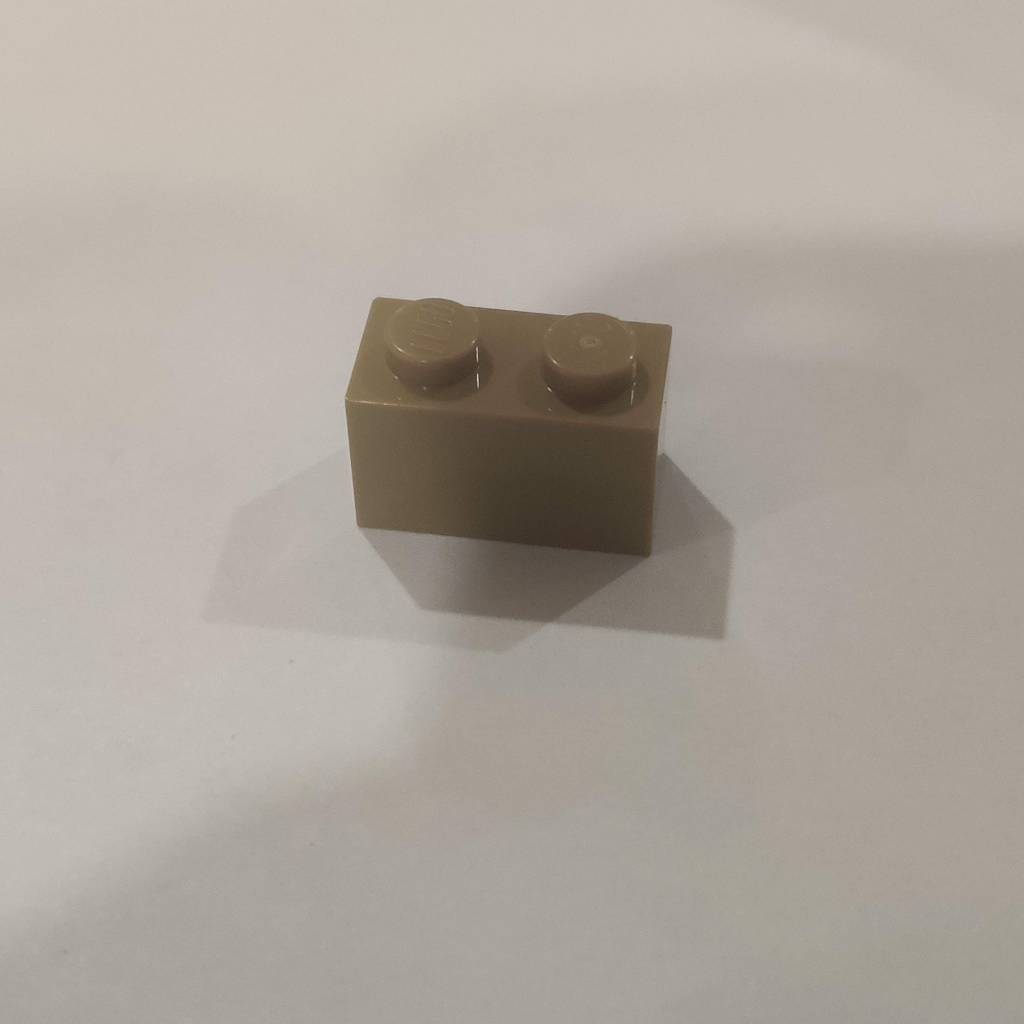
\includegraphics[width=\textwidth]{IMG_20230902_133703.jpg}
                \caption{Old Image}
            \end{subfigure}
            \begin{subfigure}[b]{0.2\textwidth}
                \centering
                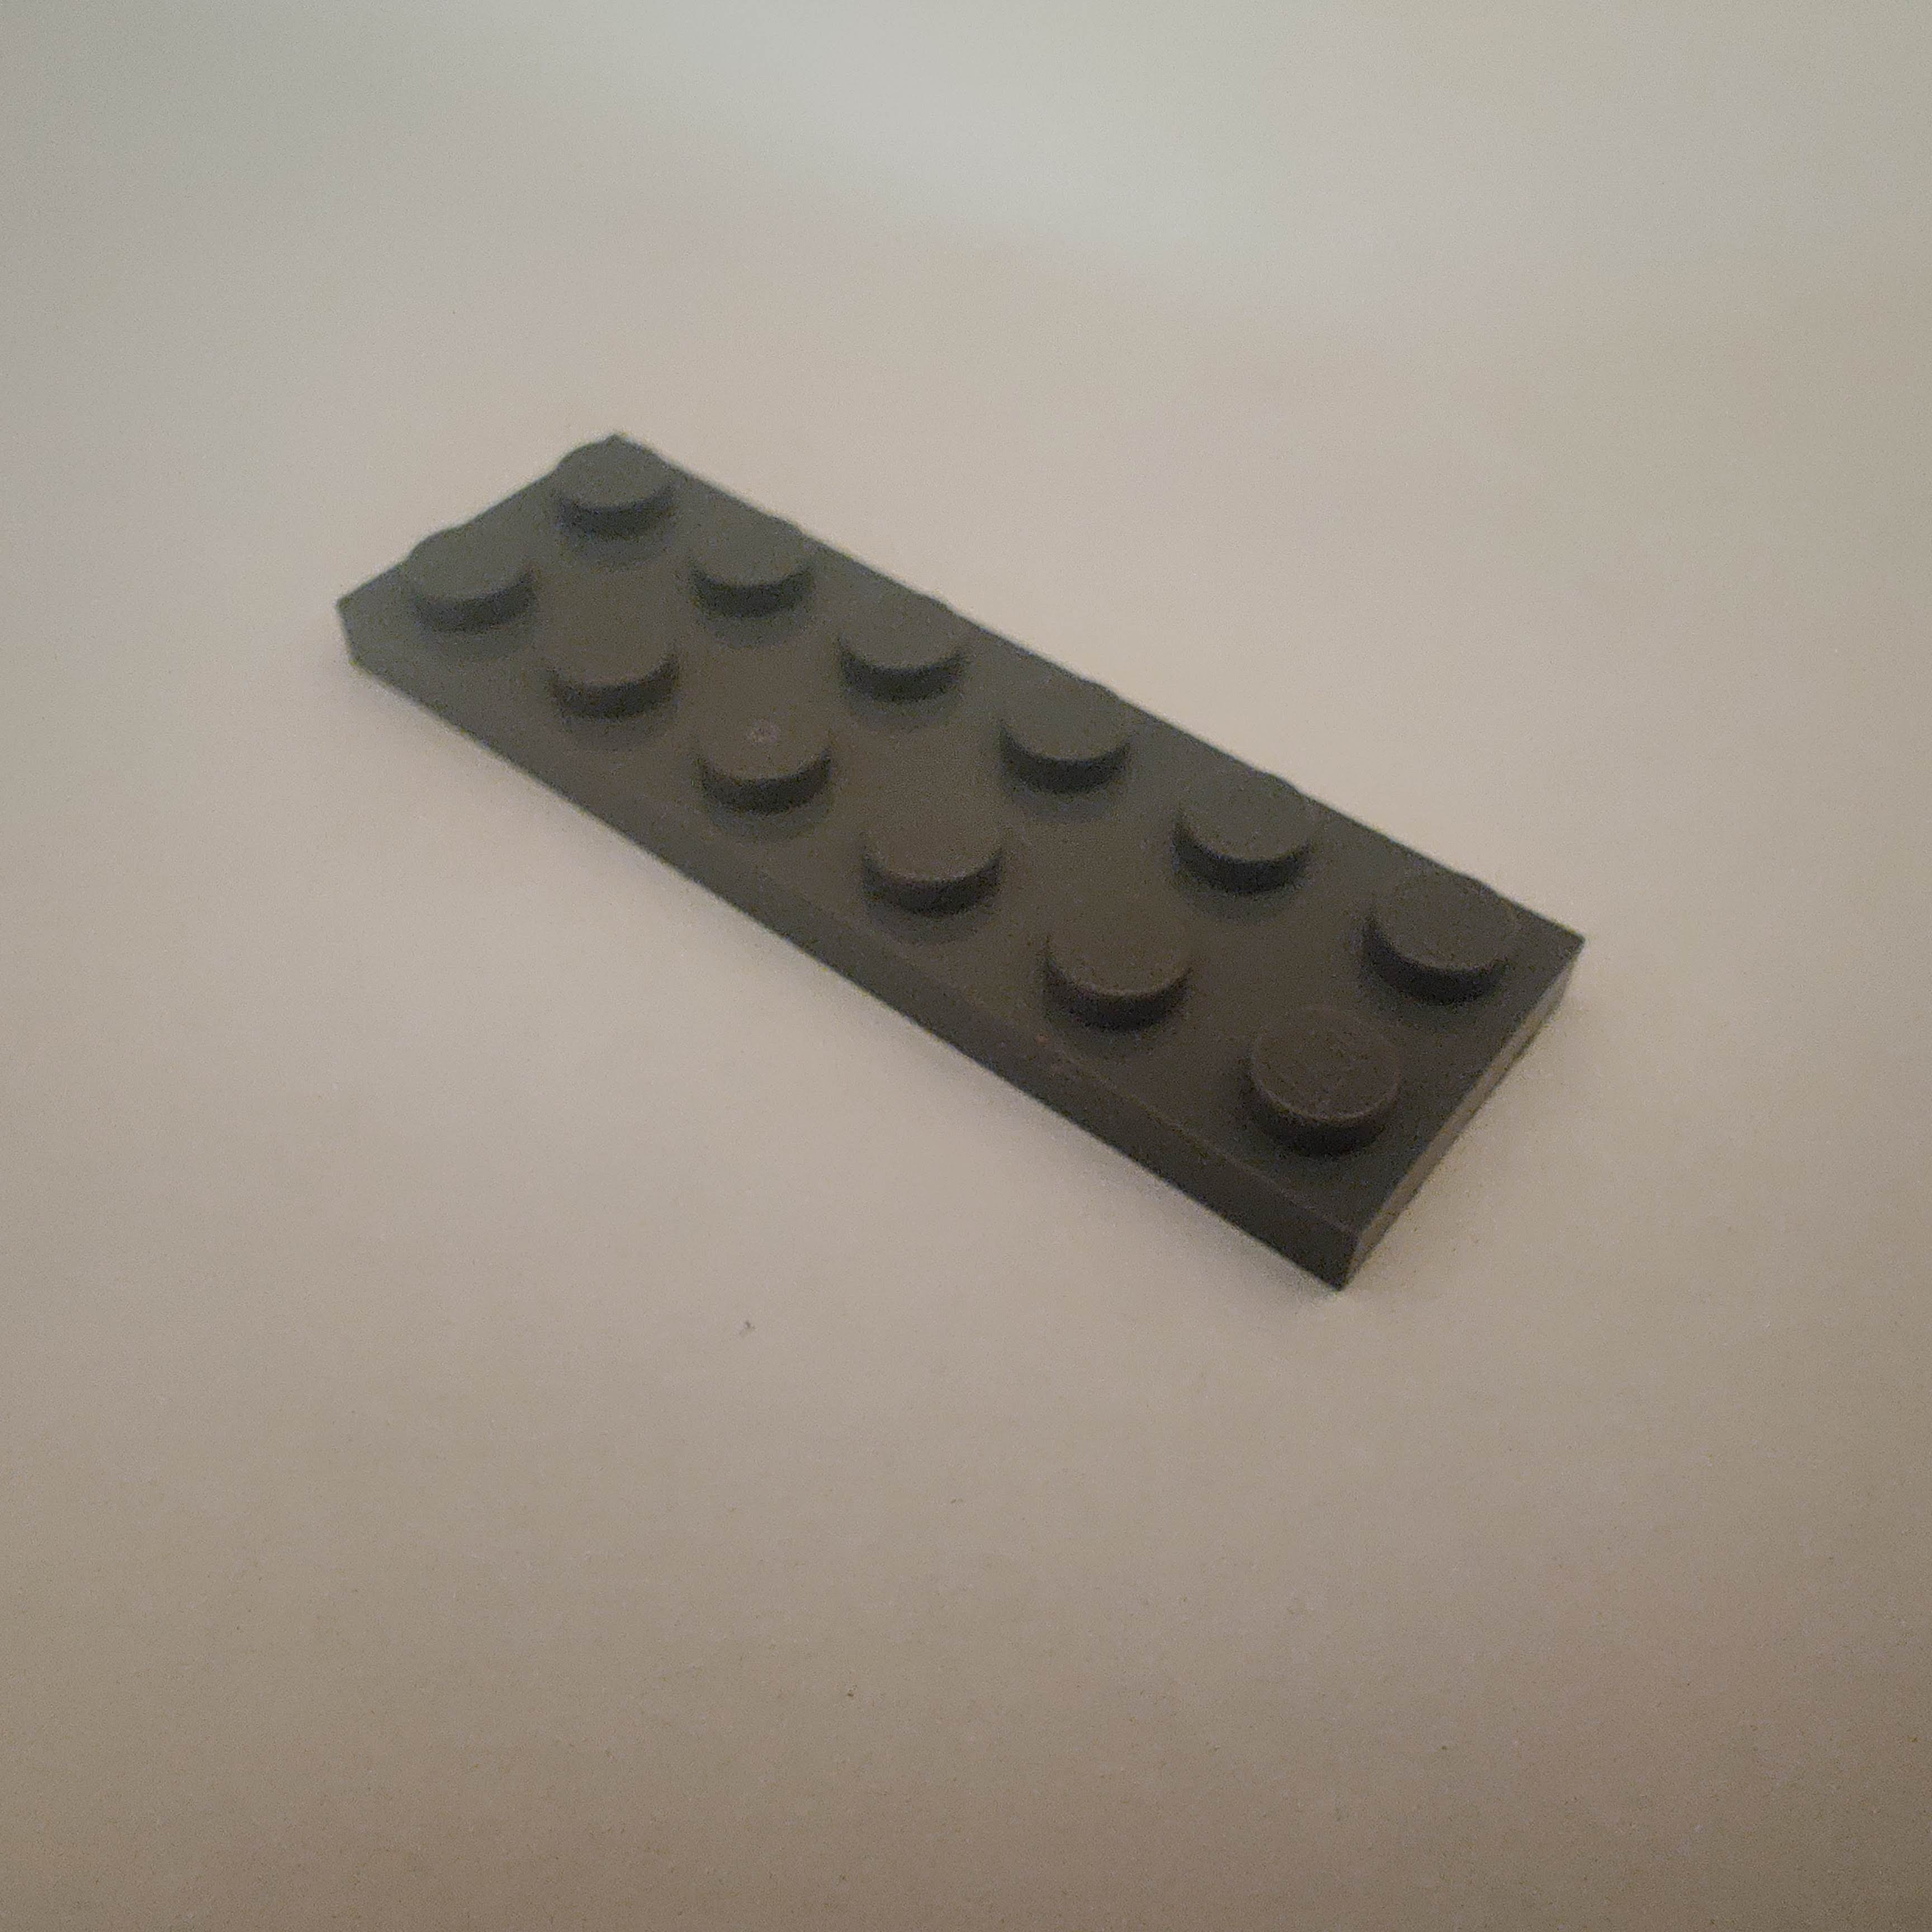
\includegraphics[width=\textwidth]{photographed images/21.jpg}
                \caption{New Image}
            \end{subfigure}\par\medskip
        \end{figure}
        \begin{itemize}
            \item Here are two examples of a previously generated image (a) and a newer image (b). We had previously generated a past dataset that has around 500 images, this dataset included (a). However, there are problems to the images: poor lighting, occluding shadows, and a pattern of a certain shadow (phone).
        \end{itemize}
        \item Computer Generated Legos:
        \begin{figure}[h]
            \centering
            \begin{subfigure}[b]{0.25\textwidth}
                \centering
                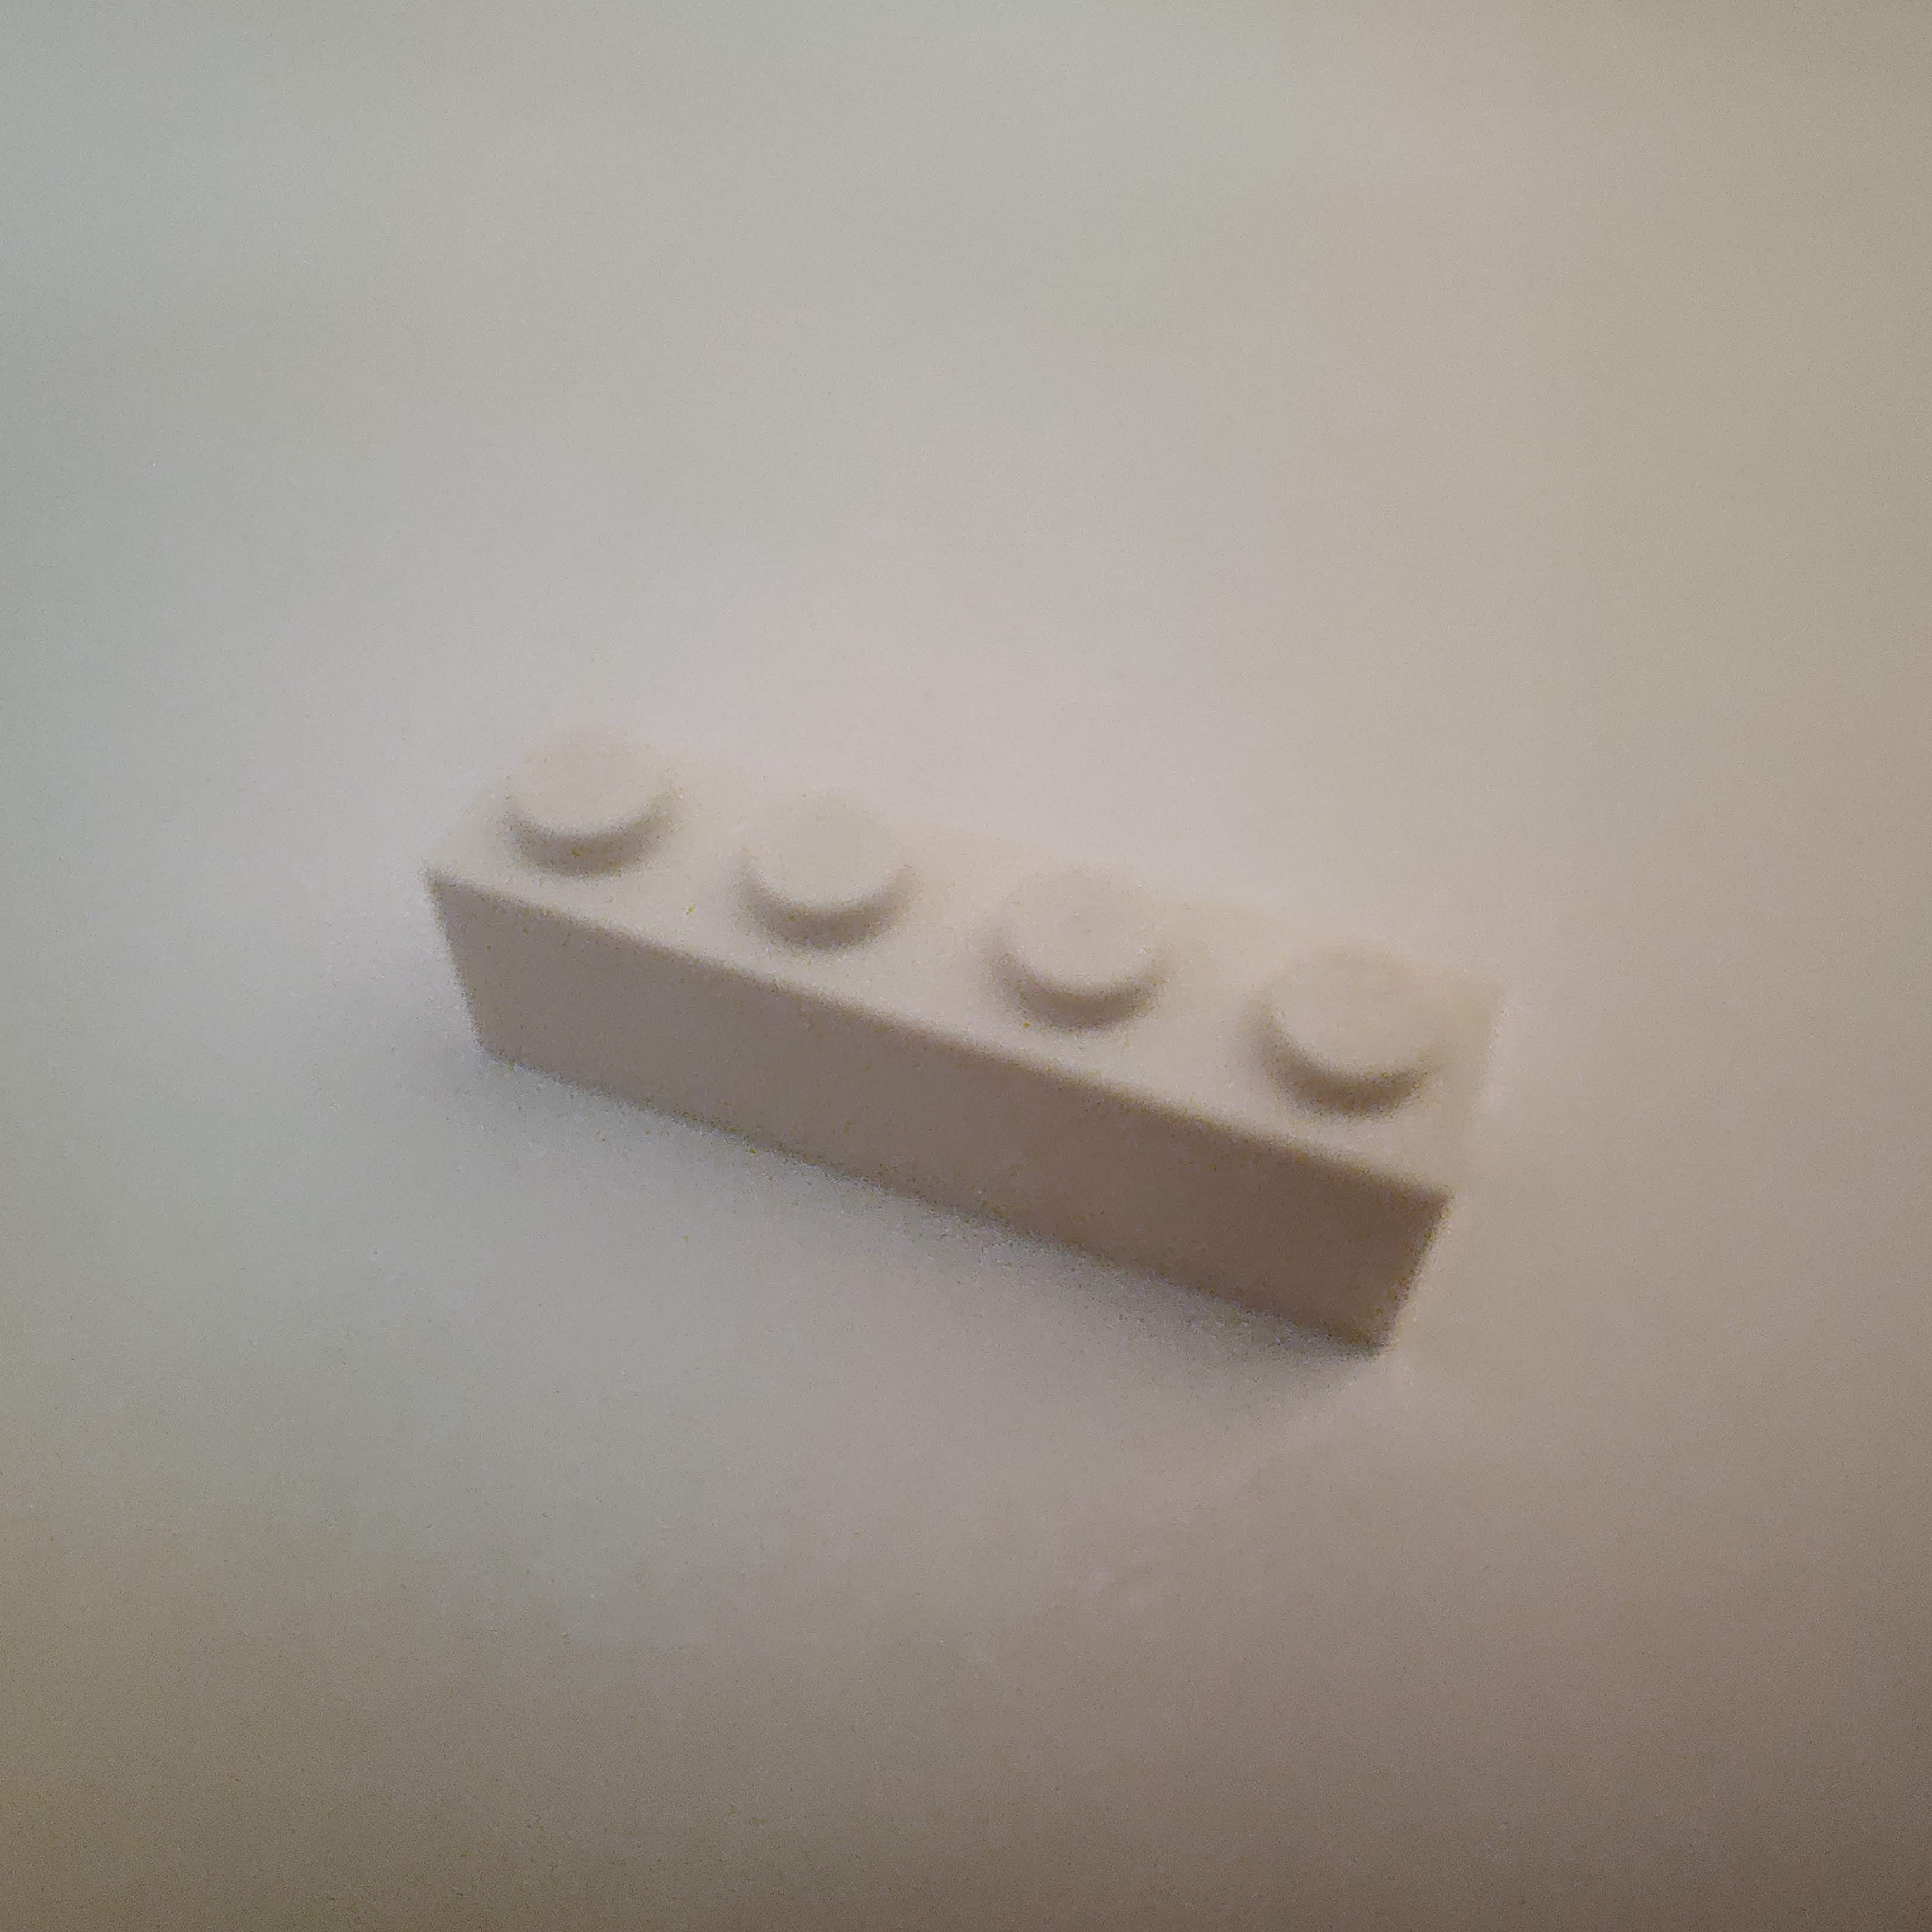
\includegraphics[width=\textwidth]{photographed images/7.jpg}
                \caption{Photographed}
            \end{subfigure}
            \begin{subfigure}[b]{0.25\textwidth}
                \centering
                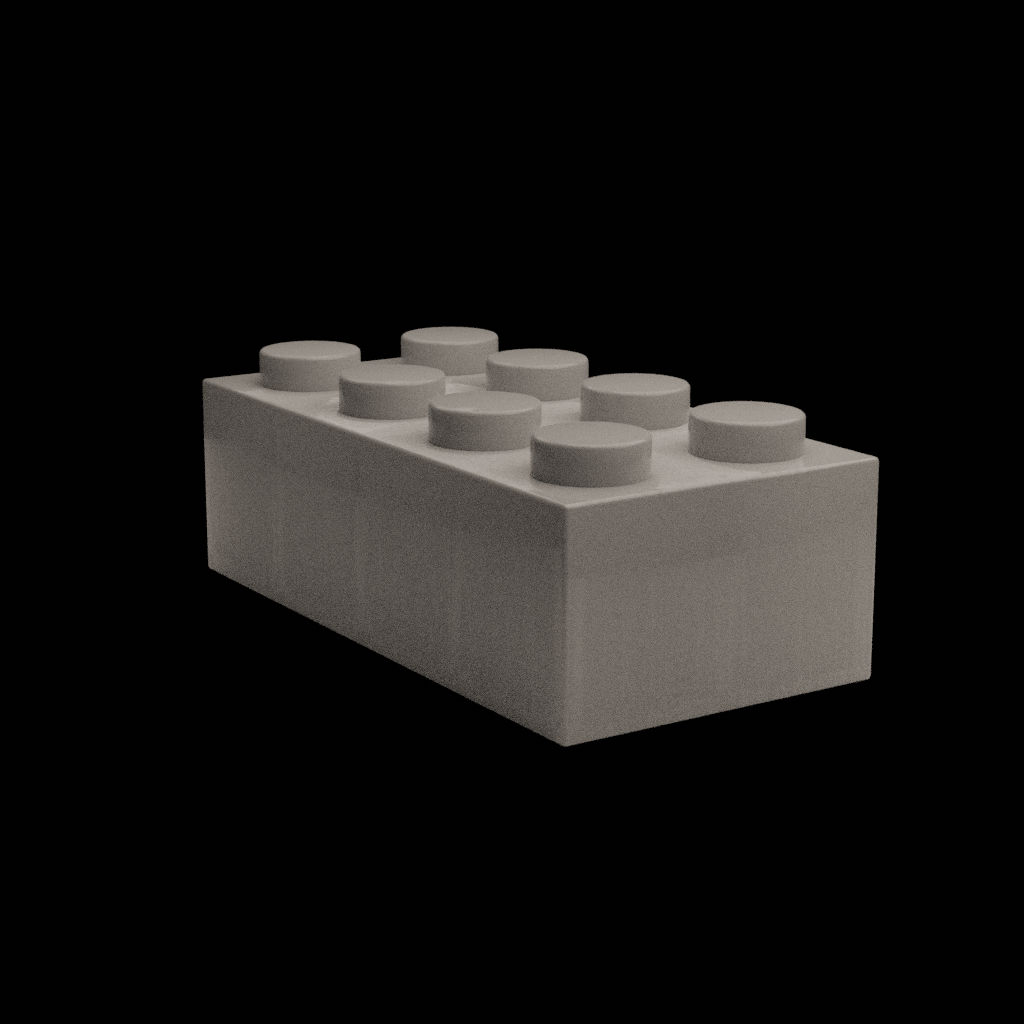
\includegraphics[width=\textwidth]{generated images/50.png}
                \caption{Computer Generated}
            \end{subfigure}\par\medskip
        \end{figure}
        \begin{itemize}
            \item Here are two examples of a photographed image (a) and a computer generated image (b). As you can see, the computer generated image is cleaner, has no background effects (shadow), and clearly represents the lego in the correct space at the correct angle at all times. We used both datasets in our VAE.
        \end{itemize}
    \end{itemize}
    \item Data Augmentation:
    \begin{itemize}
        \item Data augmentation pipeline: (image) $\Rightarrow$ (mirror) $\Rightarrow$ (greyscale)
        \item In our original two datasets, we did not augment them in the physical file. When the images are placed into a dataset on python, we augmented the images by mirroring them. This allowed us to double our dataset size and still maintain a bit of a uniqueness.
        \item We did not choose to rotate or flip due to the fact that a flipped lego piece or rotated lego piece will confuse the model based on dimensional and perspective. That means, when the VAE attempts to learn the shape and perspective of the general lego piece, it will have a harder time trying to understand in which axis it should be in the right position. For example, if we have a lego rotated 30 degrees, should it be compared to that way or should it be compared to as if it were on the ground?
    \end{itemize}
\end{enumerate}

\begin{figure}[h]
    \centering
    \begin{subfigure}[b]{0.2\textwidth}
        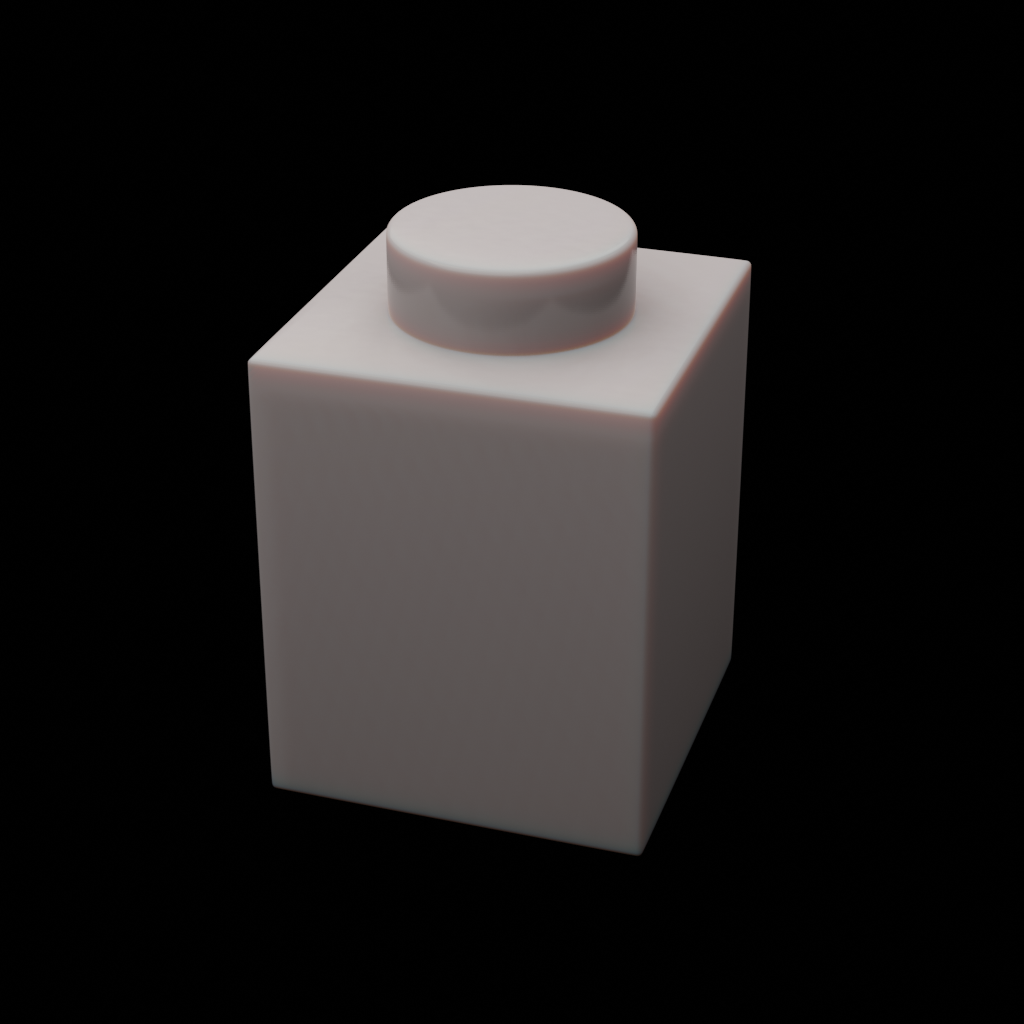
\includegraphics[width=\textwidth]{generated images/25.png}
    \end{subfigure}
    \begin{subfigure}[b]{0.2\textwidth}
        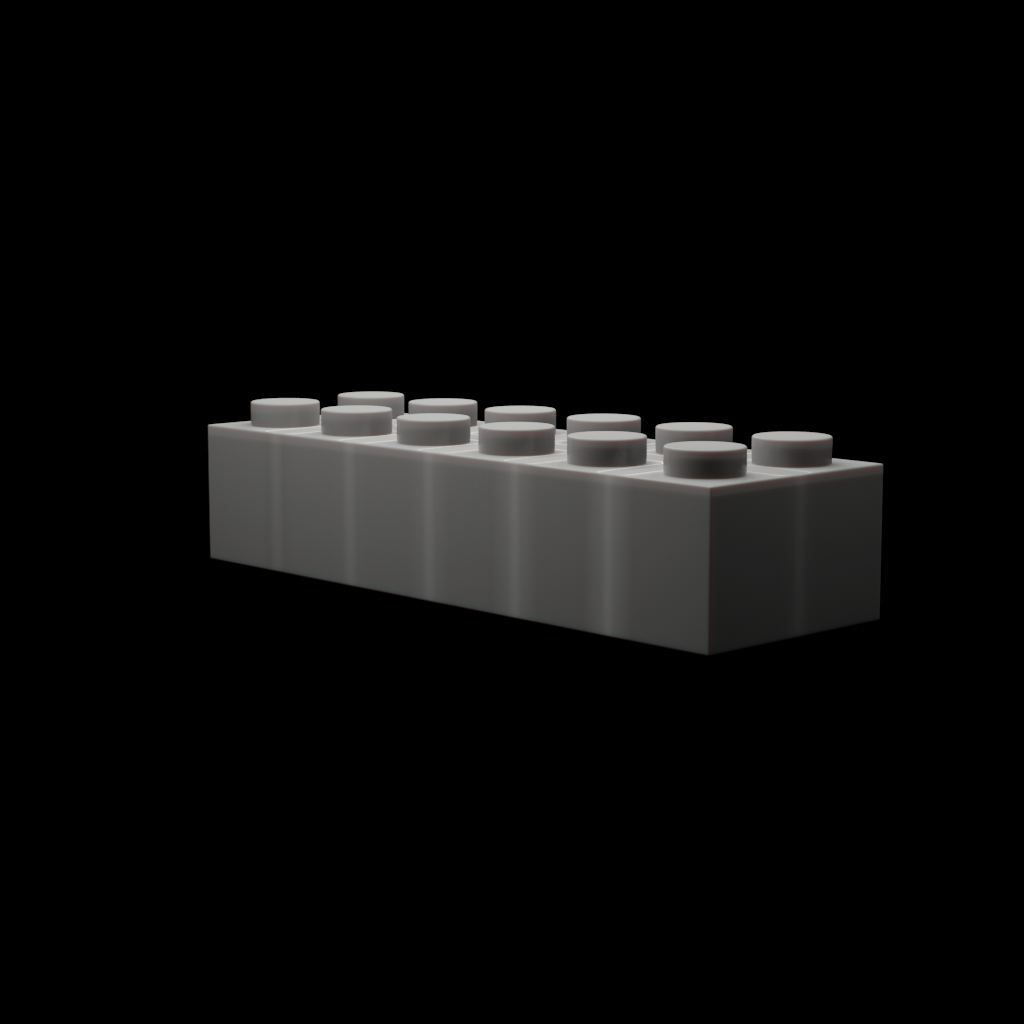
\includegraphics[width=\textwidth]{generated images/26.png}
    \end{subfigure}
    \begin{subfigure}[b]{0.2\textwidth}
        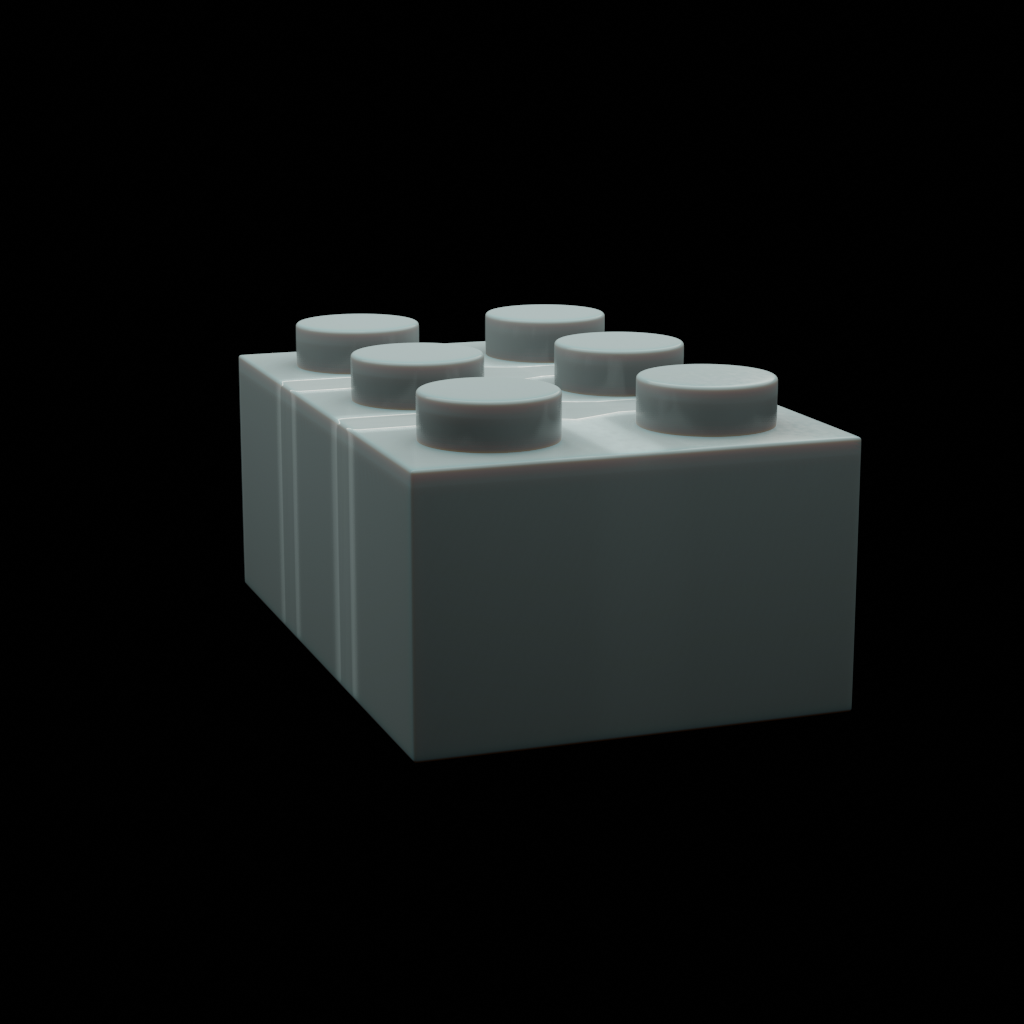
\includegraphics[width=\textwidth]{generated images/27.png}
    \end{subfigure}
    \begin{subfigure}[b]{0.2\textwidth}
        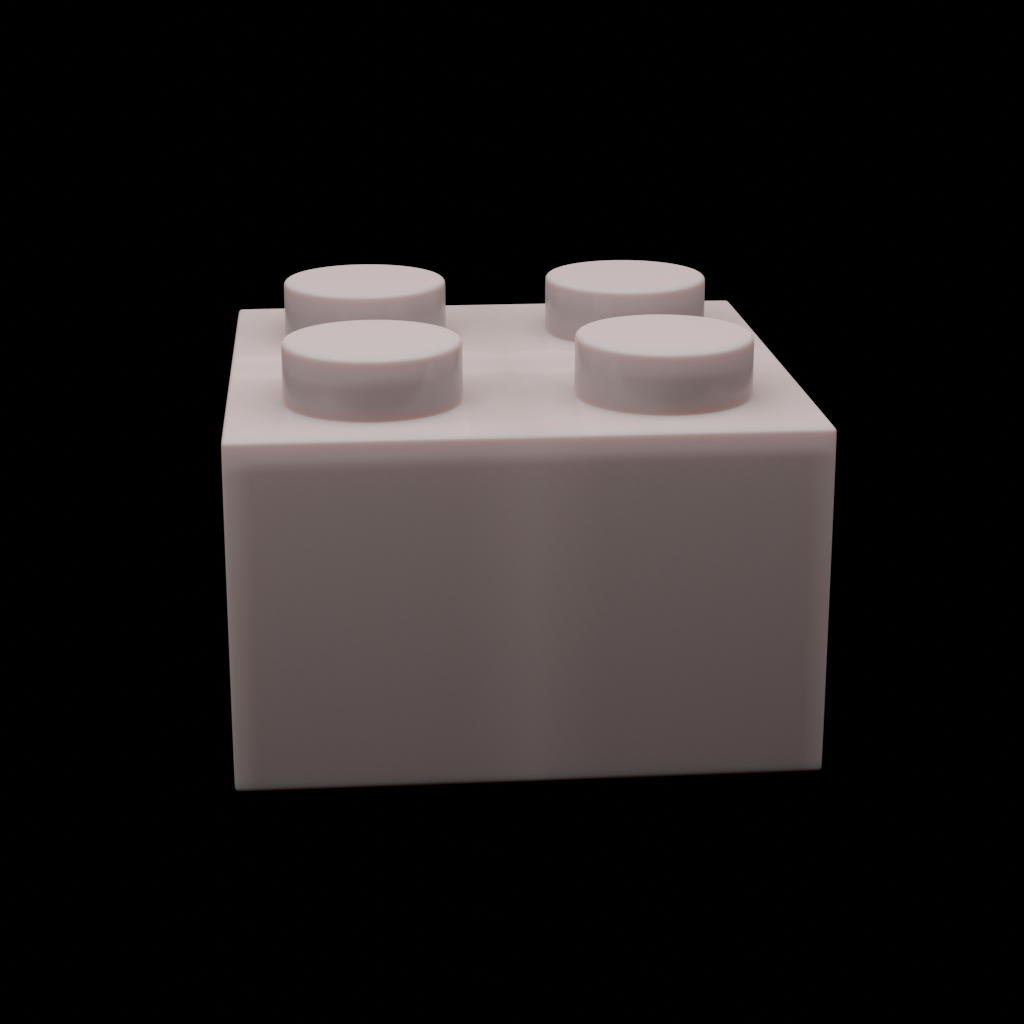
\includegraphics[width=\textwidth]{generated images/28.png}
    \end{subfigure}
    \begin{subfigure}[b]{0.2\textwidth}
        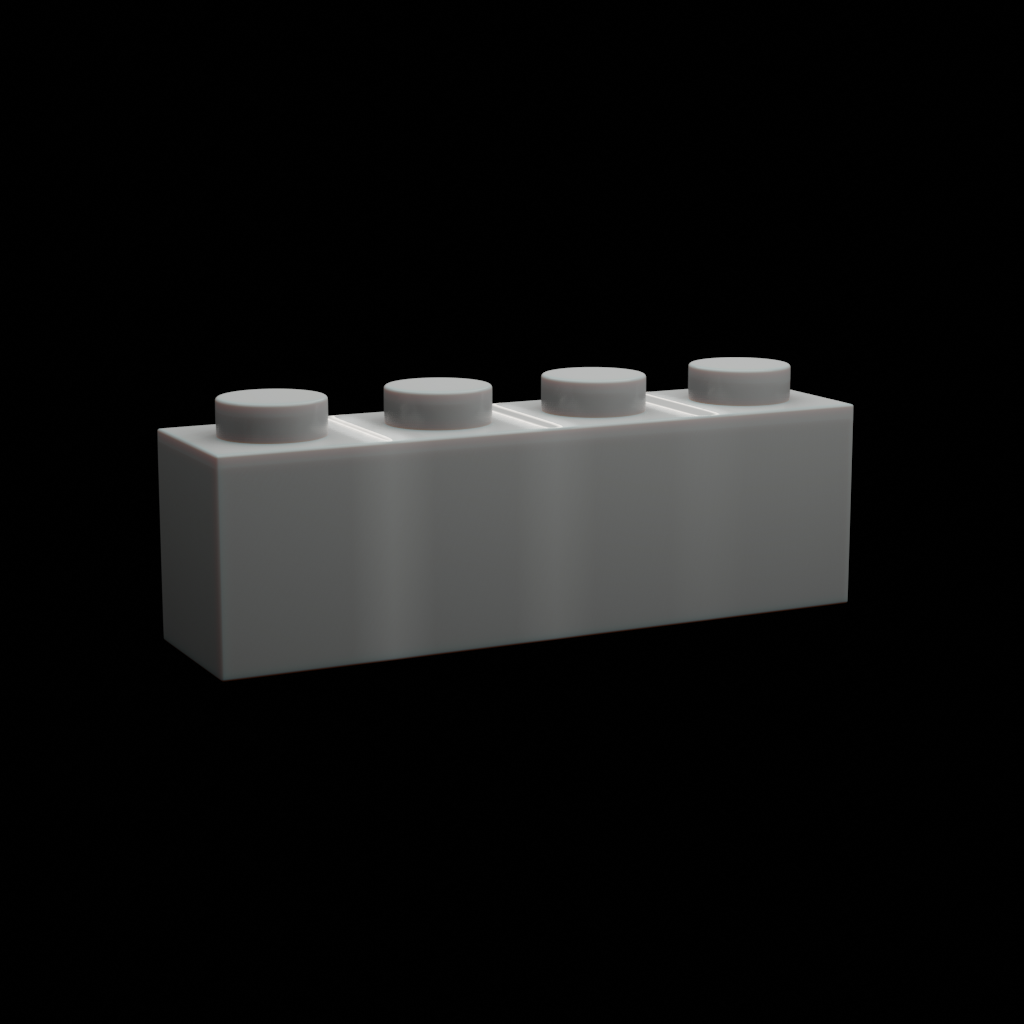
\includegraphics[width=\textwidth]{generated images/29.png}
    \end{subfigure}
    \begin{subfigure}[b]{0.2\textwidth}
        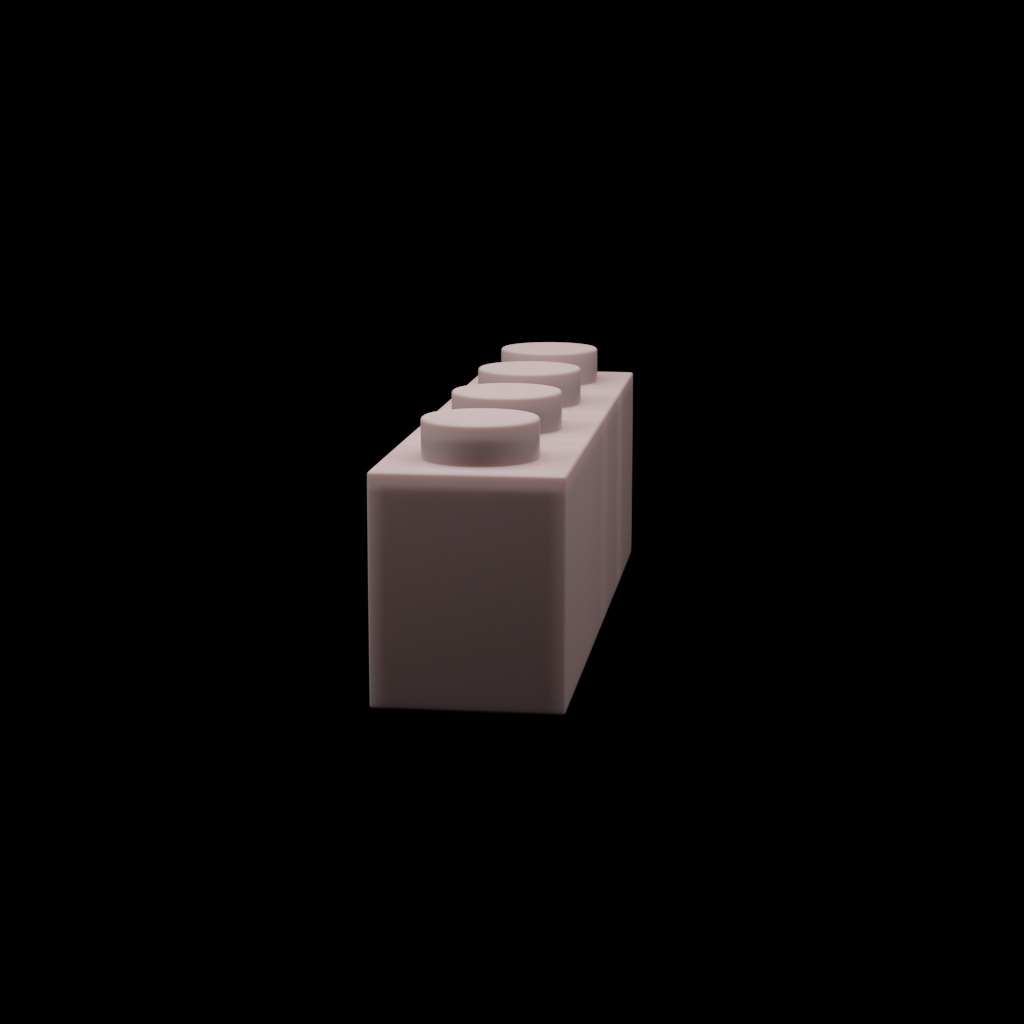
\includegraphics[width=\textwidth]{generated images/30.png}
    \end{subfigure}
    \begin{subfigure}[b]{0.2\textwidth}
        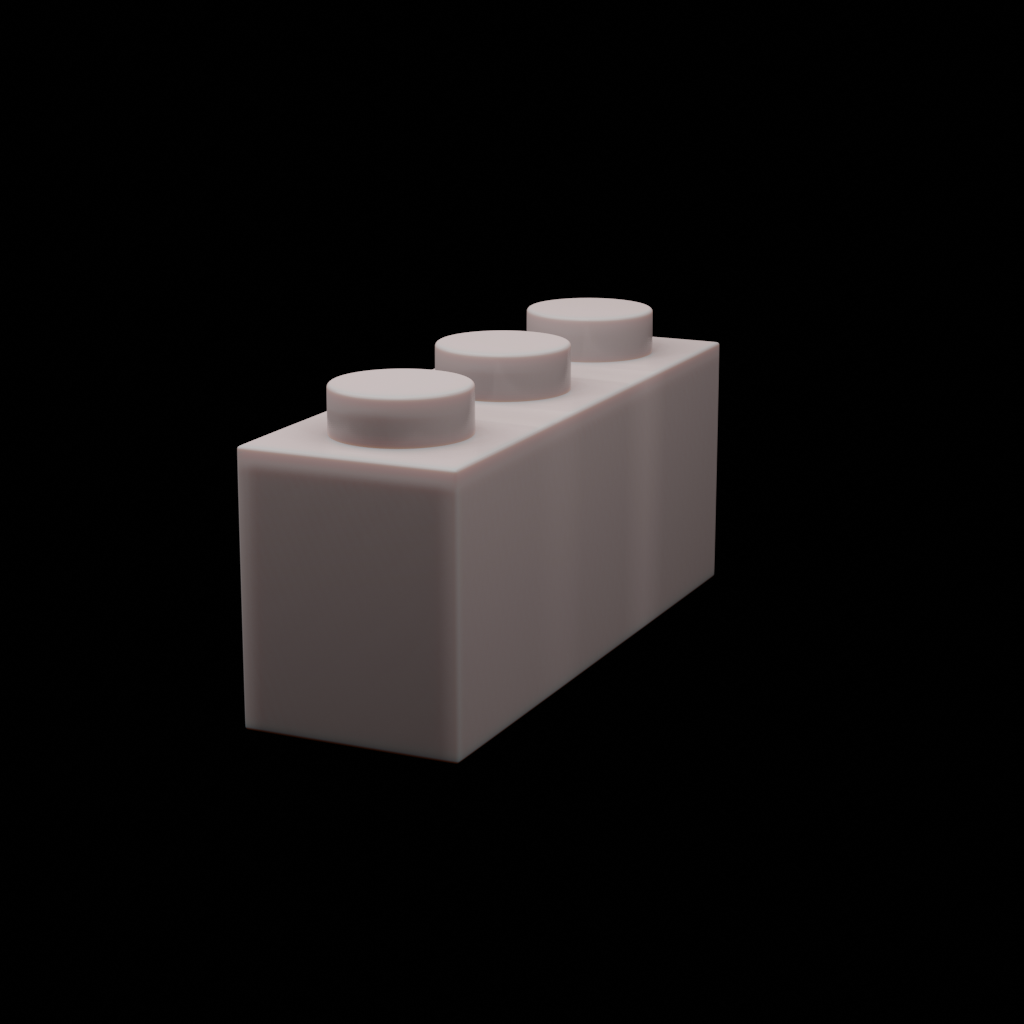
\includegraphics[width=\textwidth]{generated images/31.png}
    \end{subfigure}
    \begin{subfigure}[b]{0.2\textwidth}
        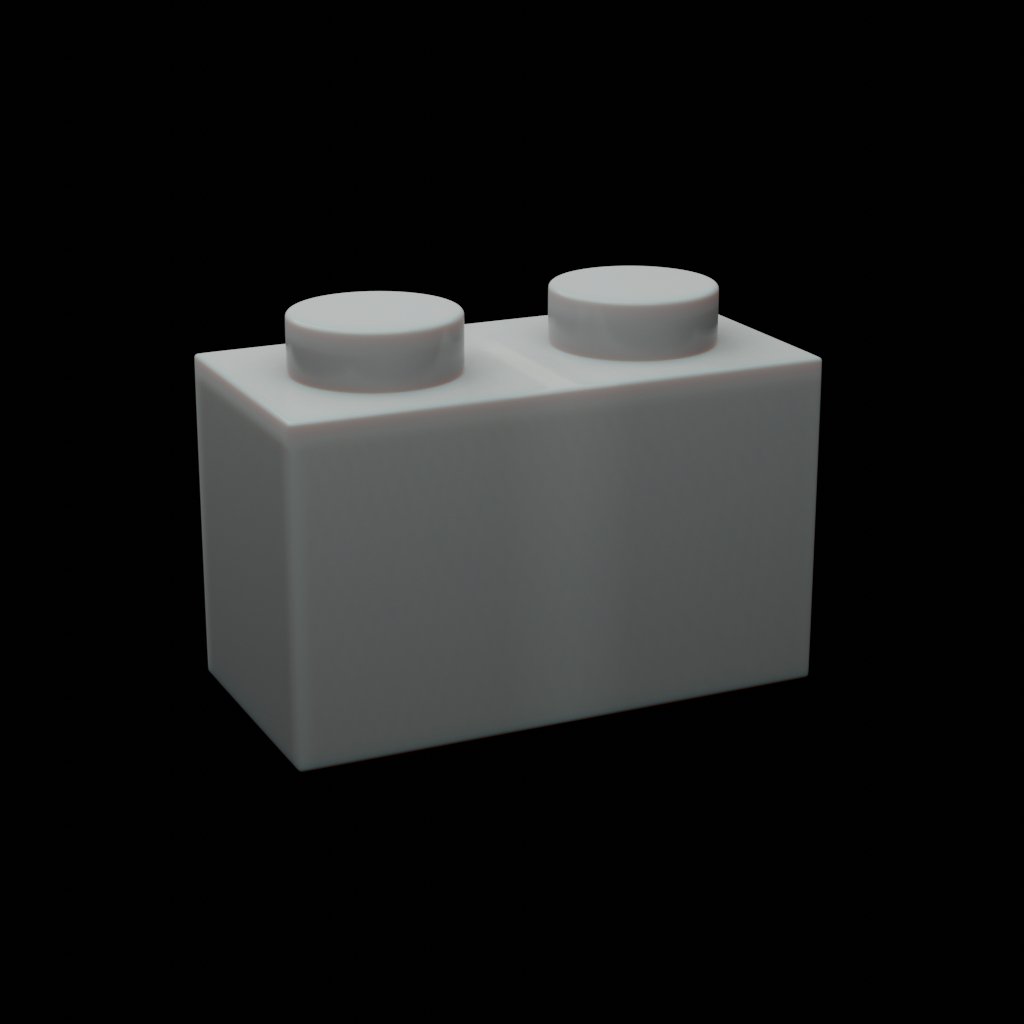
\includegraphics[width=\textwidth]{generated images/32.png}
    \end{subfigure}
    \begin{subfigure}[b]{0.2\textwidth}
        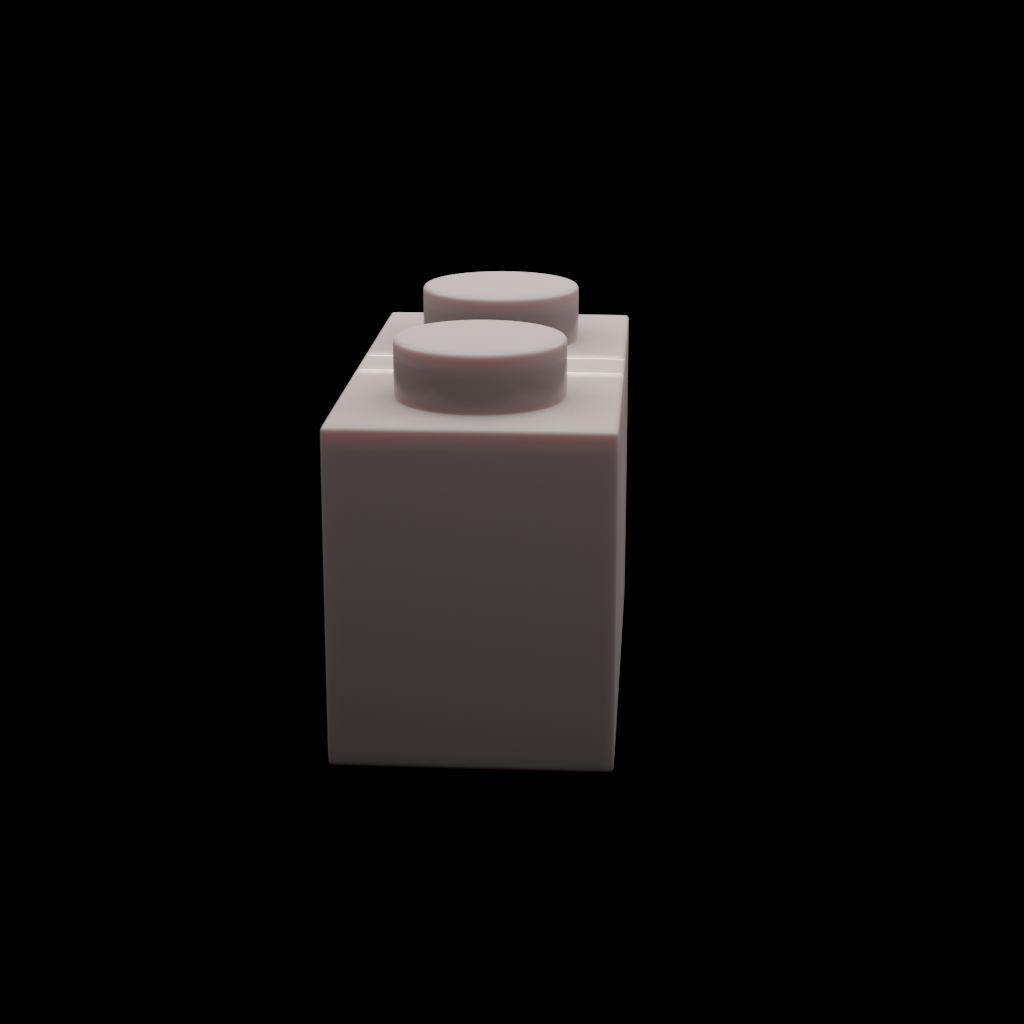
\includegraphics[width=\textwidth]{generated images/33.png}
    \end{subfigure}
    \begin{subfigure}[b]{0.2\textwidth}
        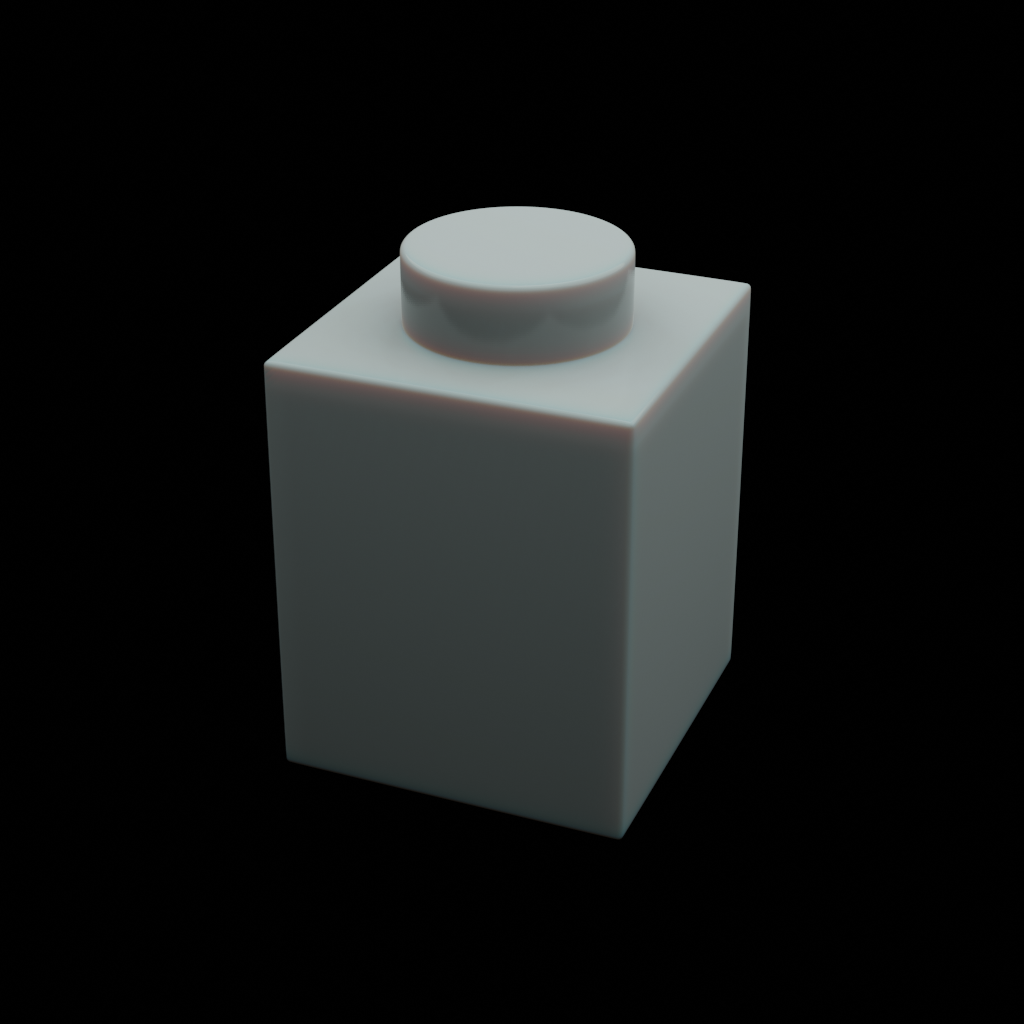
\includegraphics[width=\textwidth]{generated images/34.png}
    \end{subfigure}
    \begin{subfigure}[b]{0.2\textwidth}
        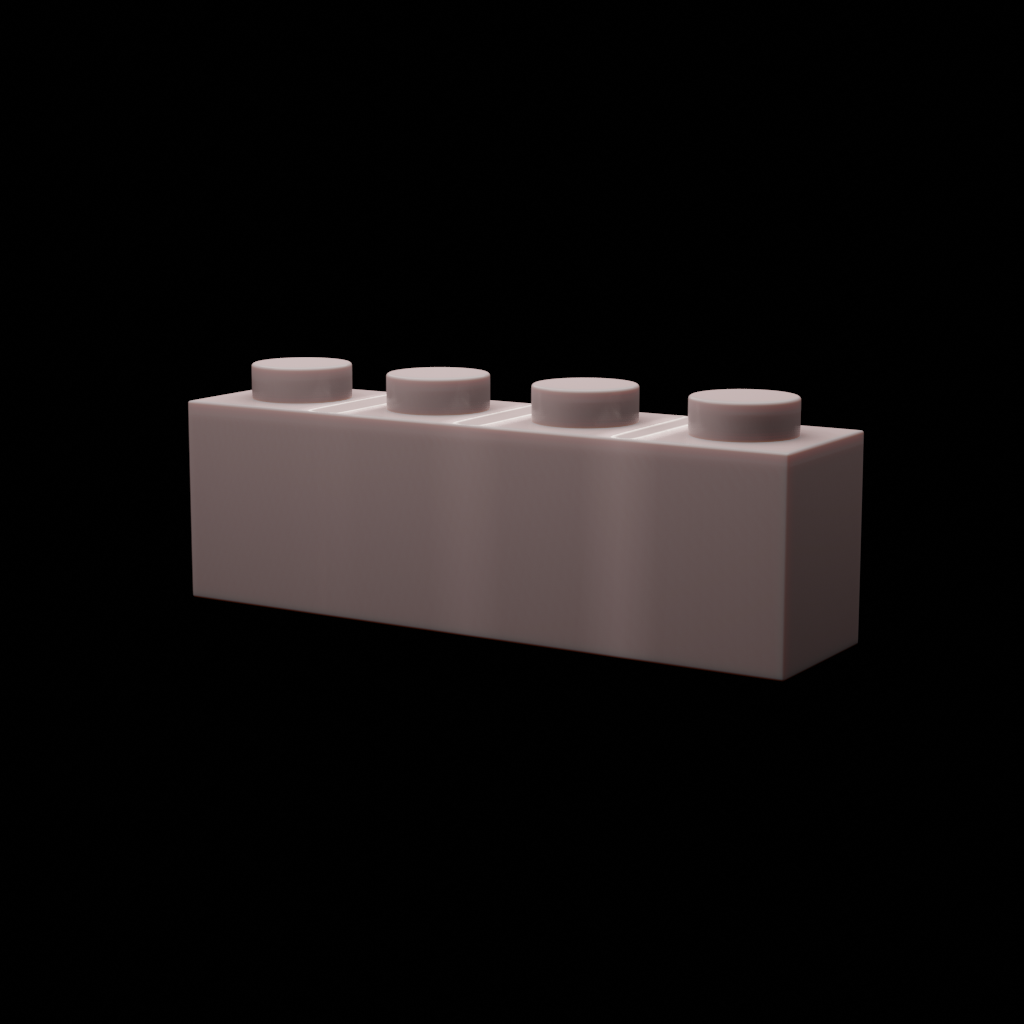
\includegraphics[width=\textwidth]{generated images/35.png}
    \end{subfigure}
    \begin{subfigure}[b]{0.2\textwidth}
        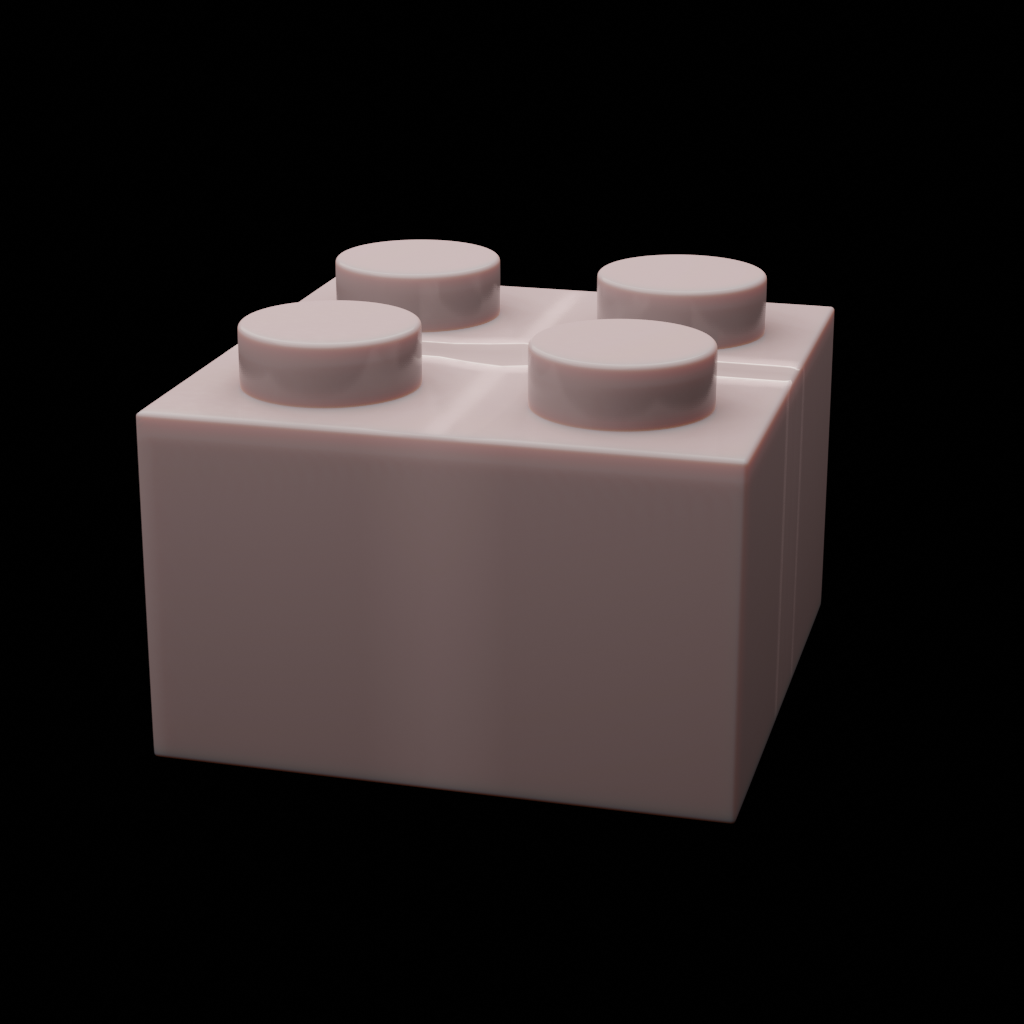
\includegraphics[width=\textwidth]{generated images/36.png}
    \end{subfigure}
    \begin{subfigure}[b]{0.2\textwidth}
        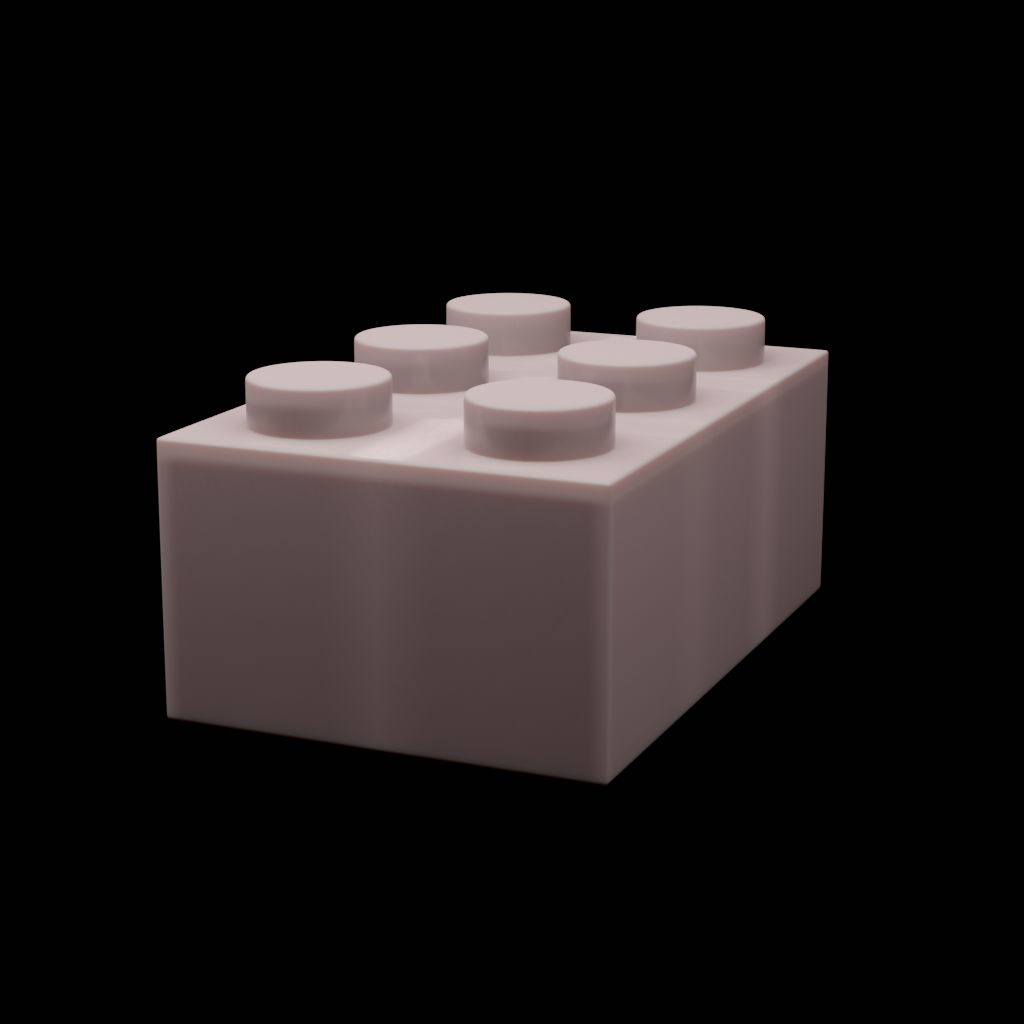
\includegraphics[width=\textwidth]{generated images/37.png}
    \end{subfigure}
    \begin{subfigure}[b]{0.2\textwidth}
        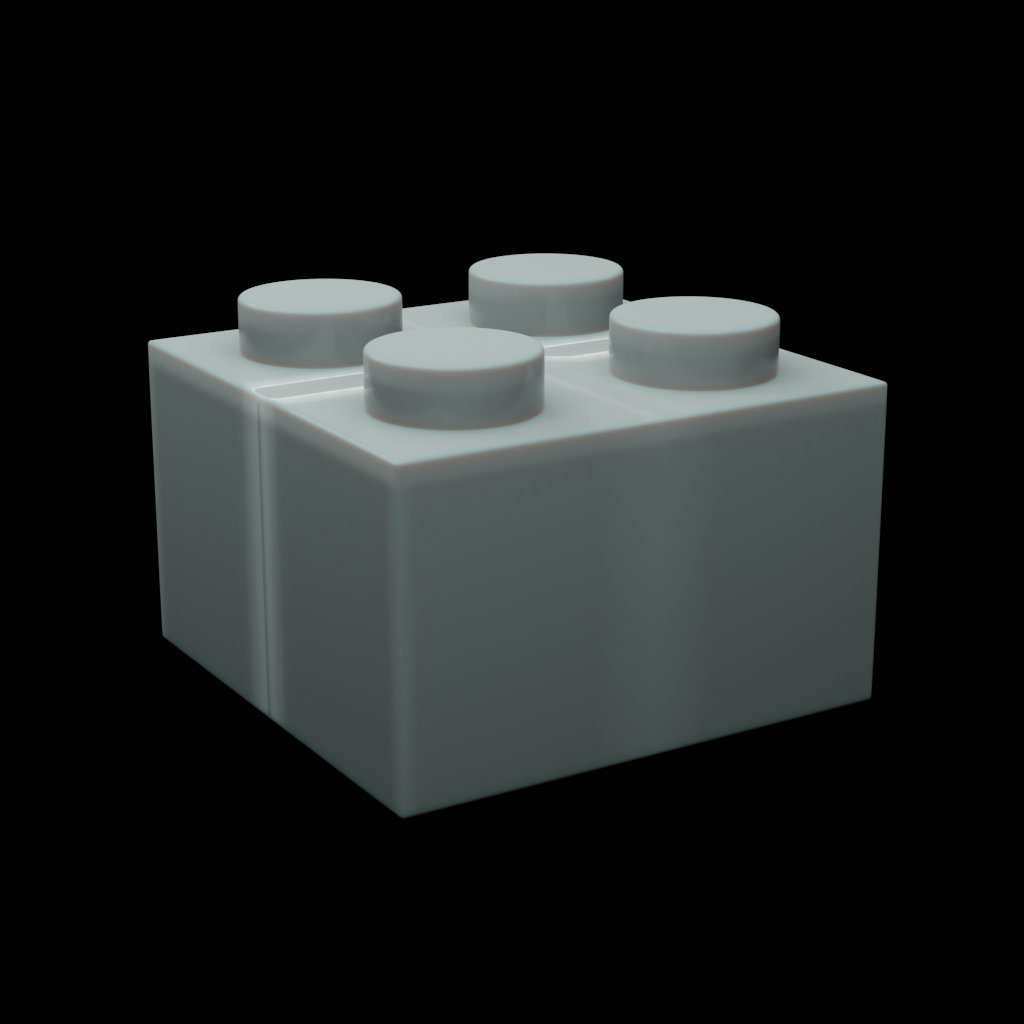
\includegraphics[width=\textwidth]{generated images/38.png}
    \end{subfigure}
    \begin{subfigure}[b]{0.2\textwidth}
        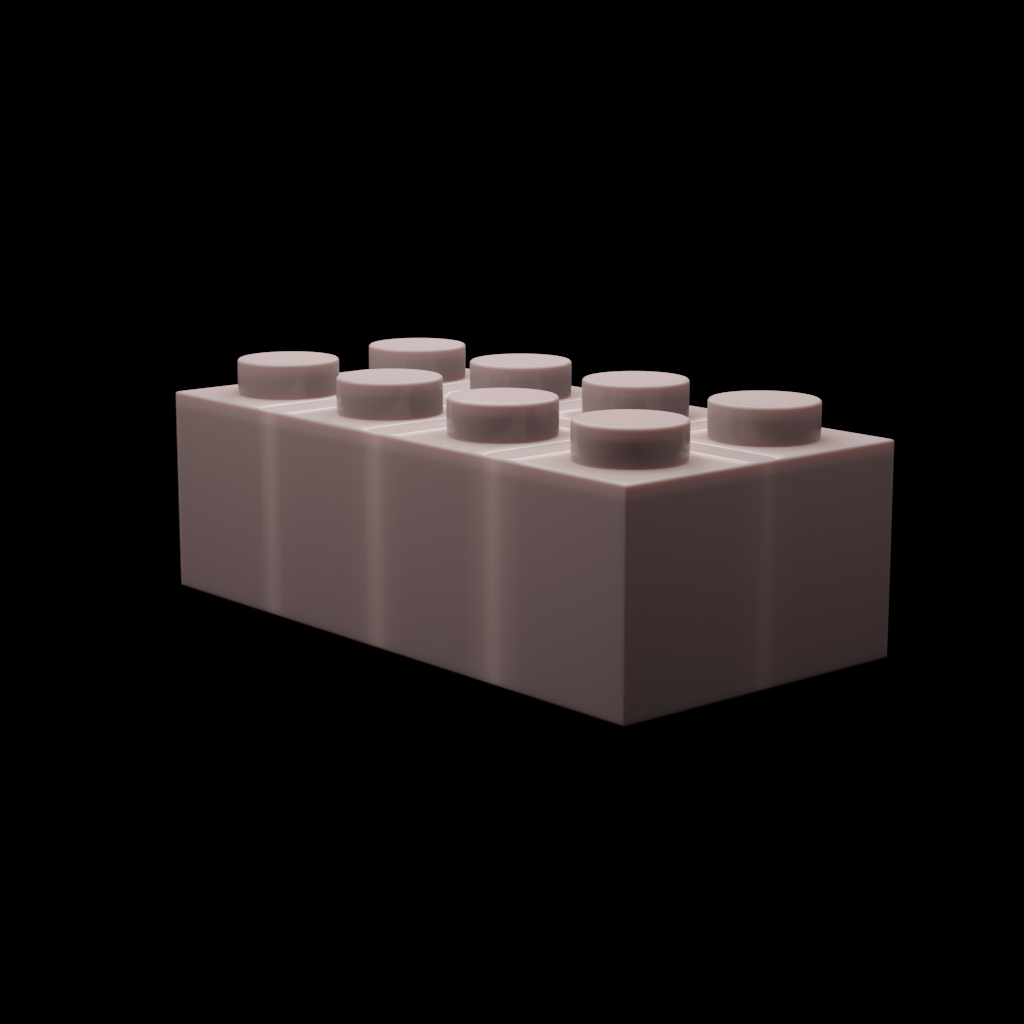
\includegraphics[width=\textwidth]{generated images/39.png}
    \end{subfigure}
    \begin{subfigure}[b]{0.2\textwidth}
        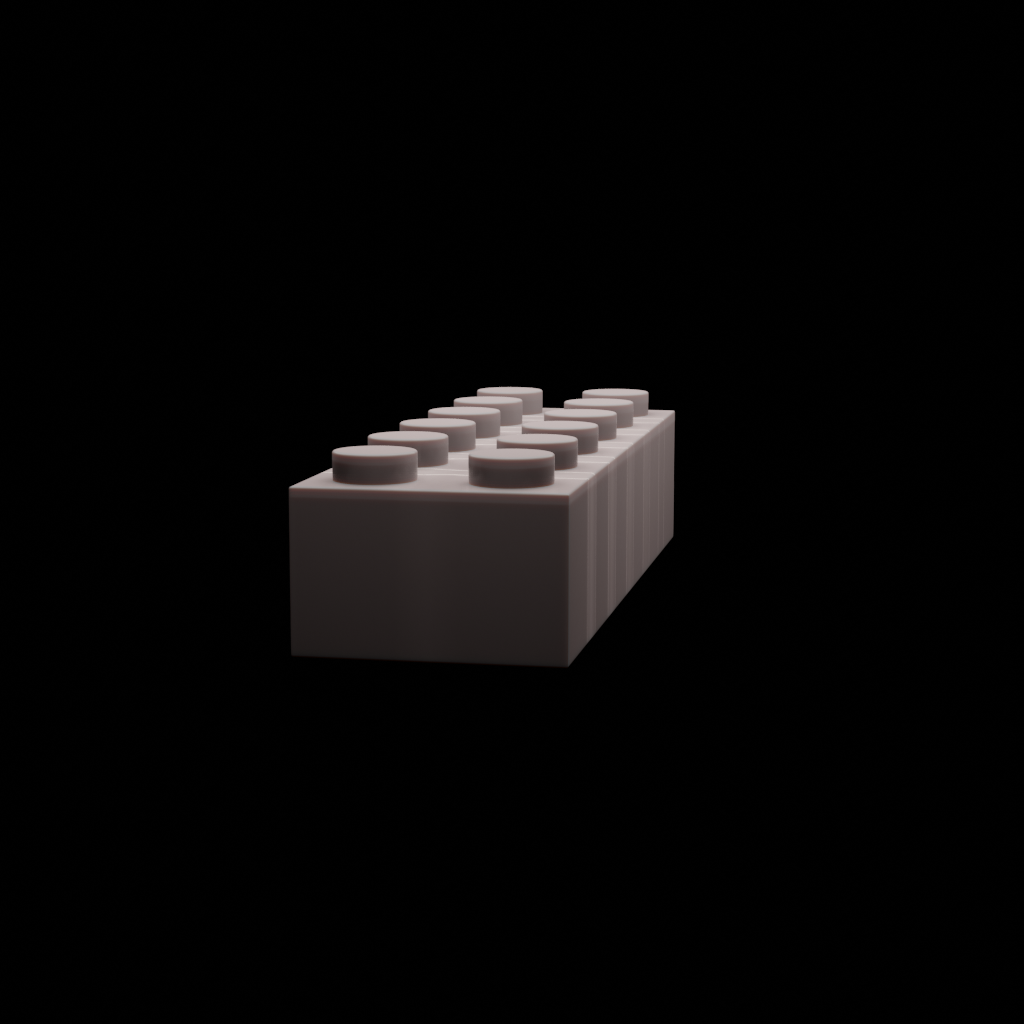
\includegraphics[width=\textwidth]{generated images/40.png}
    \end{subfigure}
    \caption{Example of the computer generated dataset}
\end{figure}

\begin{figure}[h]
    \centering
    \begin{subfigure}[b]{0.2\textwidth}
        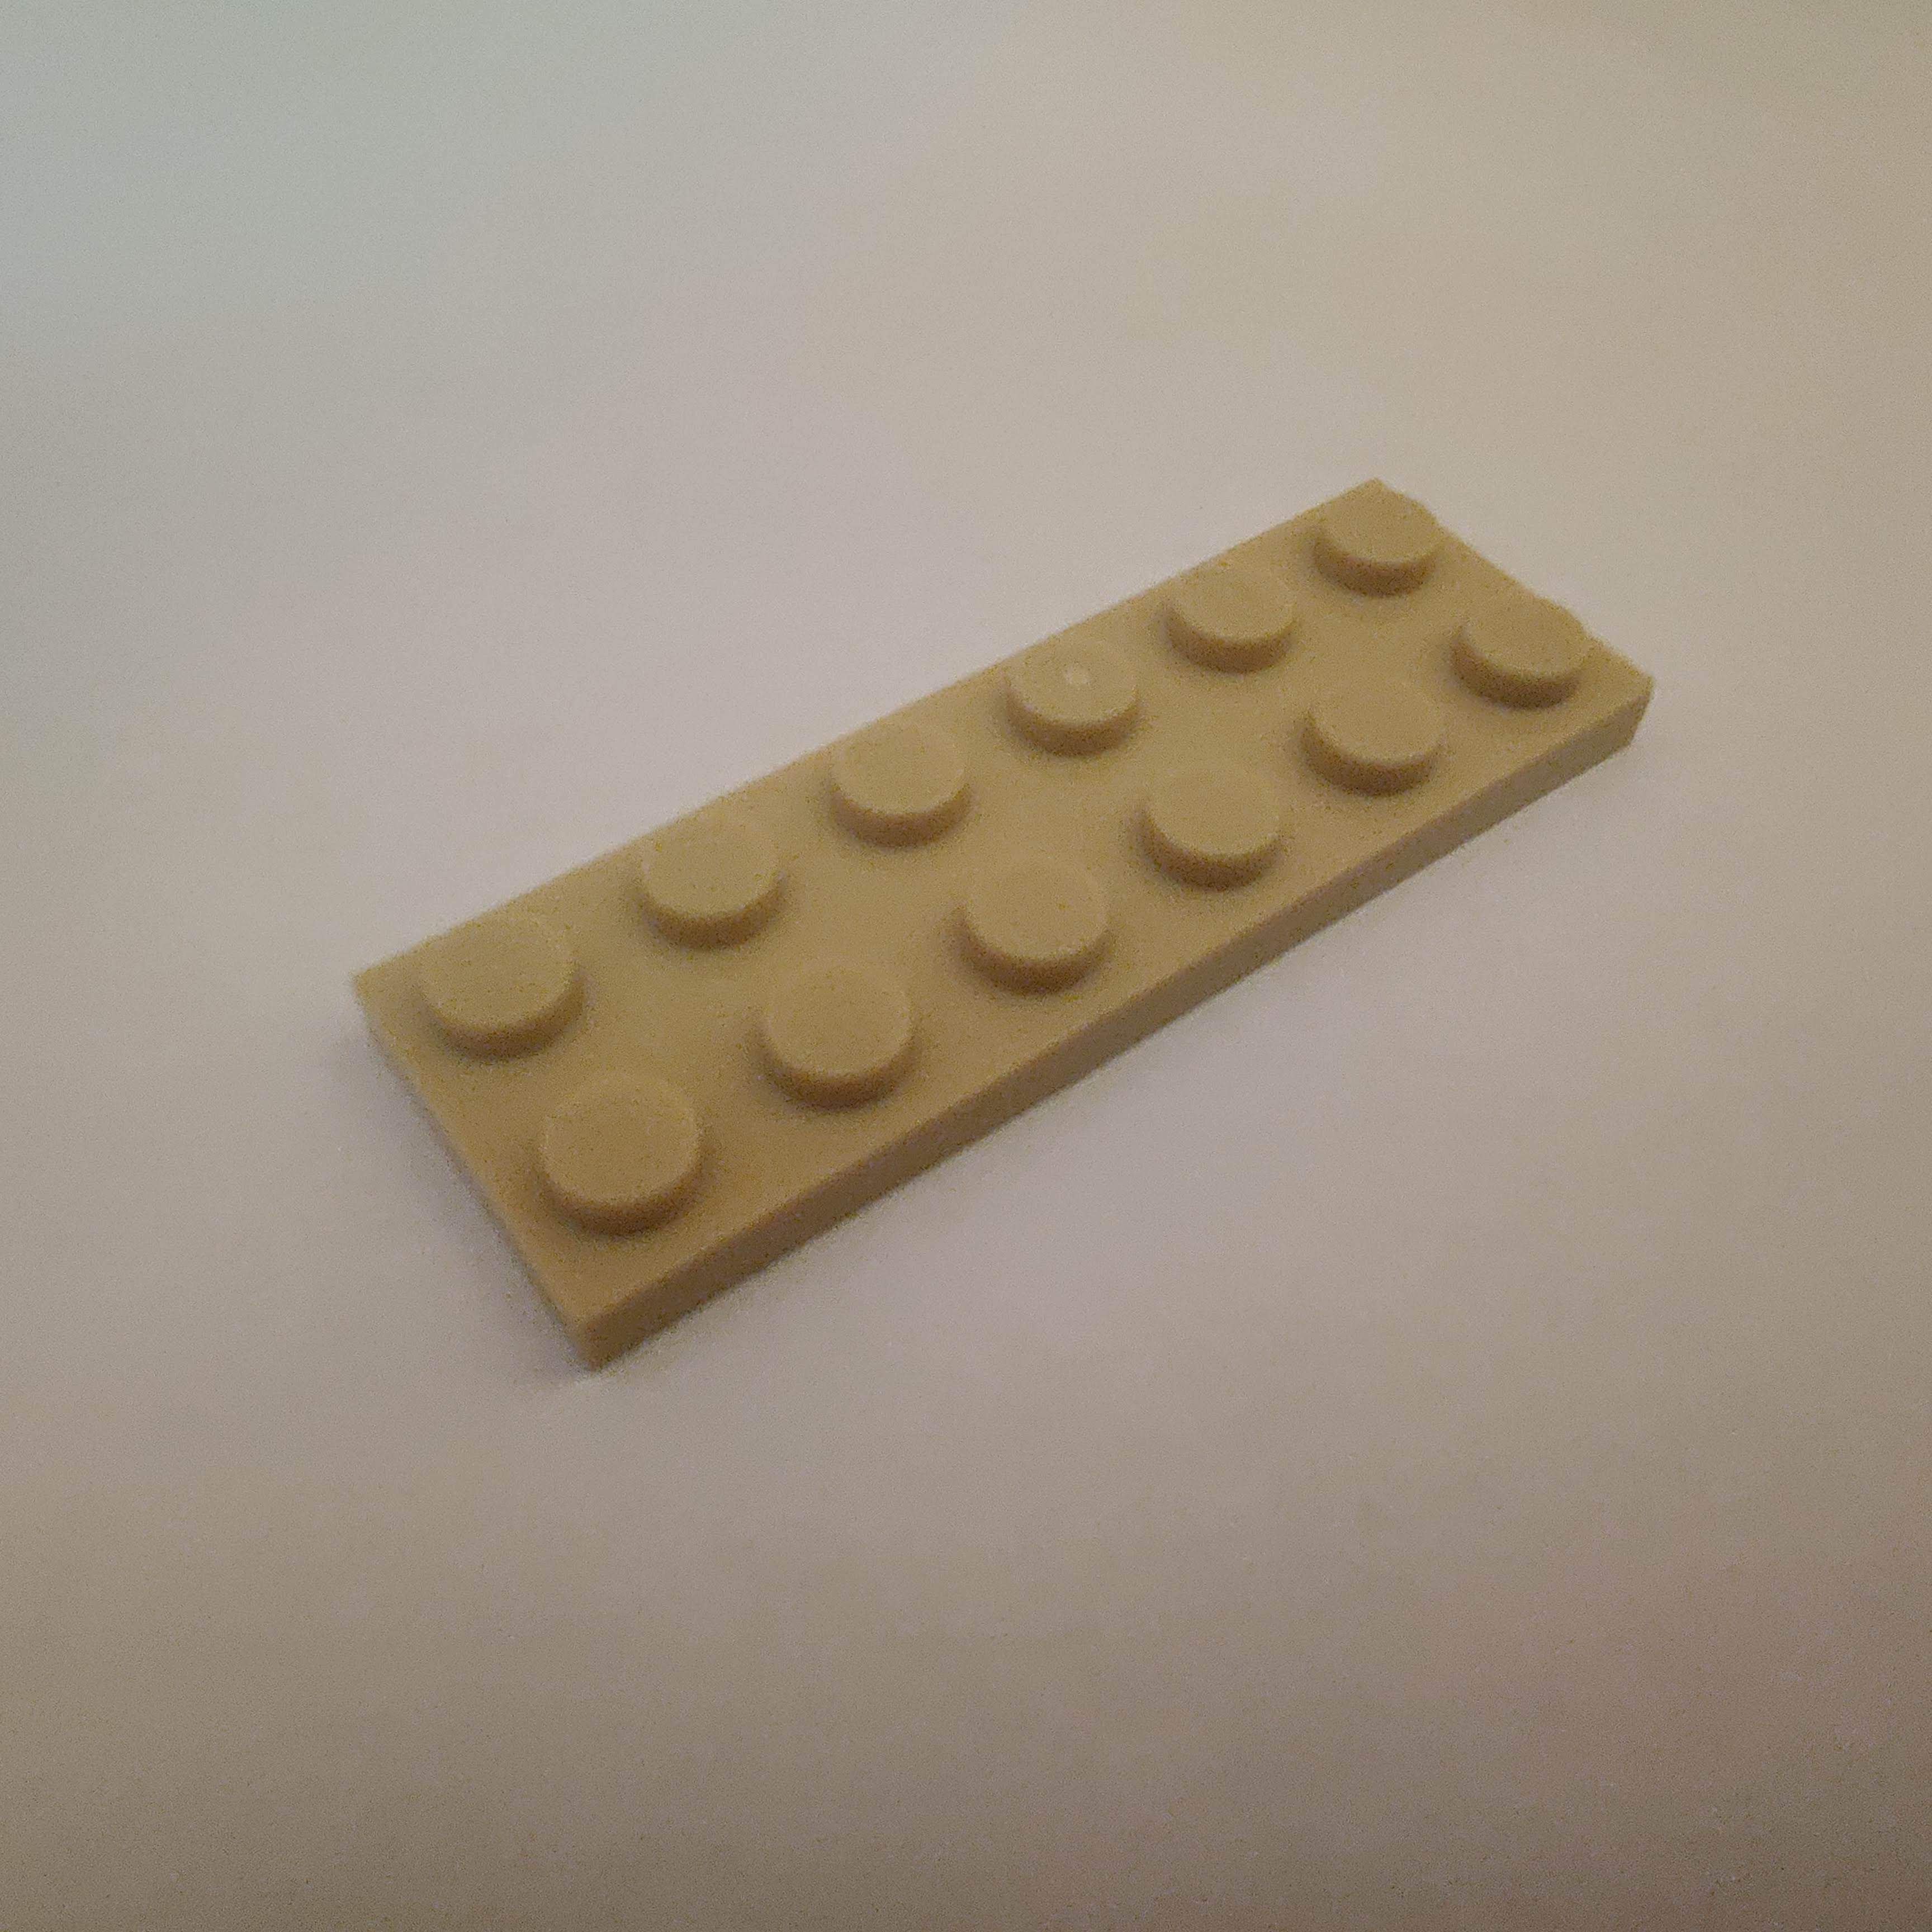
\includegraphics[width=\textwidth]{photographed images/1.jpg}
    \end{subfigure}
    \begin{subfigure}[b]{0.2\textwidth}
        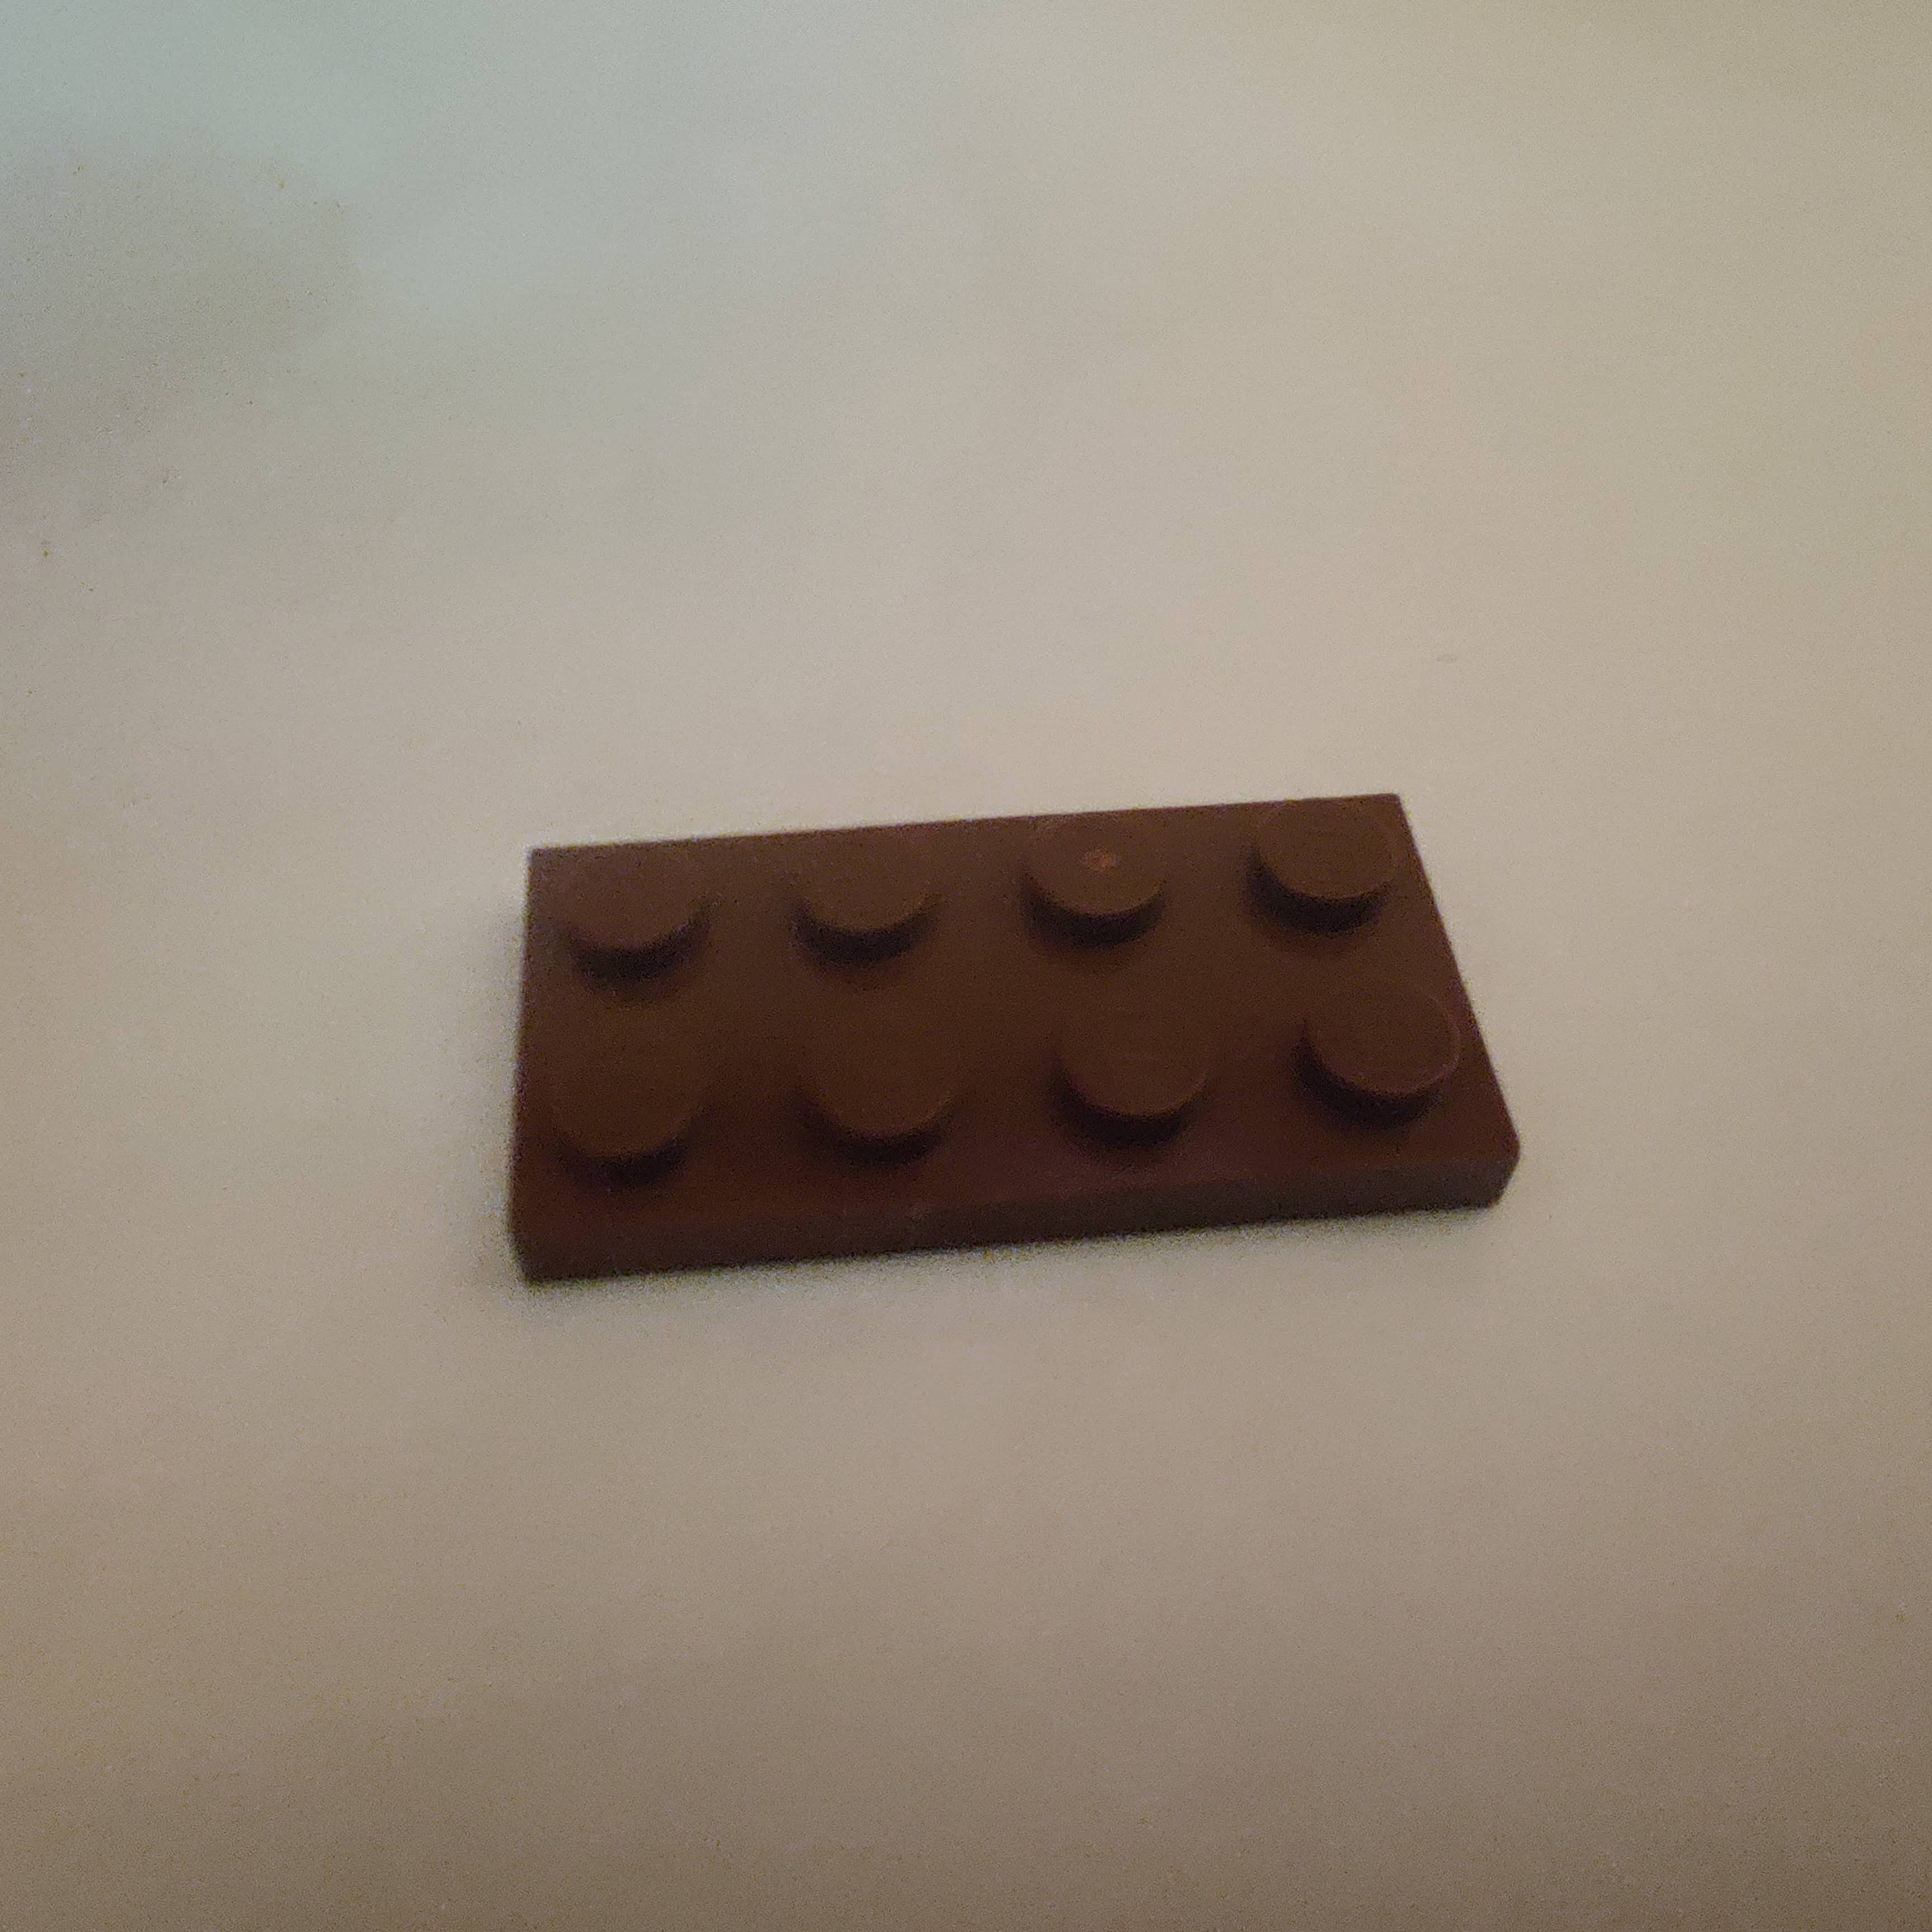
\includegraphics[width=\textwidth]{photographed images/2.jpg}
    \end{subfigure}
    \begin{subfigure}[b]{0.2\textwidth}
        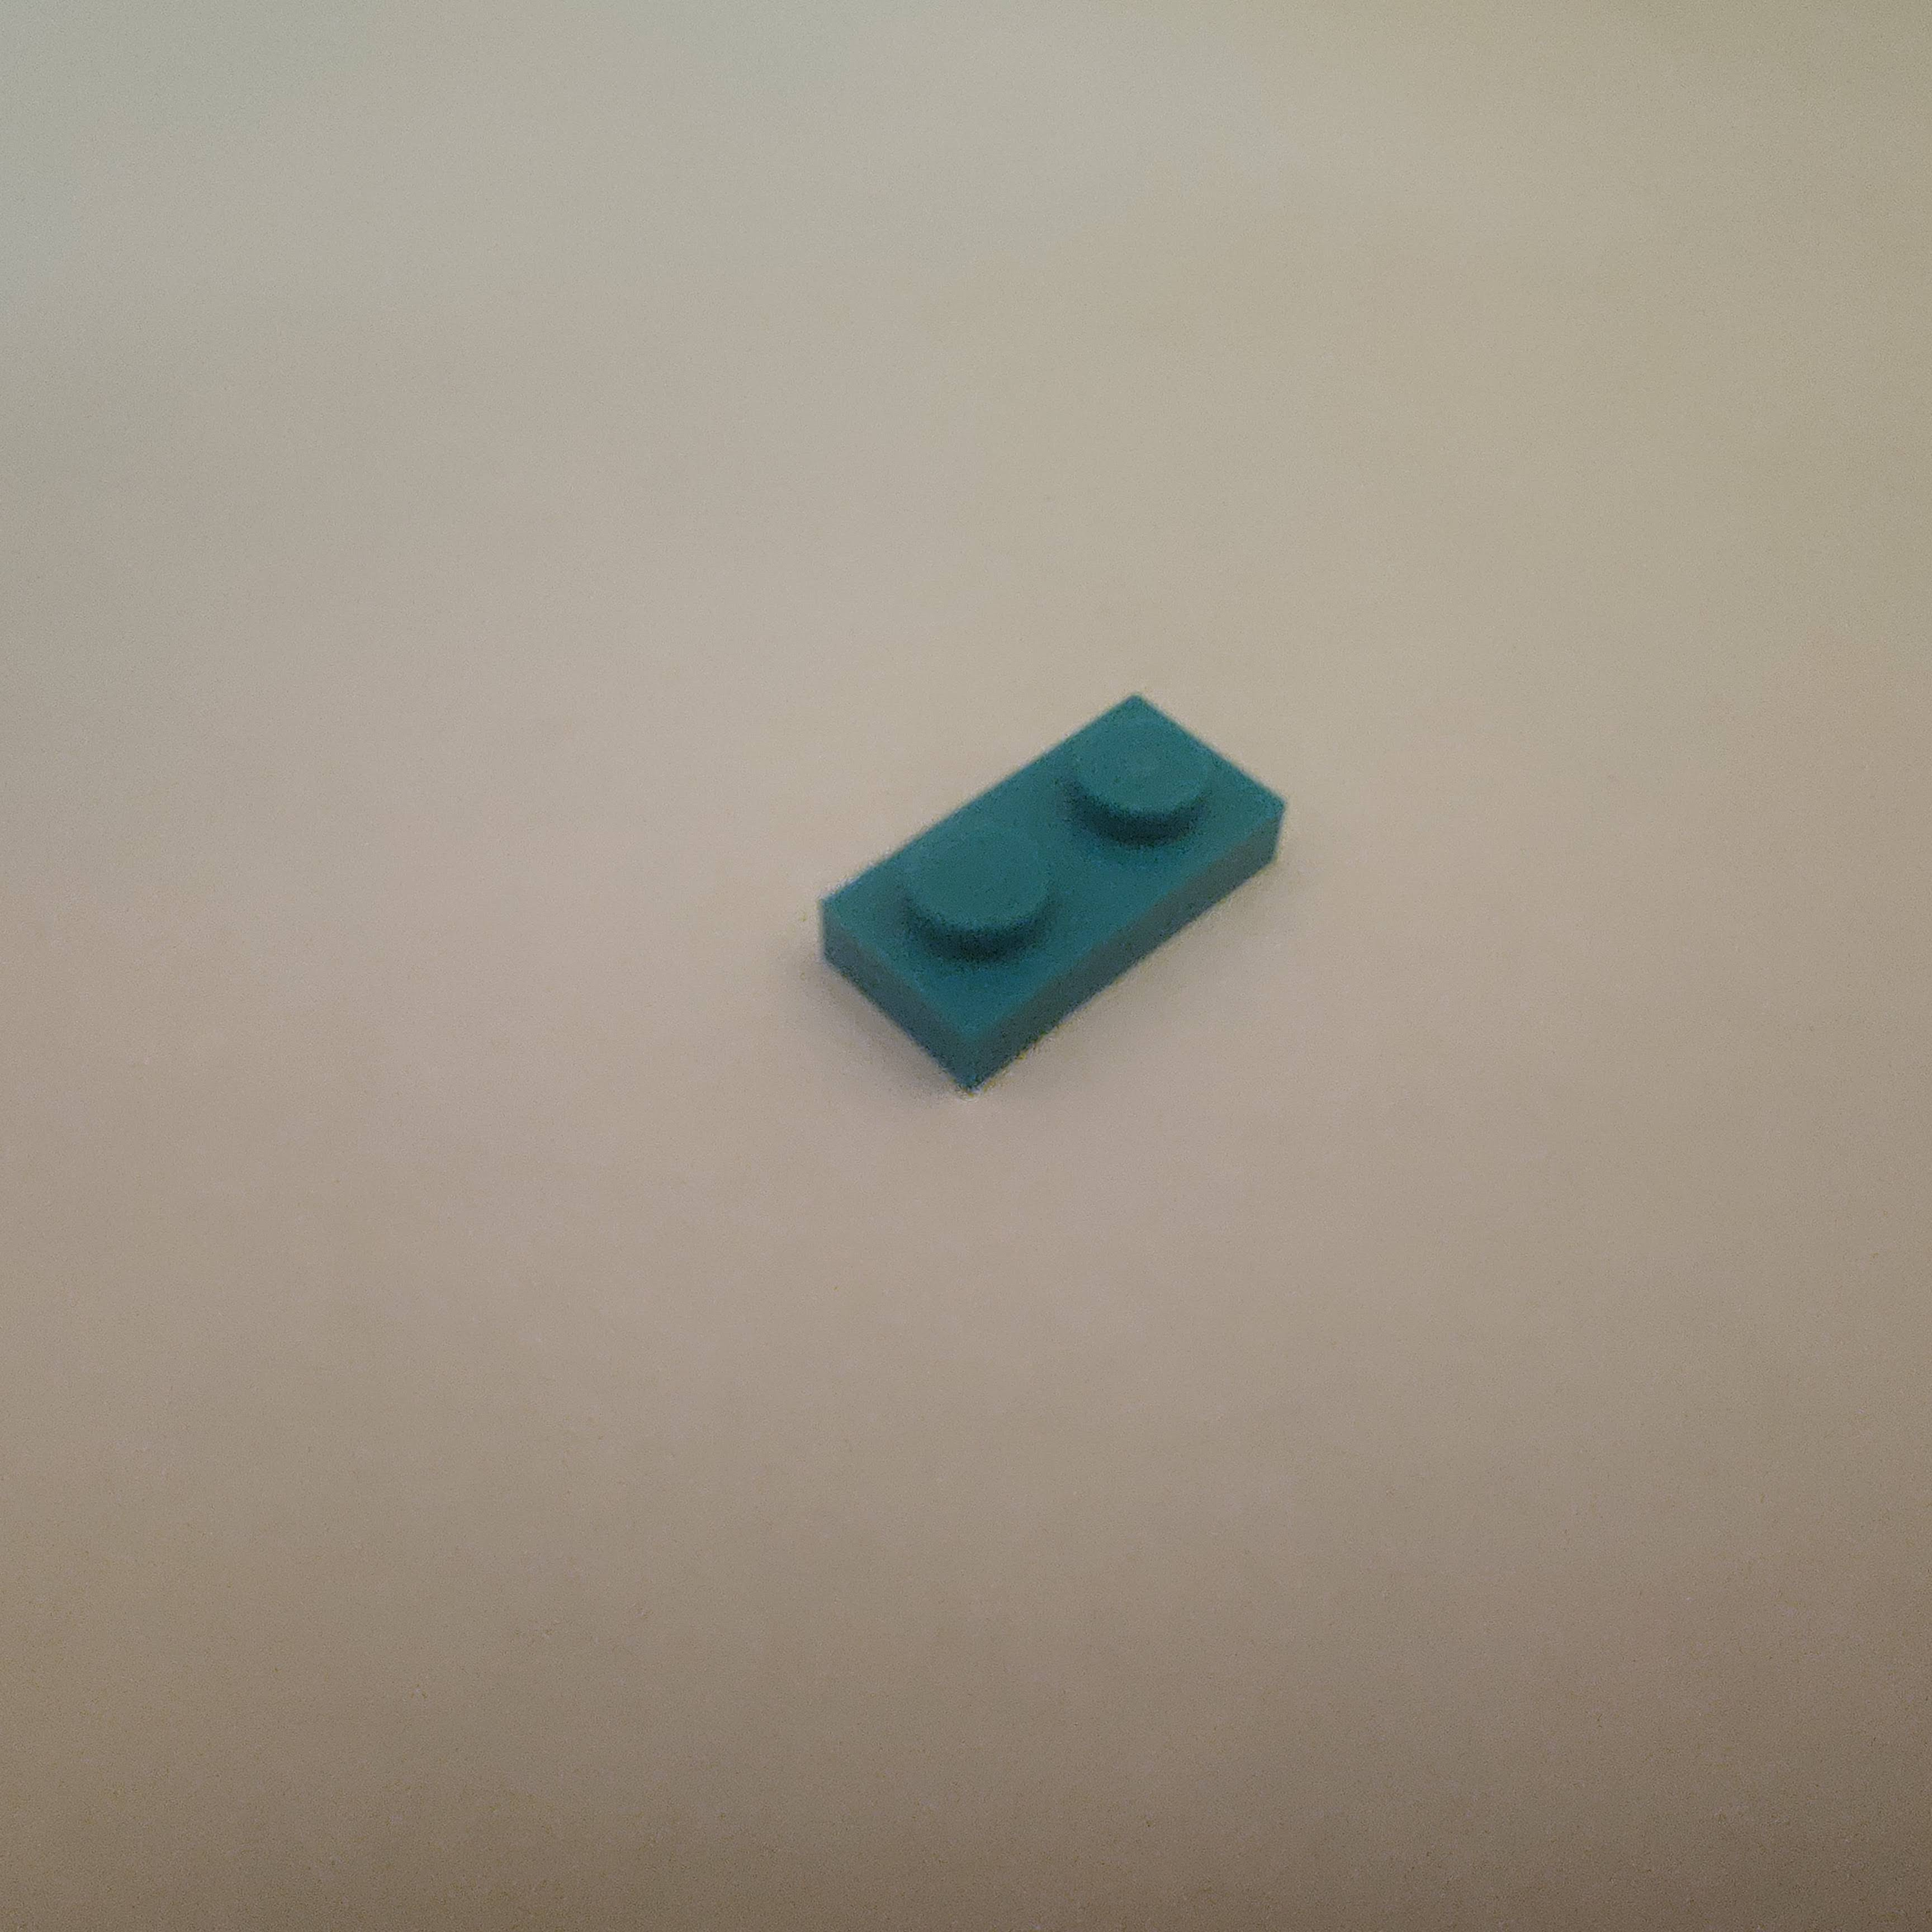
\includegraphics[width=\textwidth]{photographed images/3.jpg}
    \end{subfigure}
    \begin{subfigure}[b]{0.2\textwidth}
        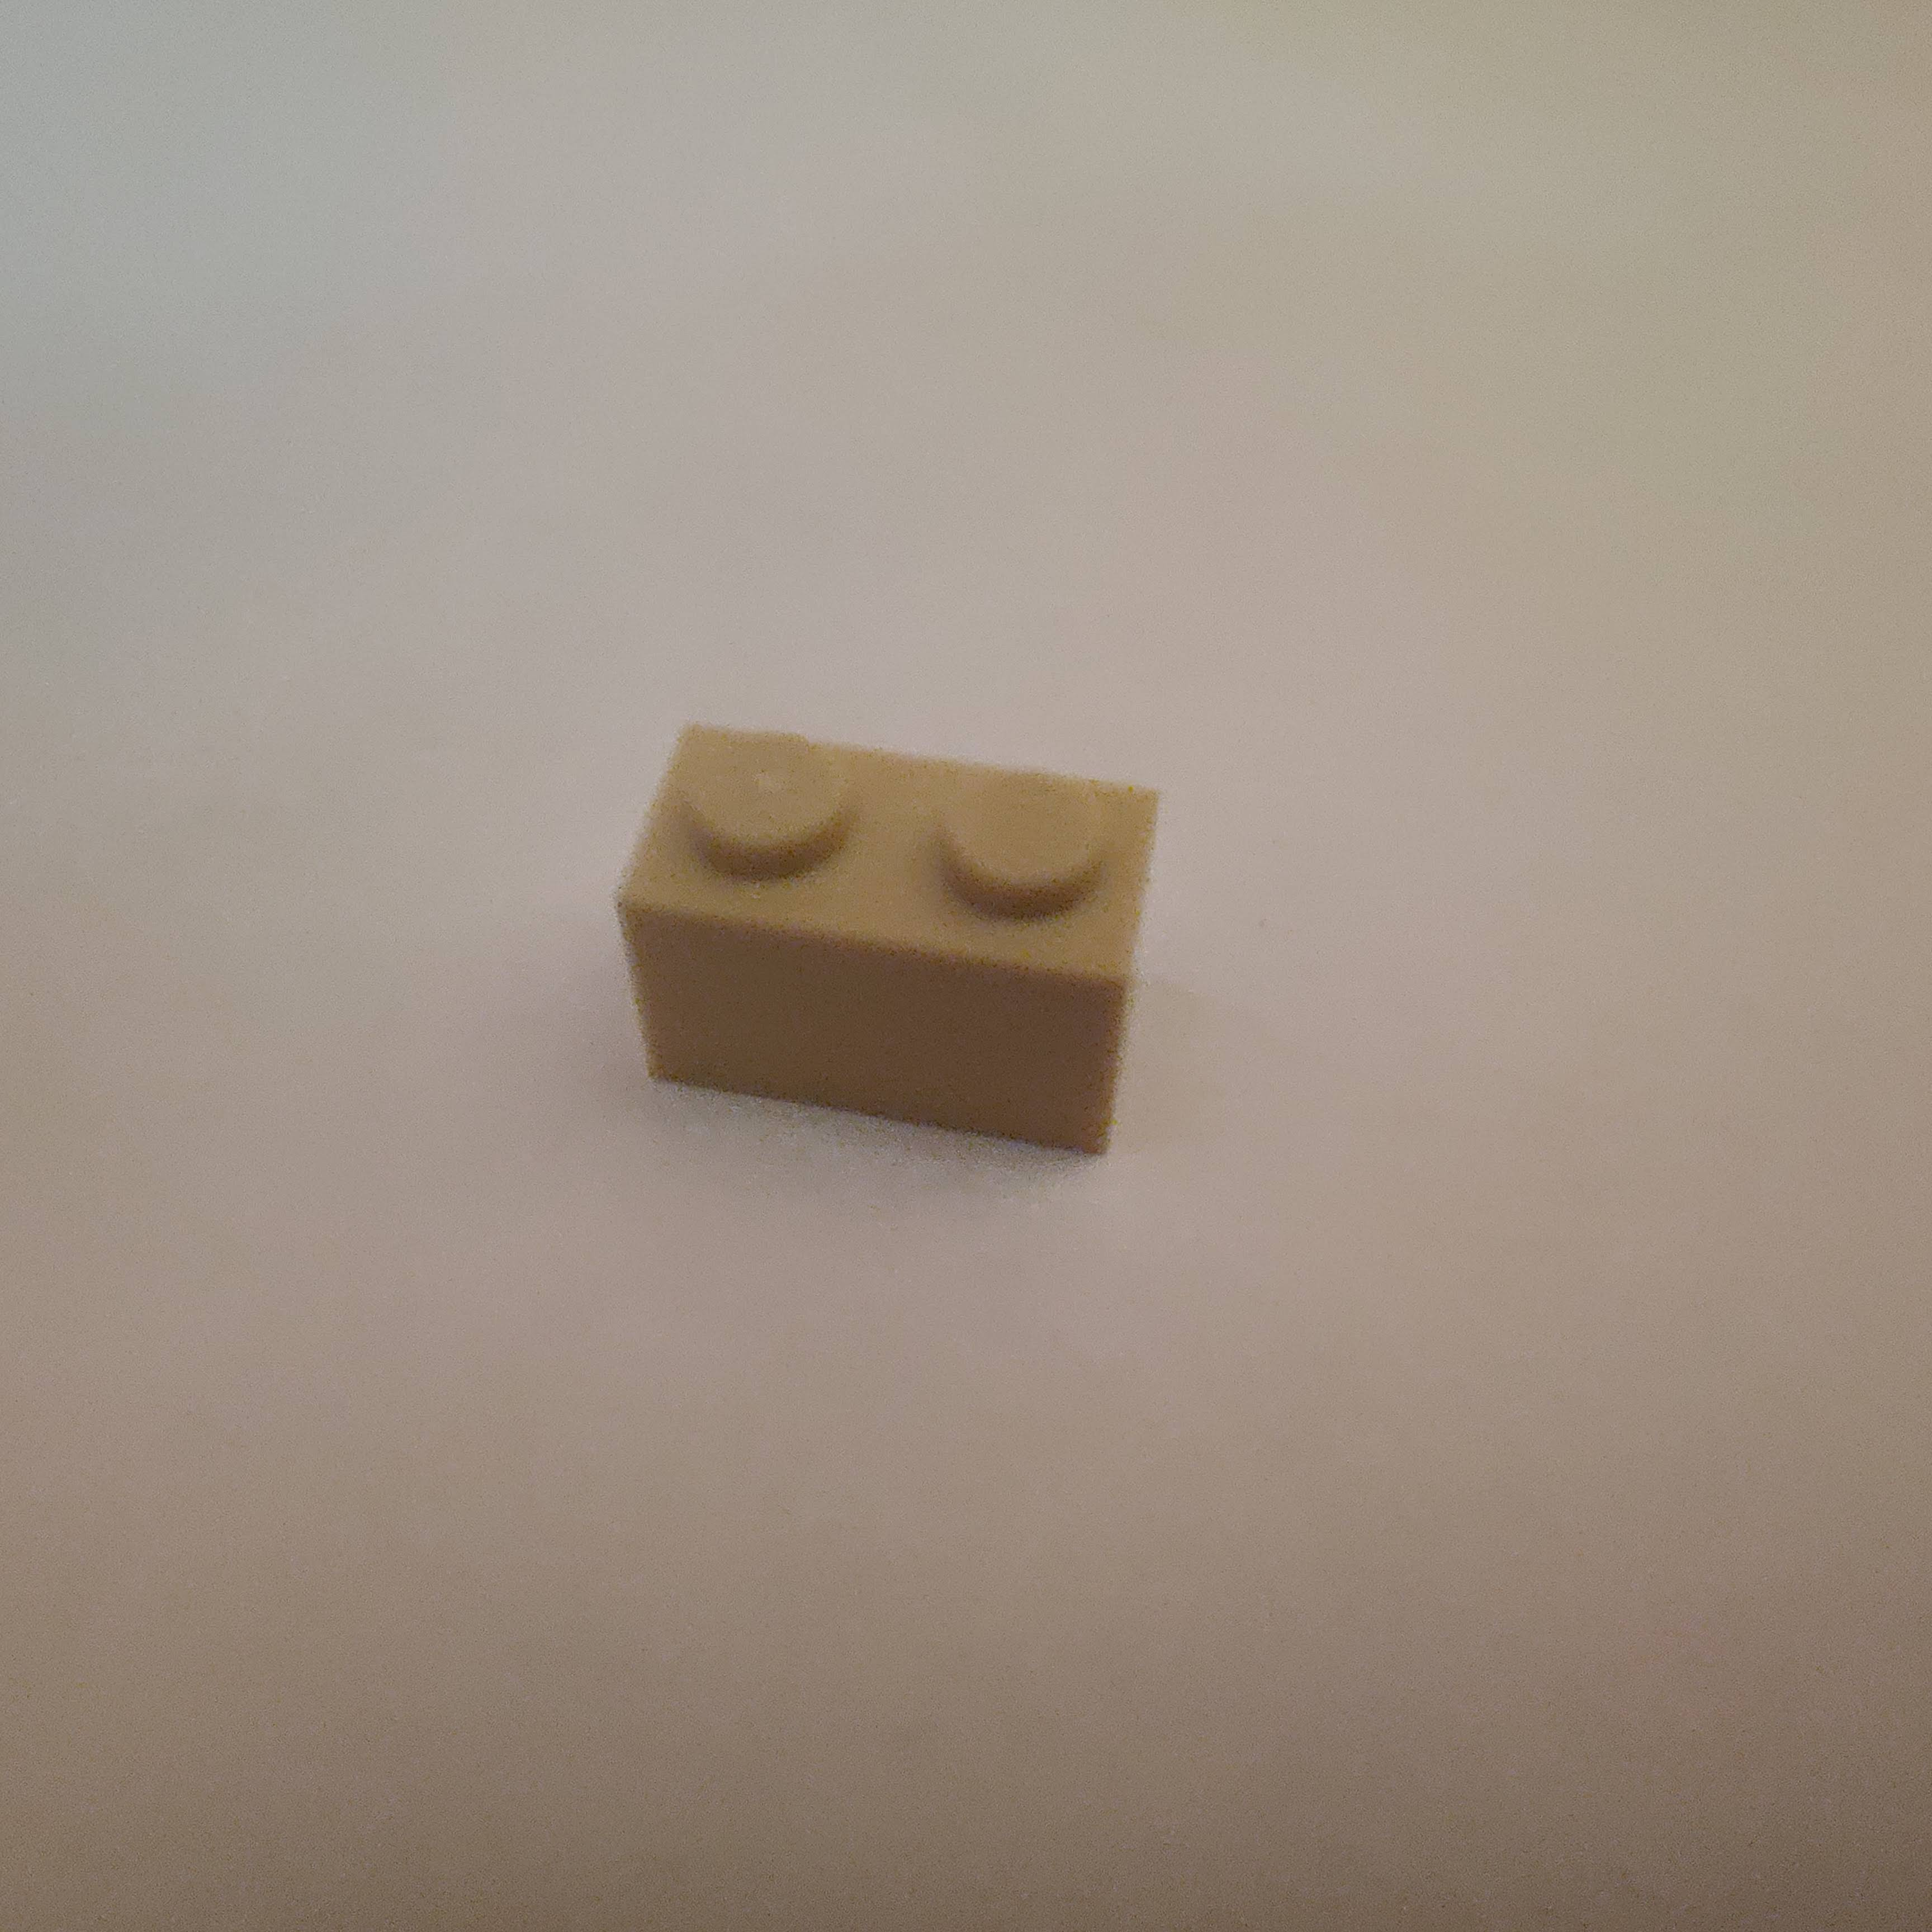
\includegraphics[width=\textwidth]{photographed images/4.jpg}
    \end{subfigure}
    \begin{subfigure}[b]{0.2\textwidth}
        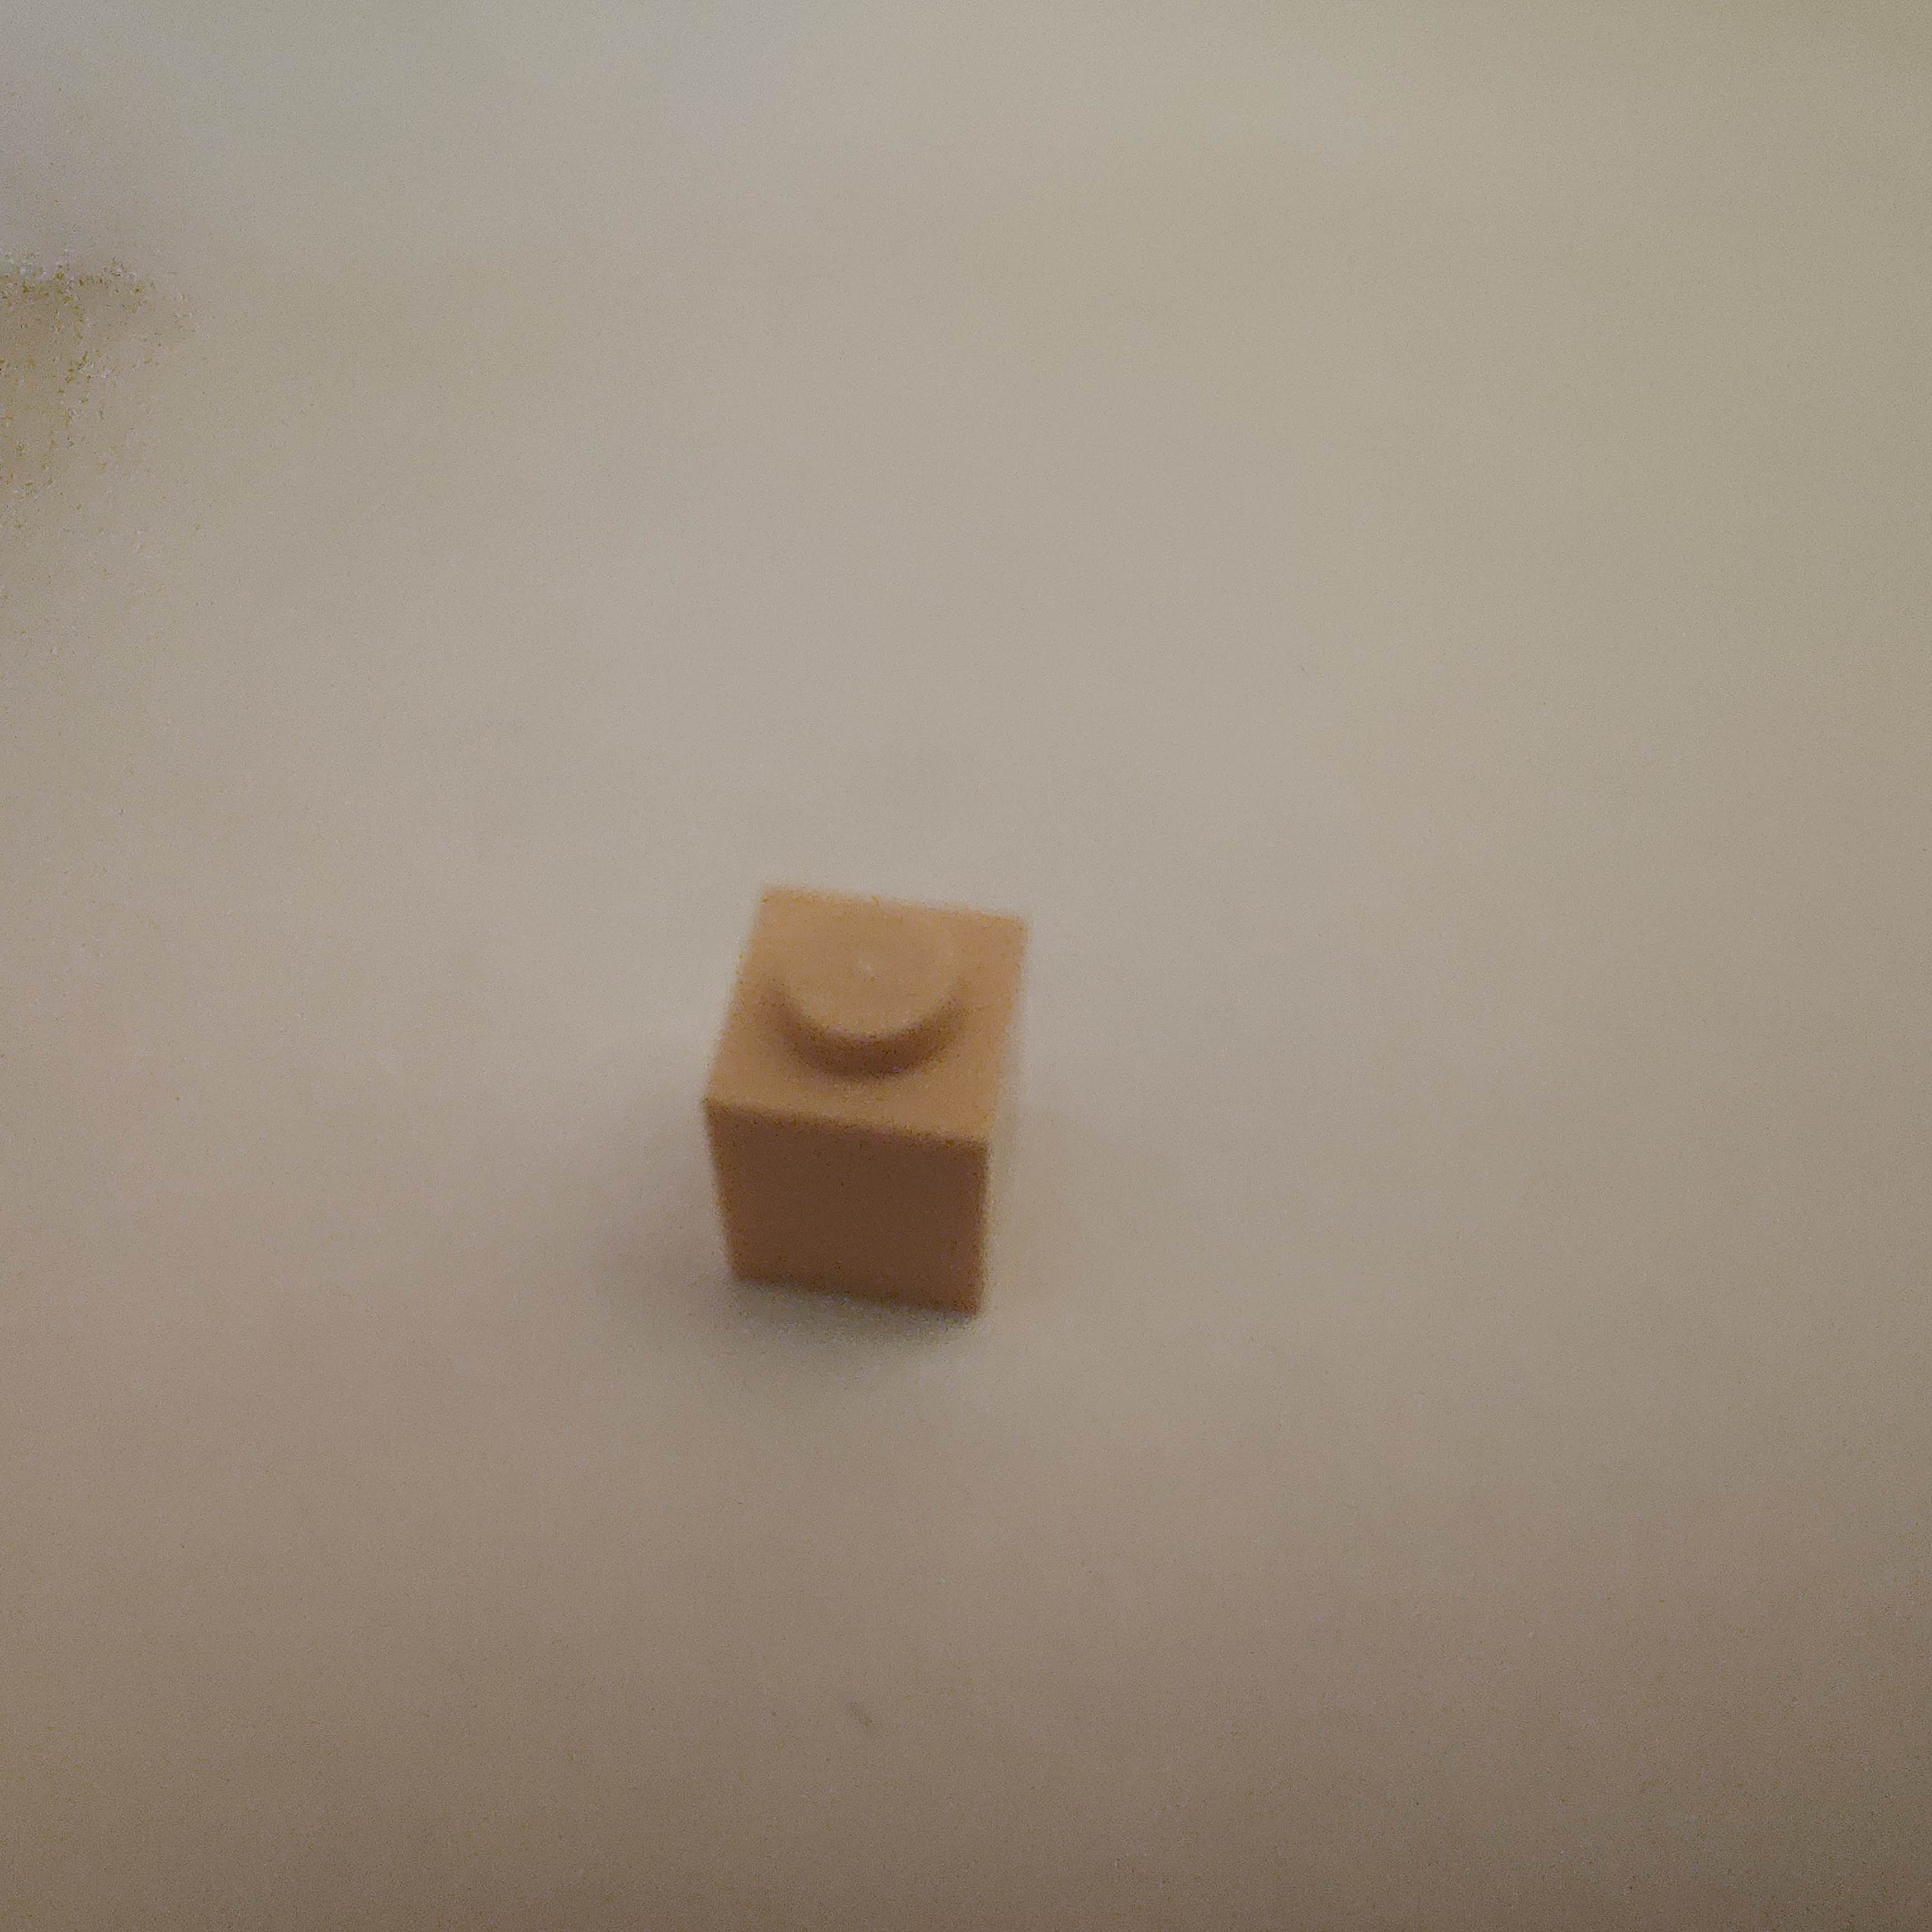
\includegraphics[width=\textwidth]{photographed images/5.jpg}
    \end{subfigure}
    \begin{subfigure}[b]{0.2\textwidth}
        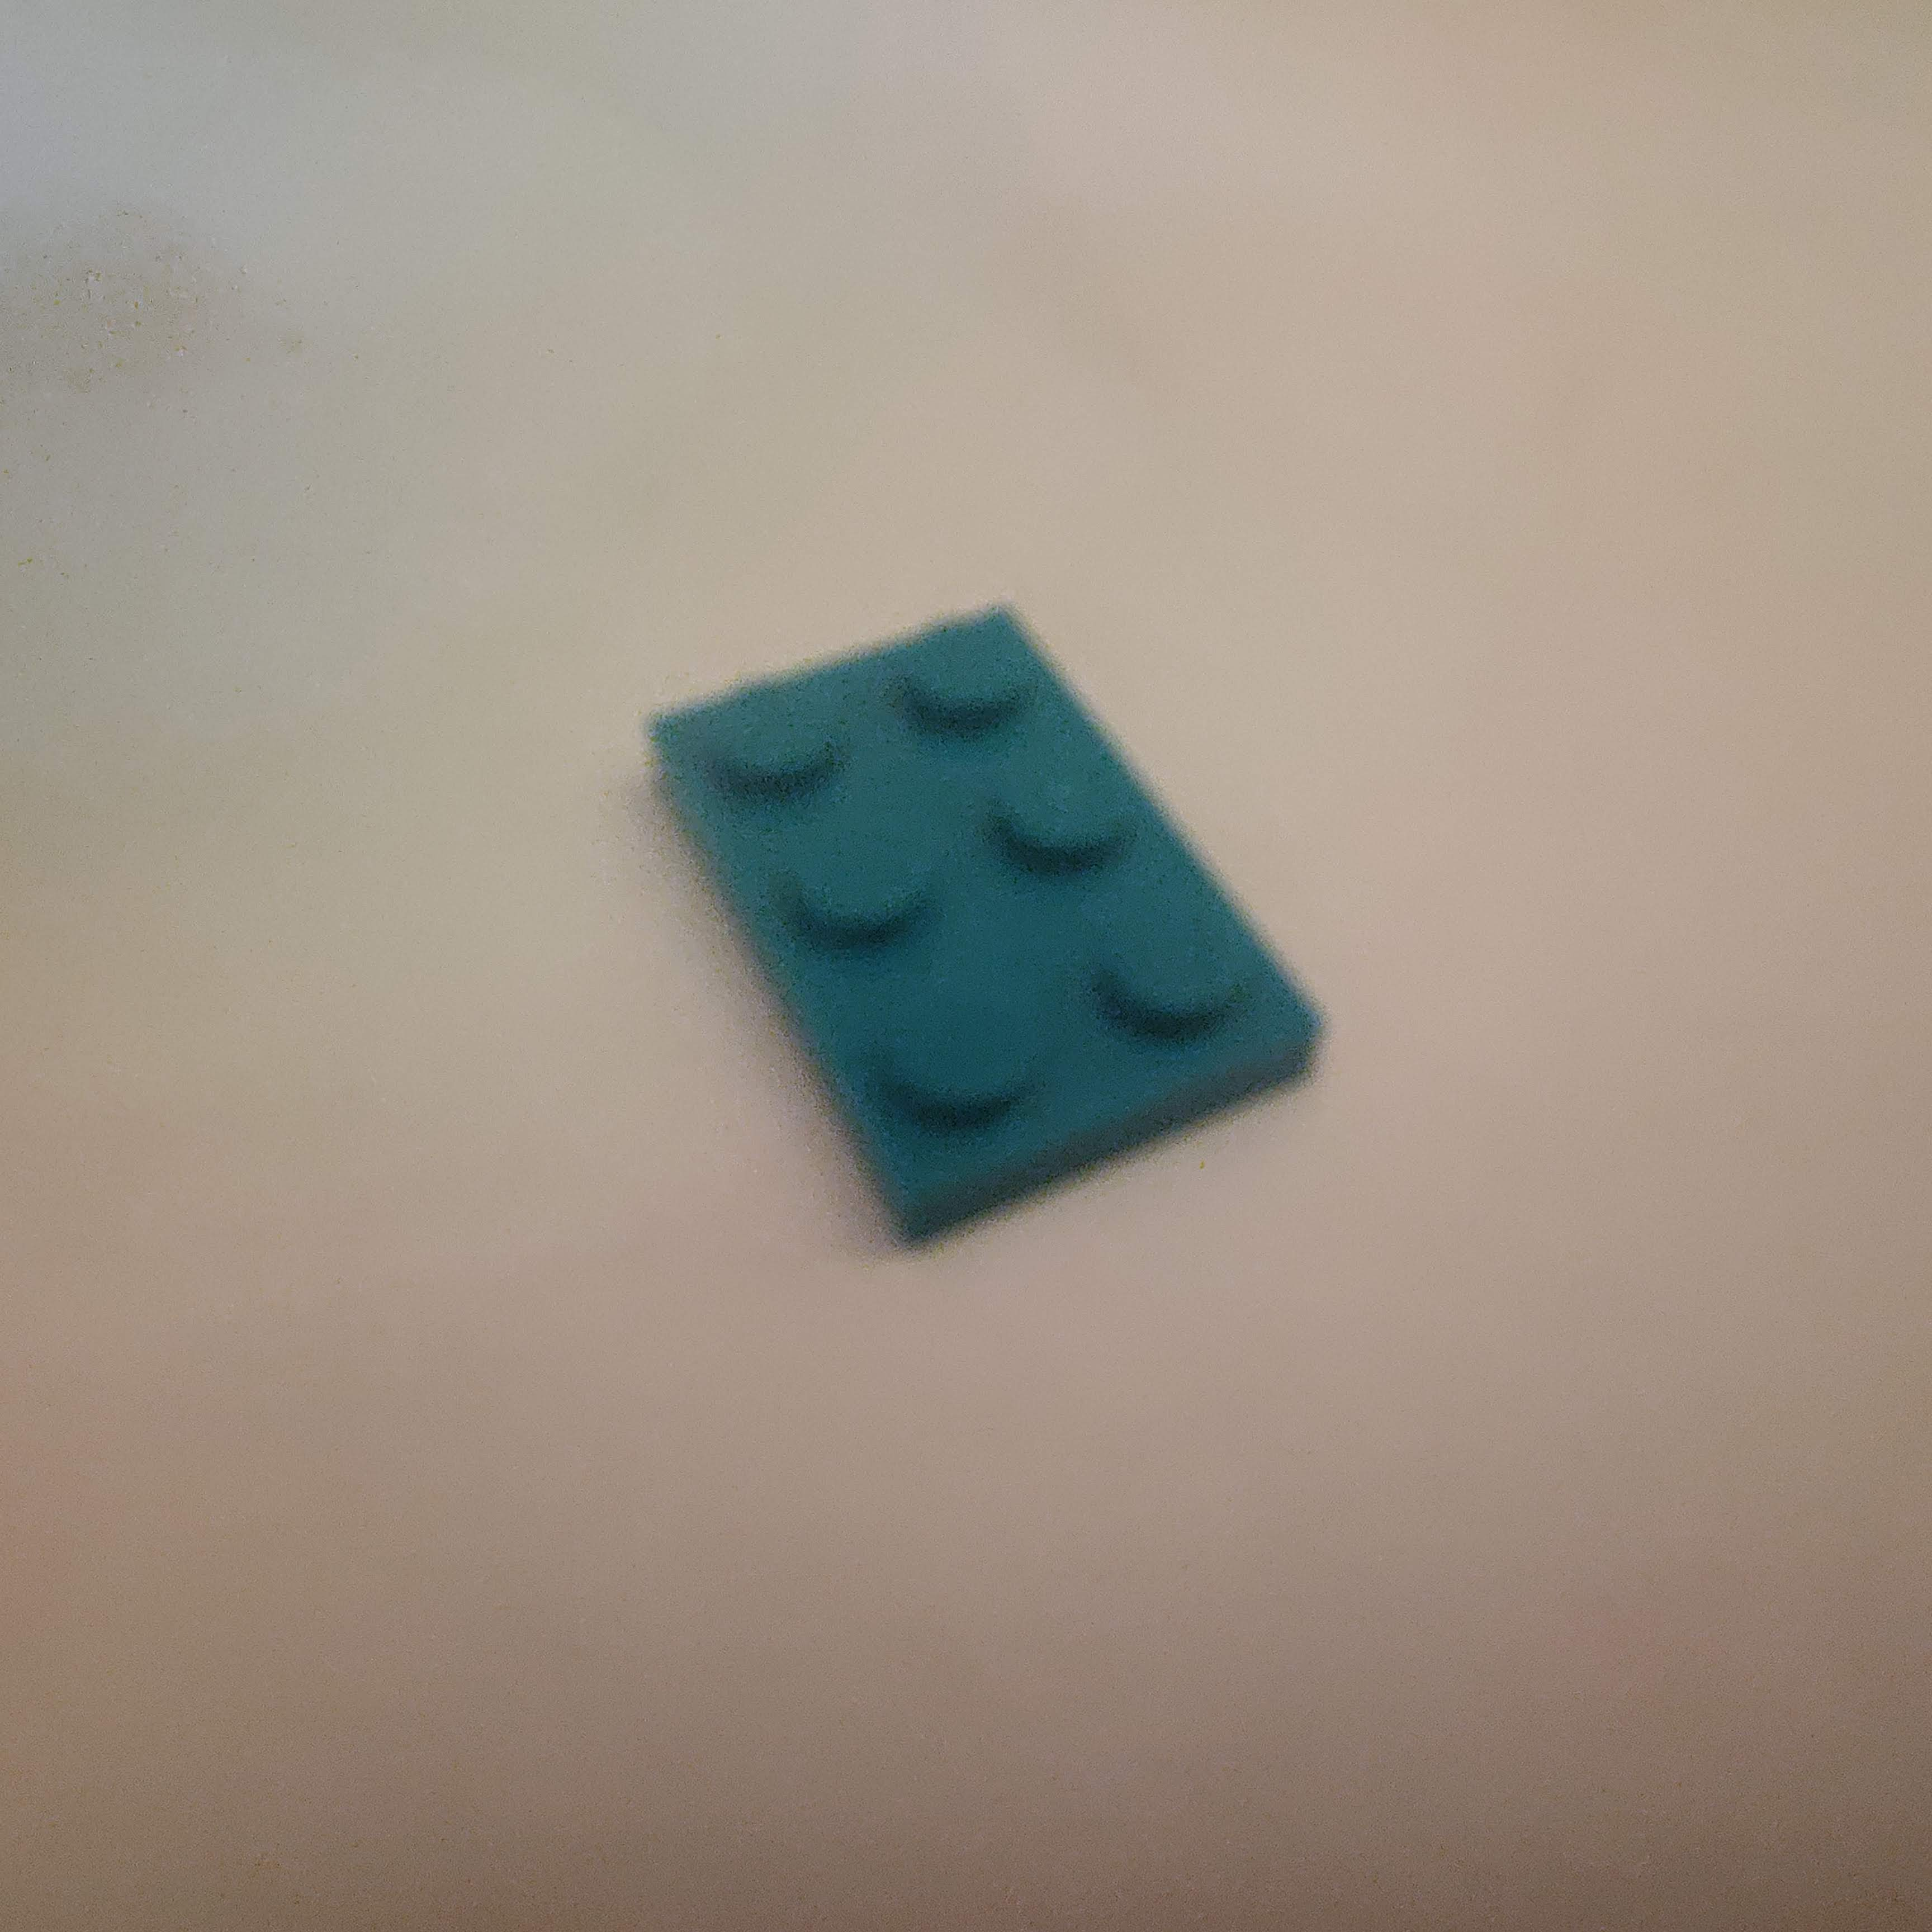
\includegraphics[width=\textwidth]{photographed images/6.jpg}
    \end{subfigure}
    \begin{subfigure}[b]{0.2\textwidth}
        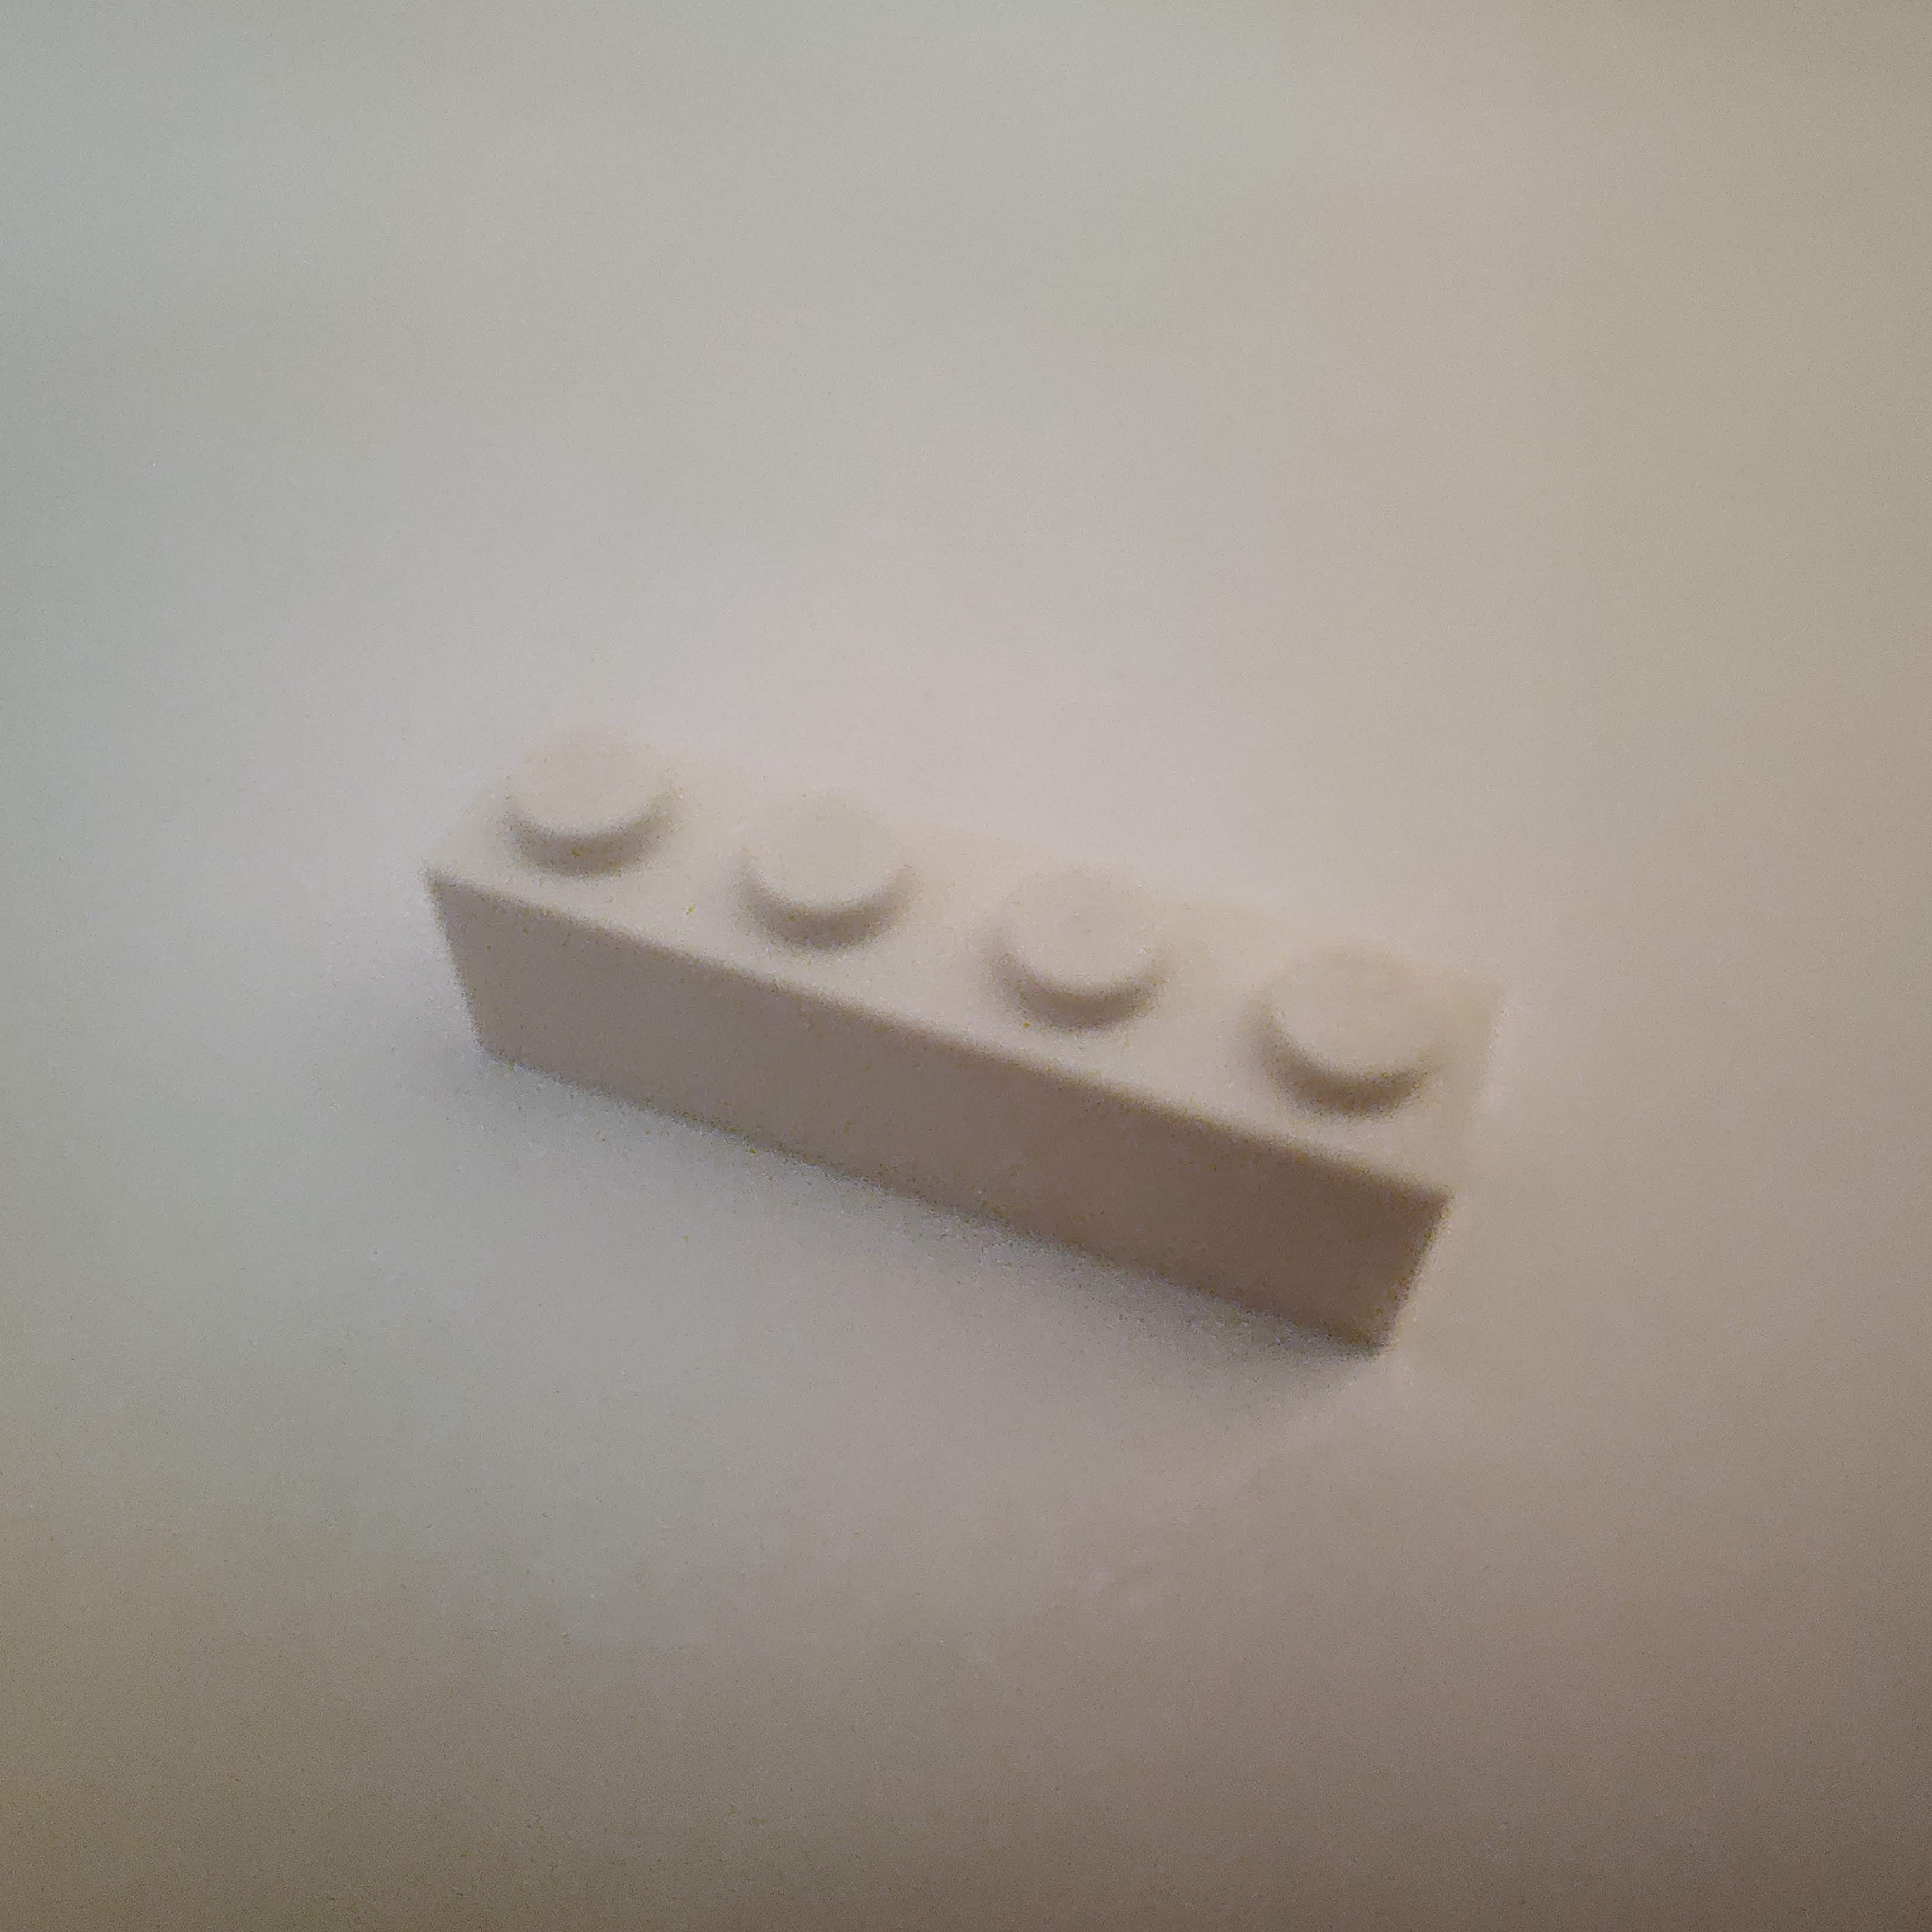
\includegraphics[width=\textwidth]{photographed images/7.jpg}
    \end{subfigure}
    \begin{subfigure}[b]{0.2\textwidth}
        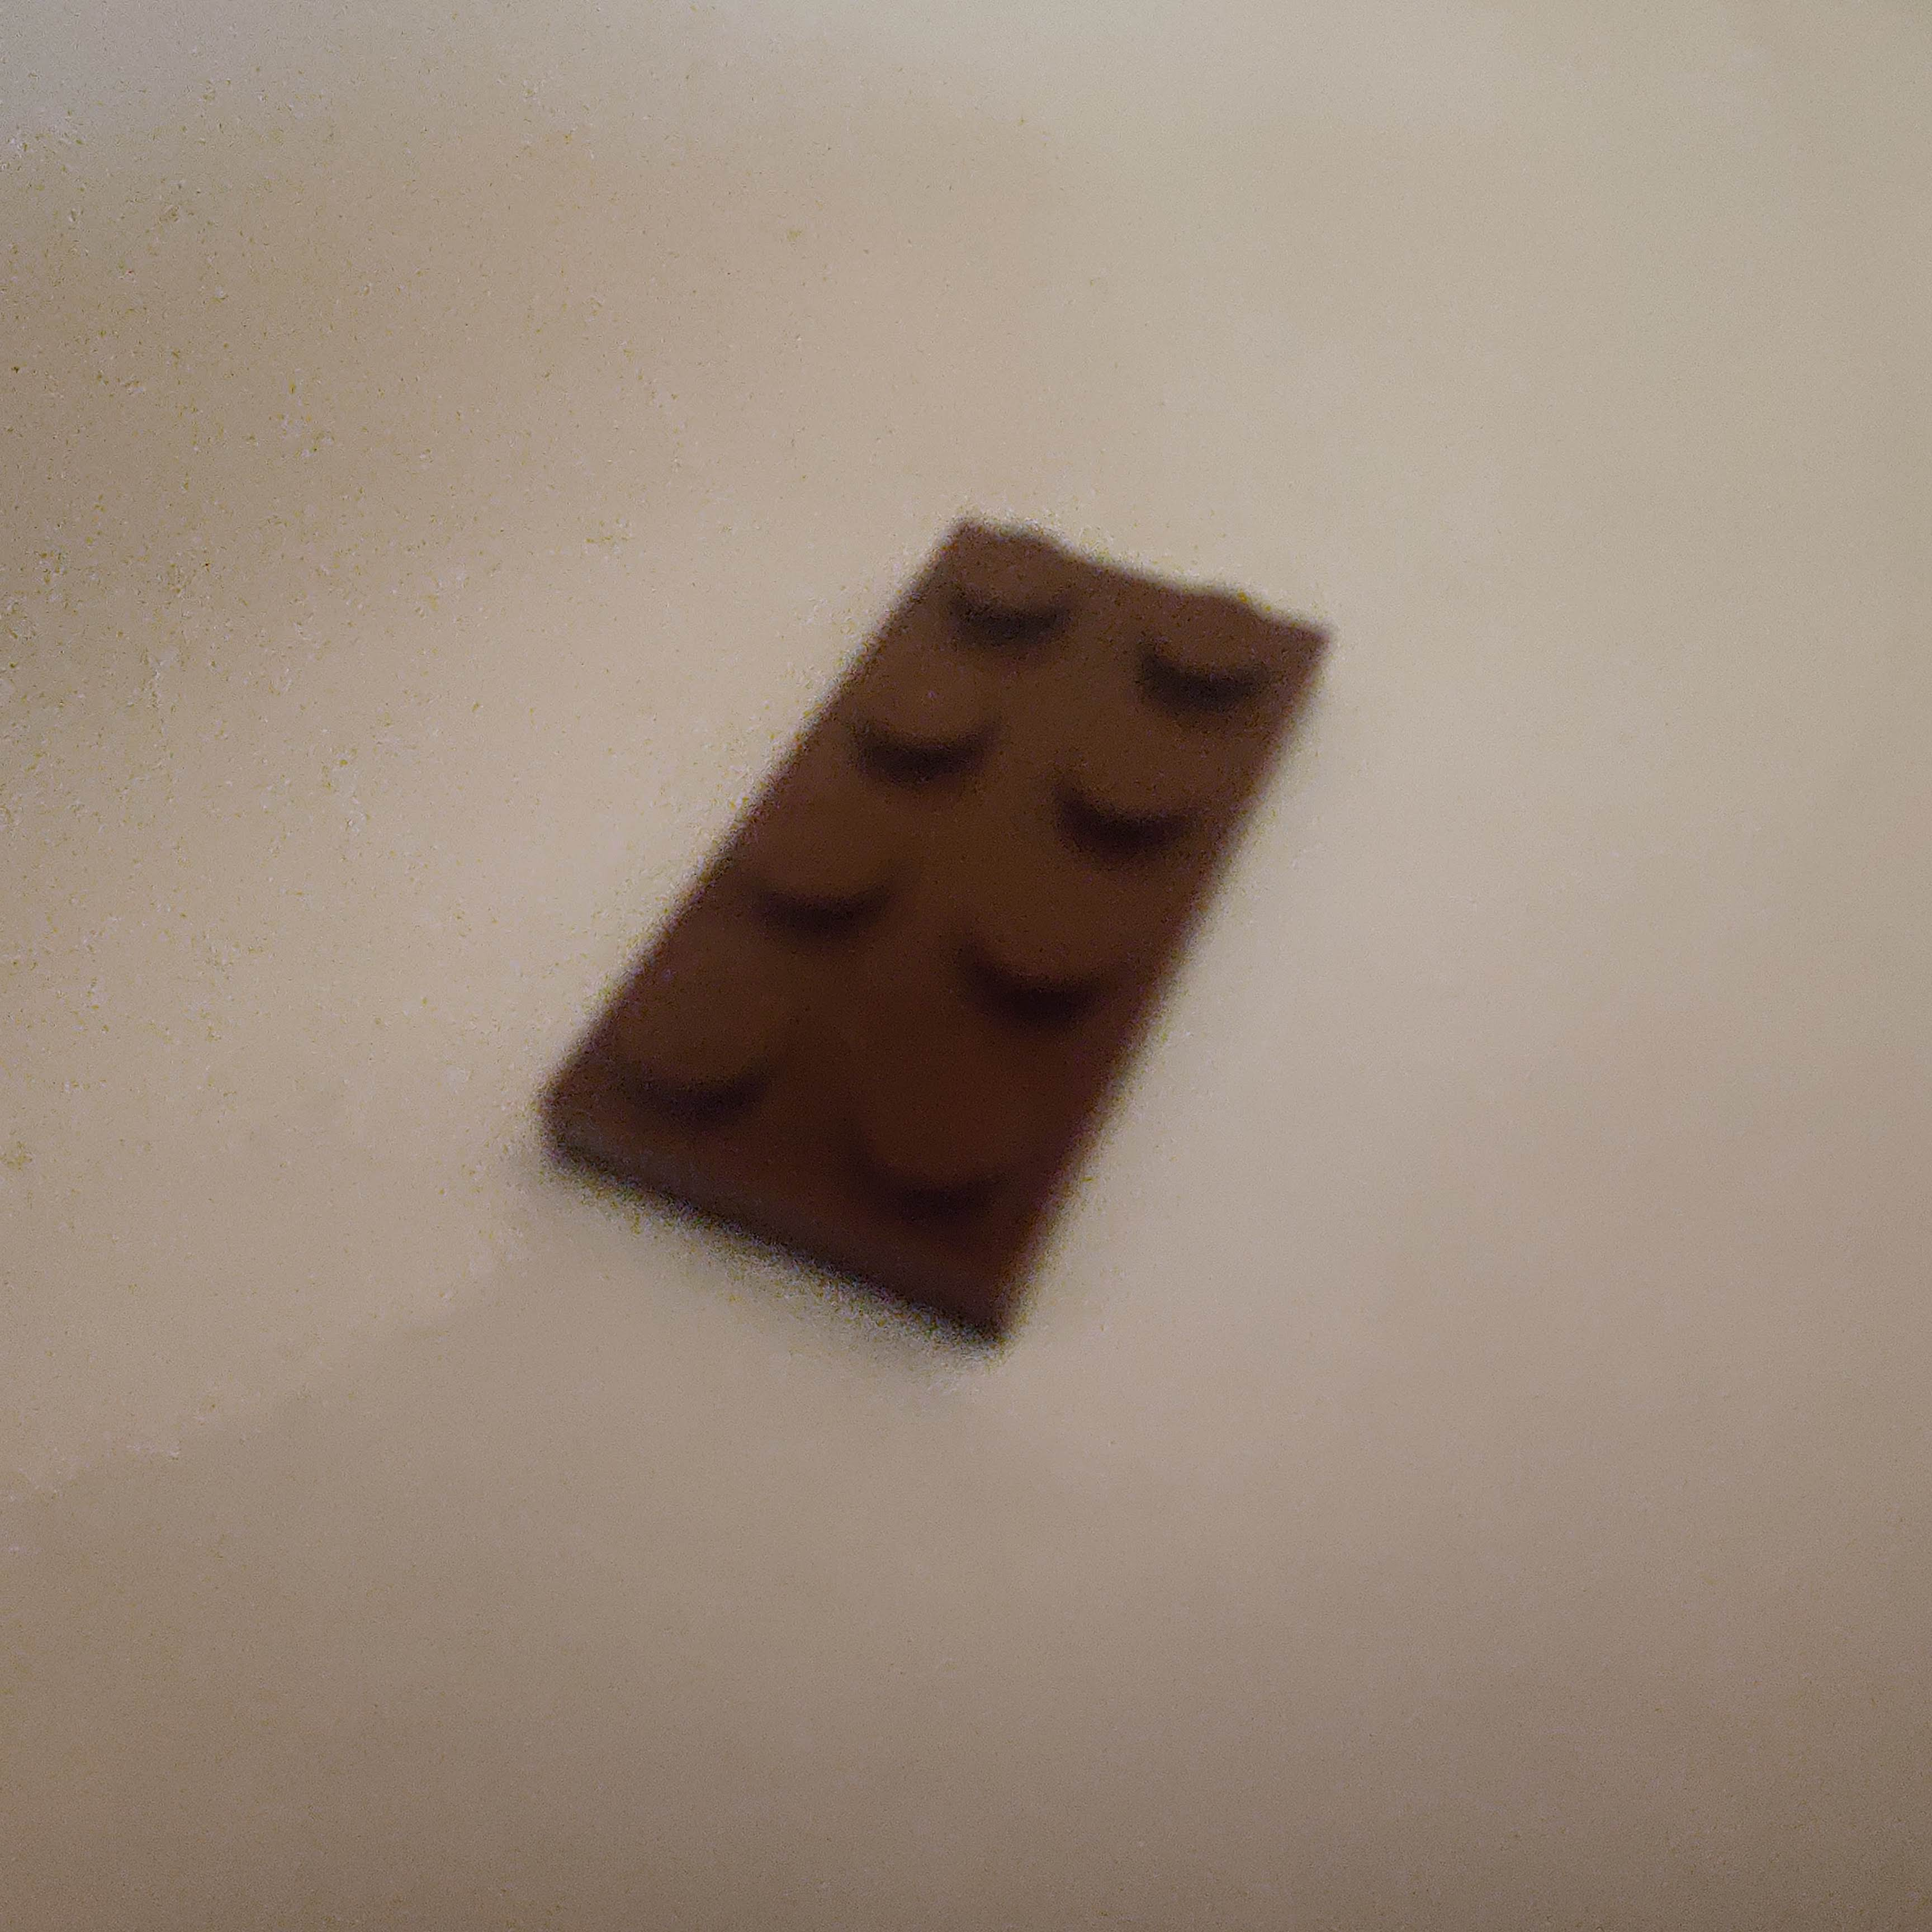
\includegraphics[width=\textwidth]{photographed images/8.jpg}
    \end{subfigure}
    \begin{subfigure}[b]{0.2\textwidth}
        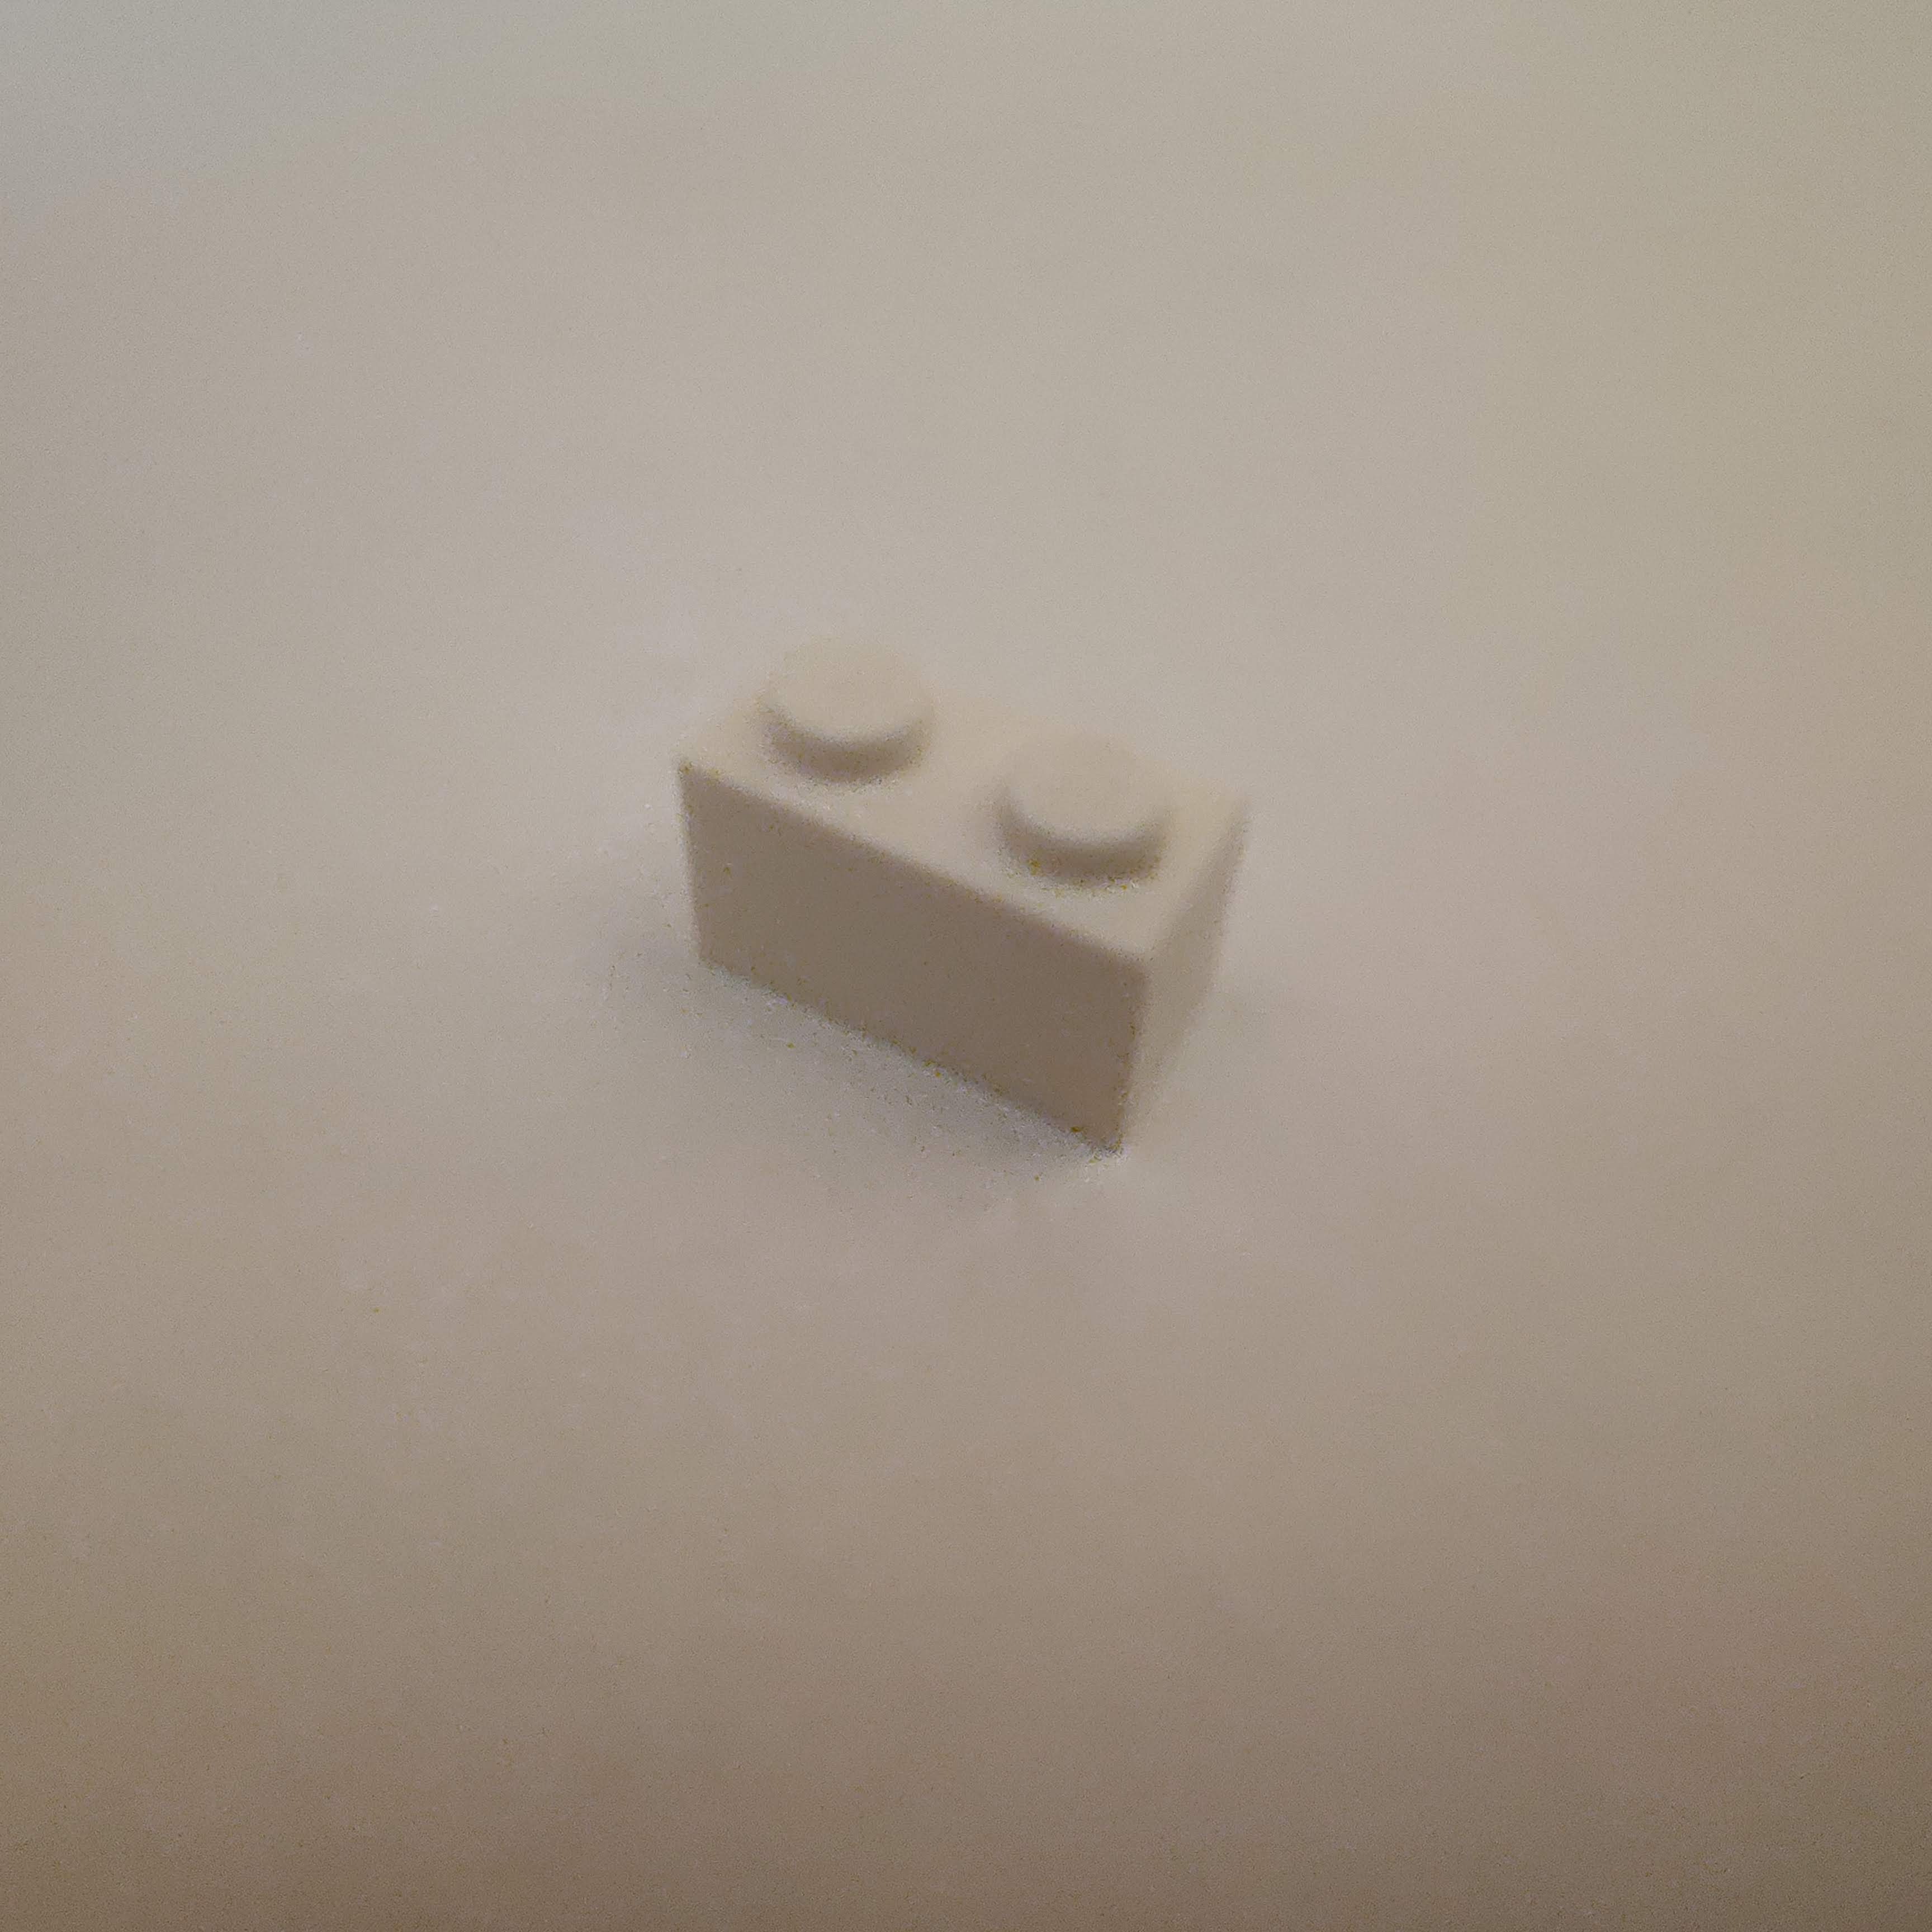
\includegraphics[width=\textwidth]{photographed images/9.jpg}
    \end{subfigure}
    \begin{subfigure}[b]{0.2\textwidth}
        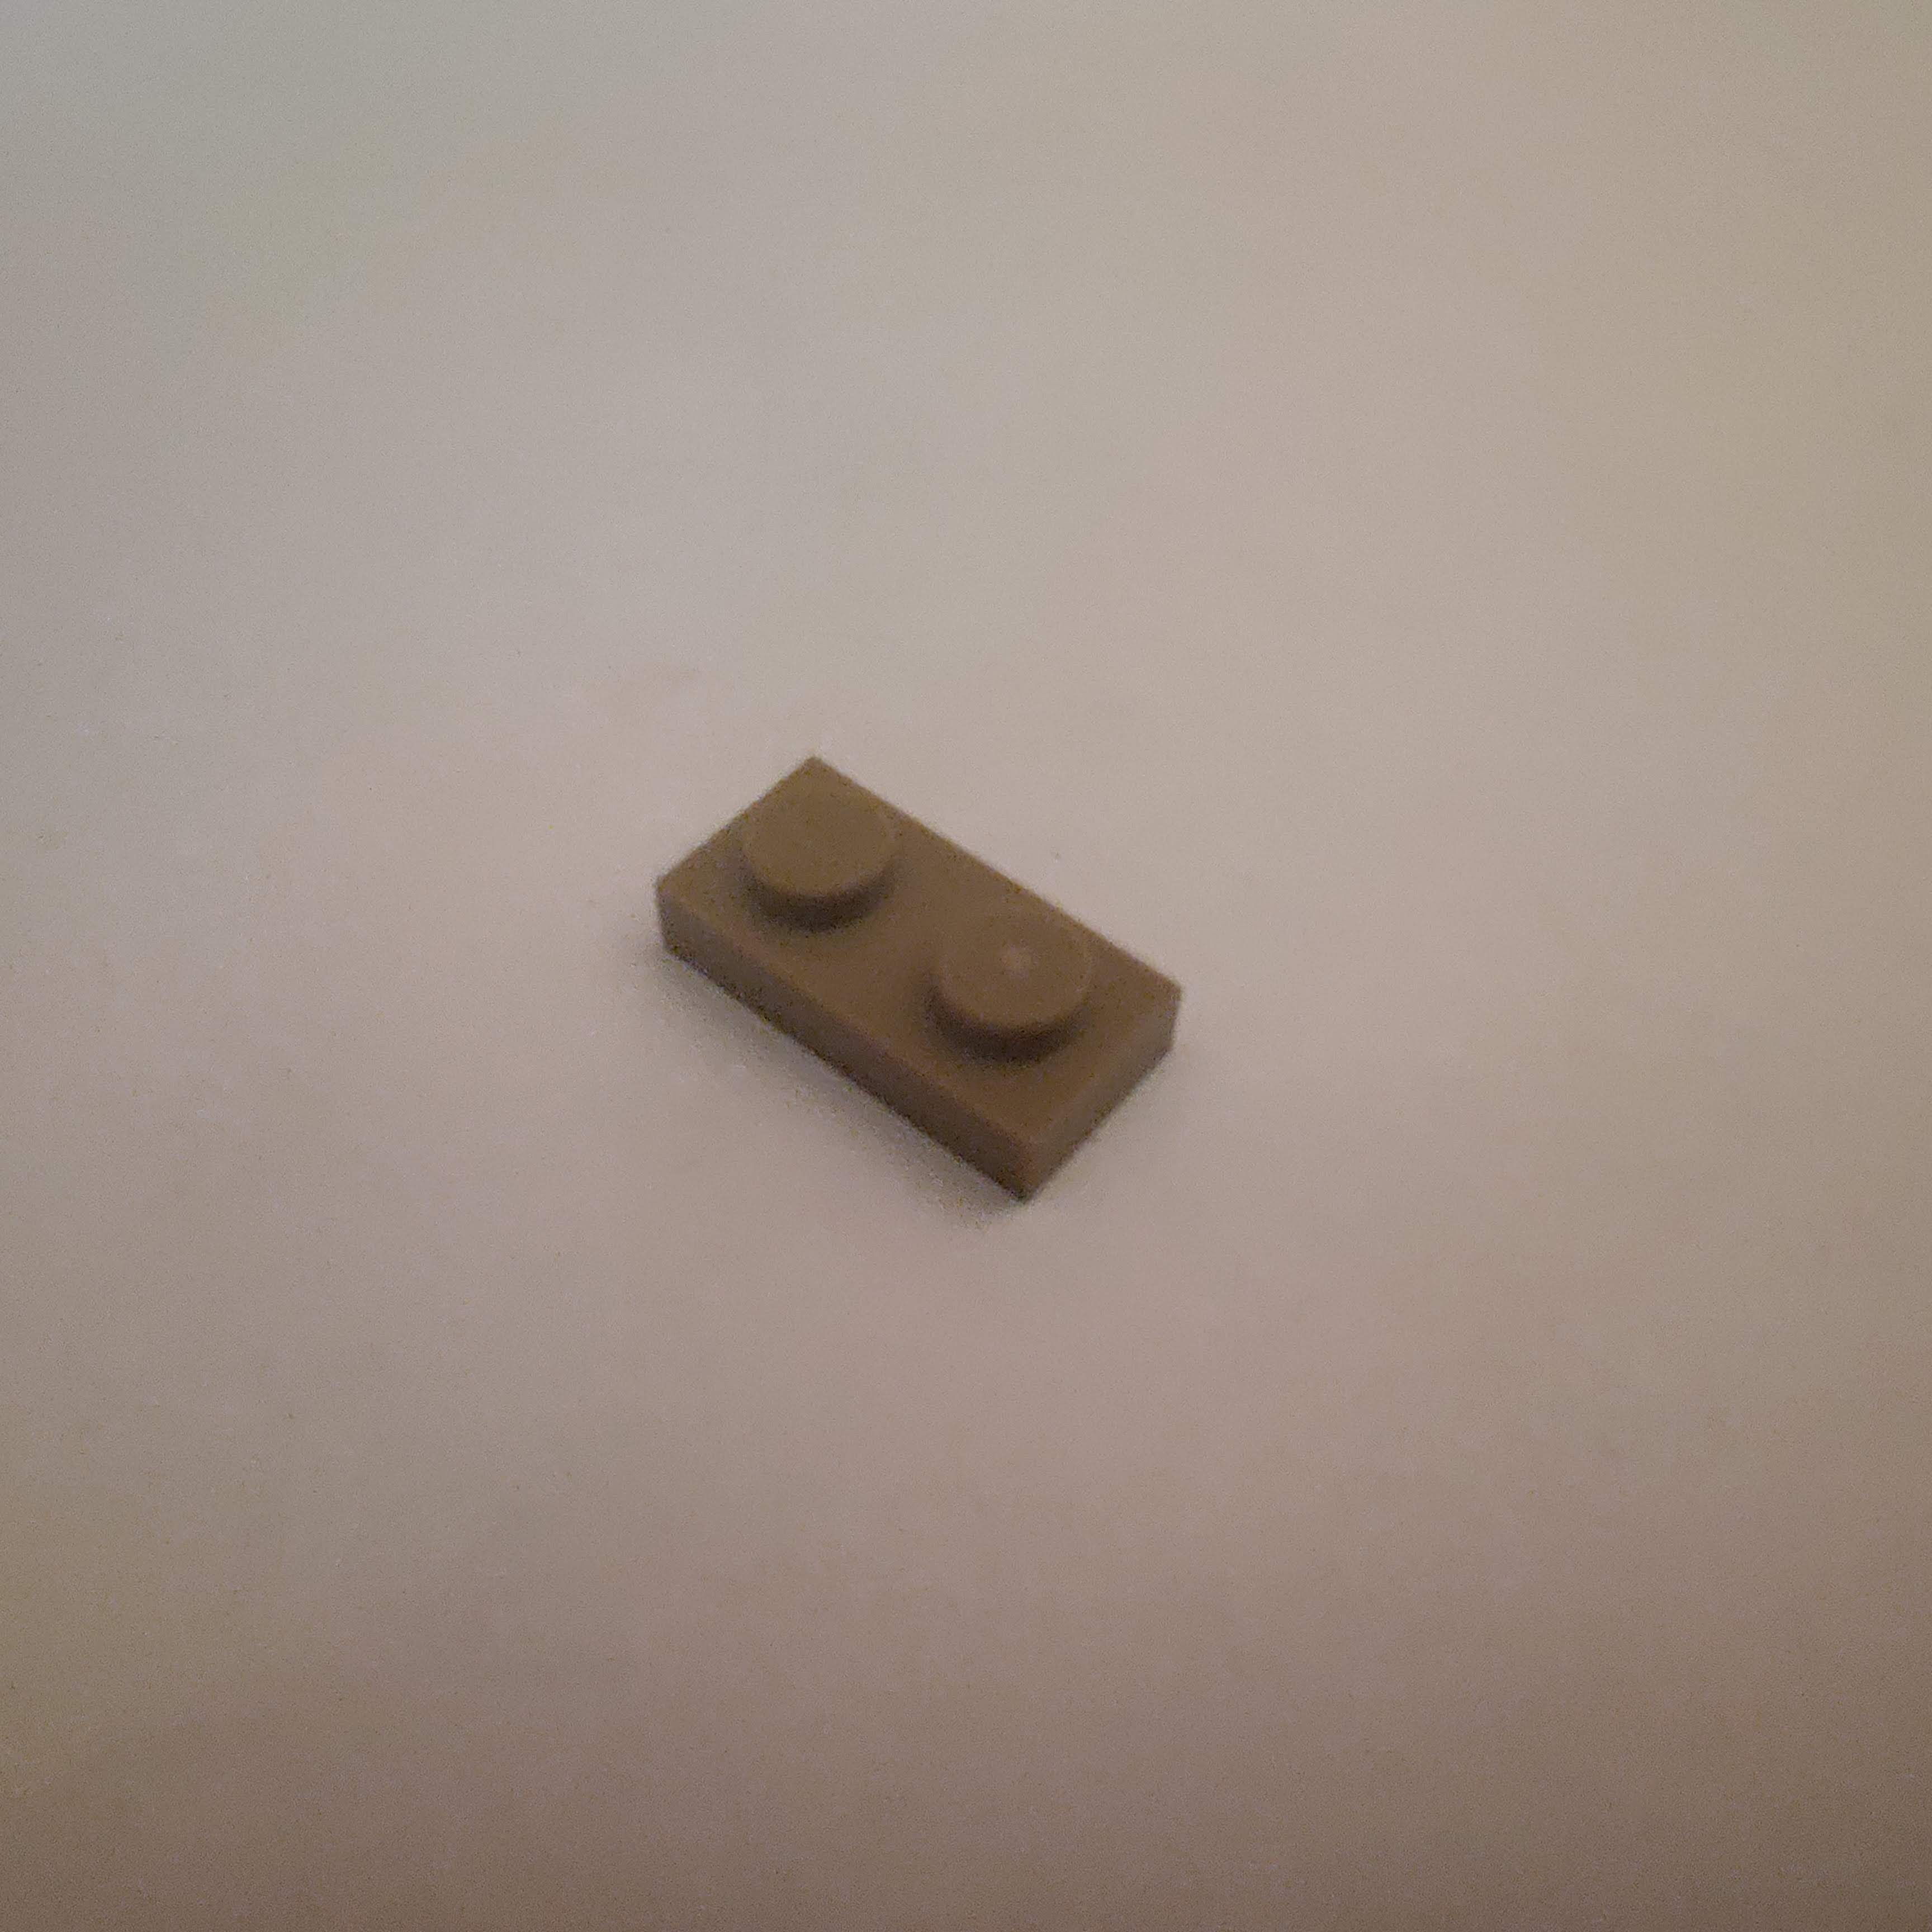
\includegraphics[width=\textwidth]{photographed images/10.jpg}
    \end{subfigure}
    \begin{subfigure}[b]{0.2\textwidth}
        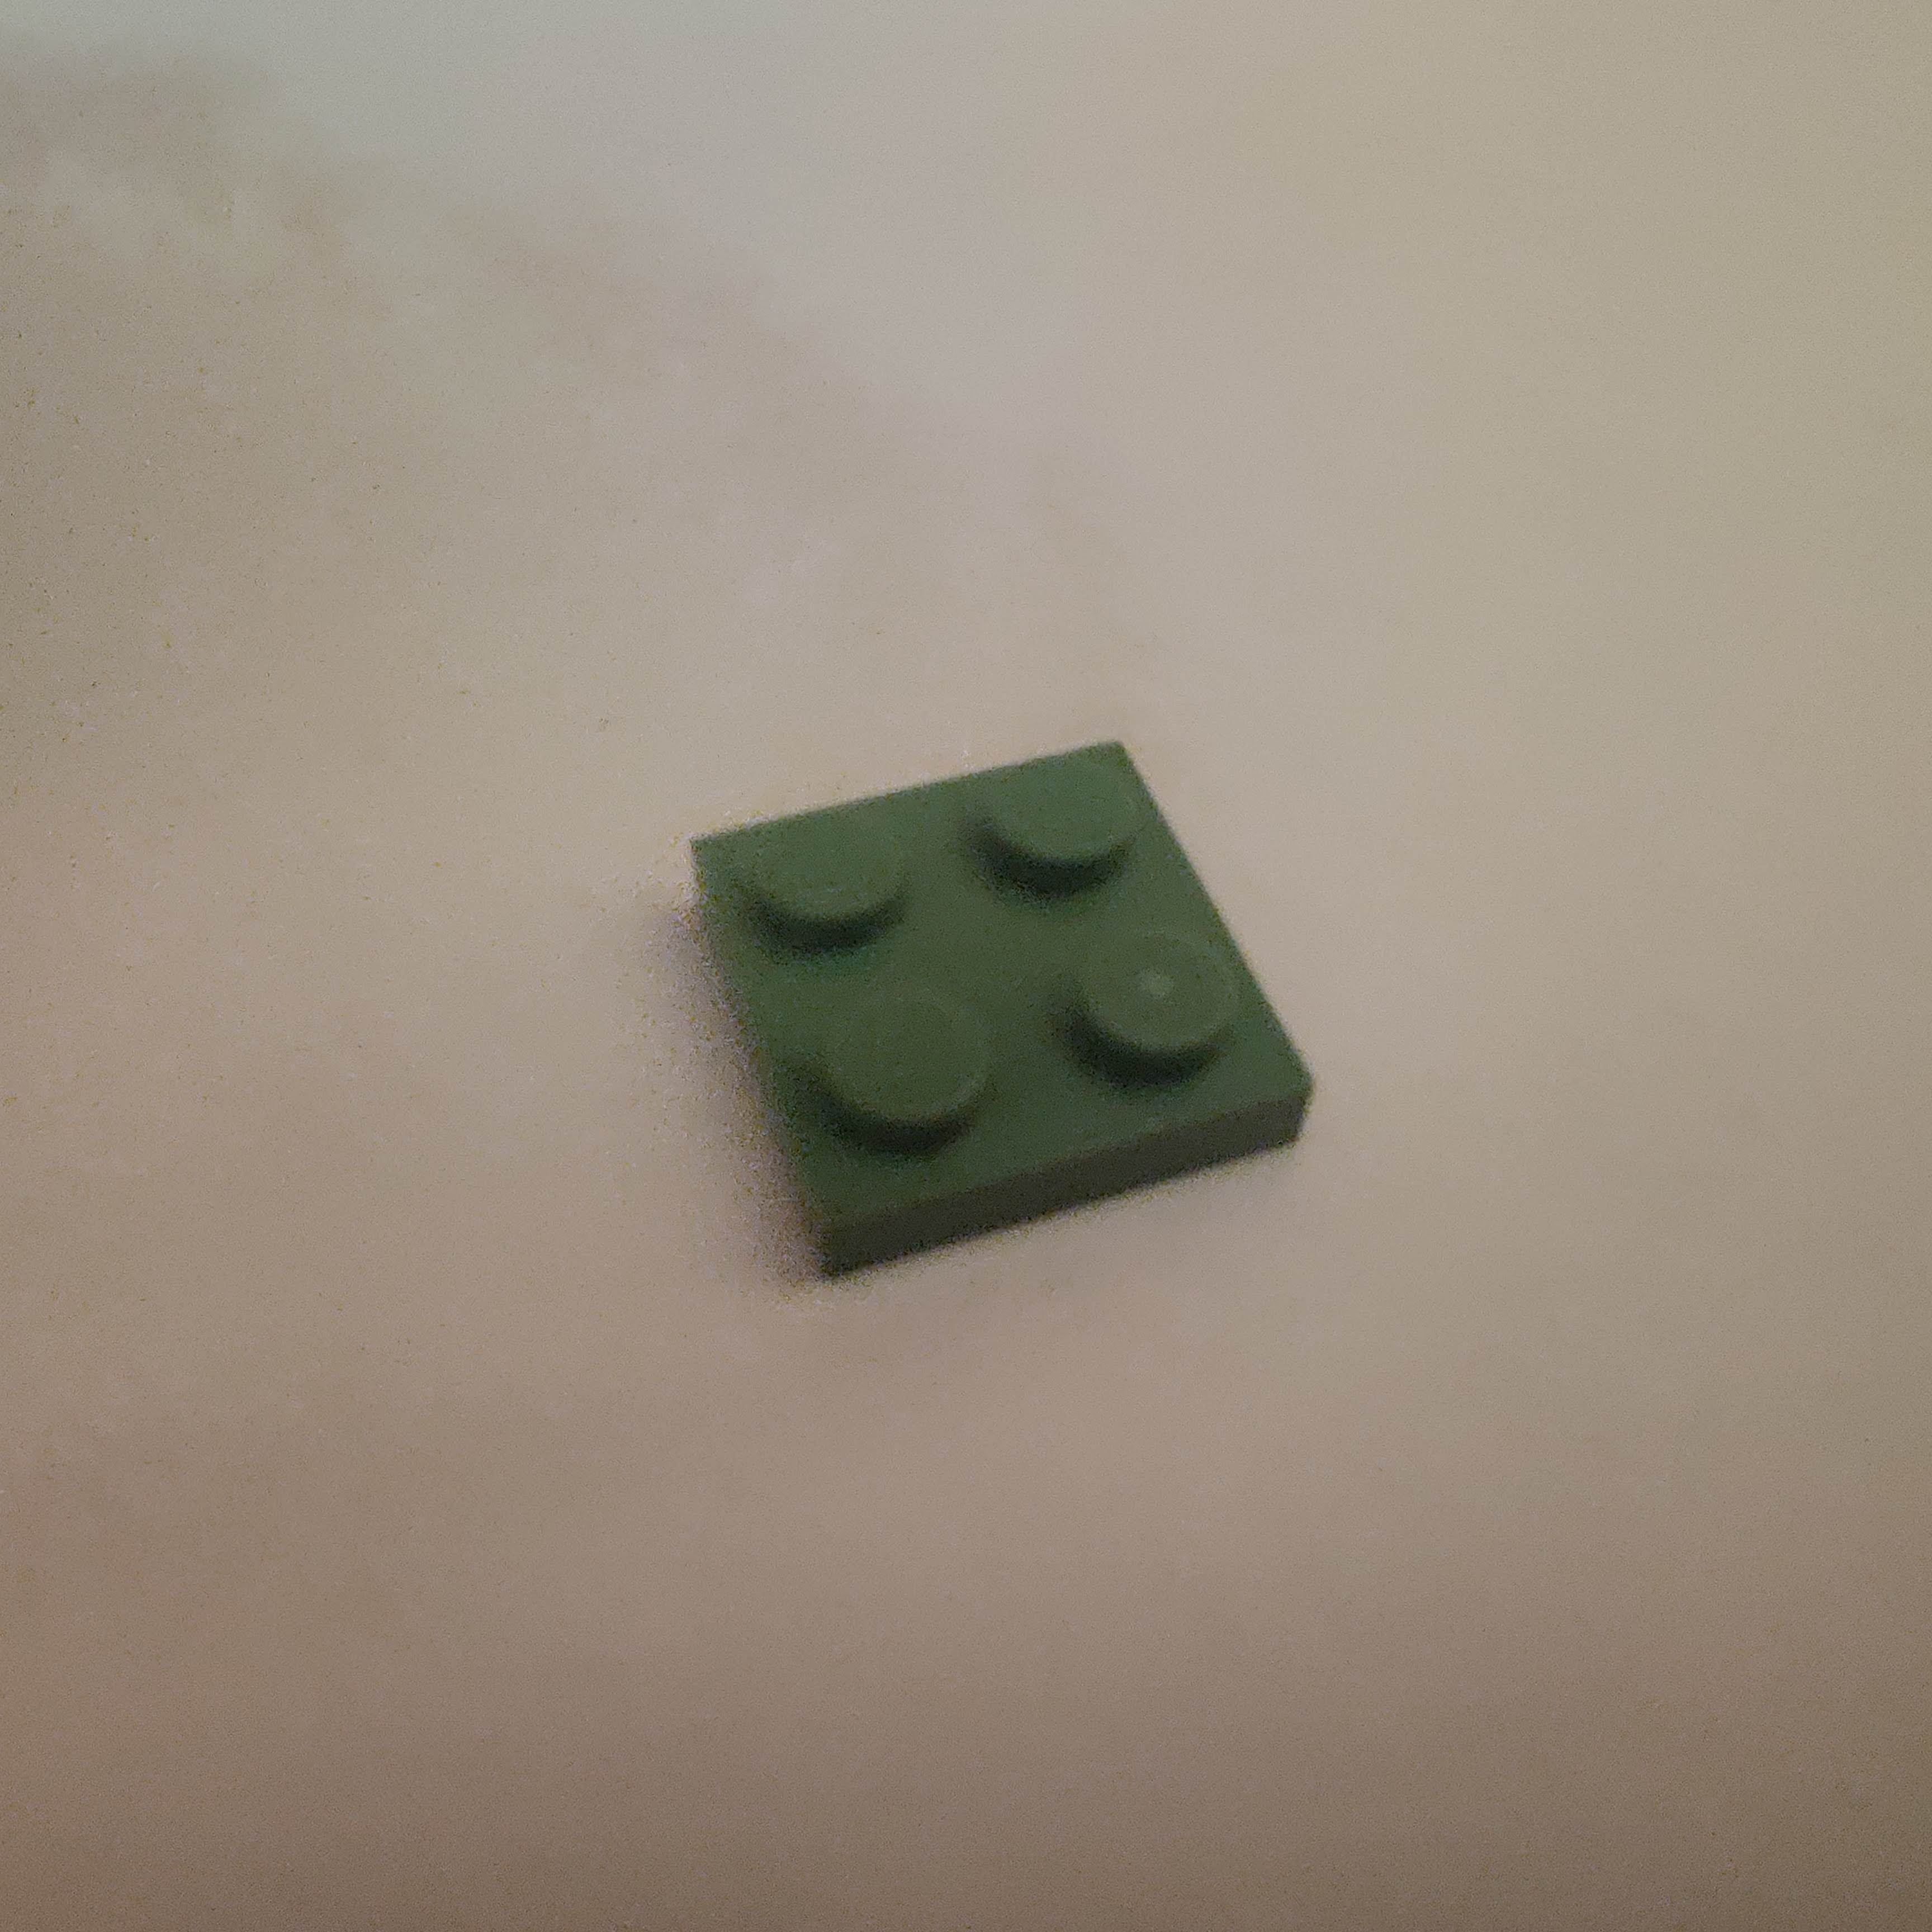
\includegraphics[width=\textwidth]{photographed images/11.jpg}
    \end{subfigure}
    \begin{subfigure}[b]{0.2\textwidth}
        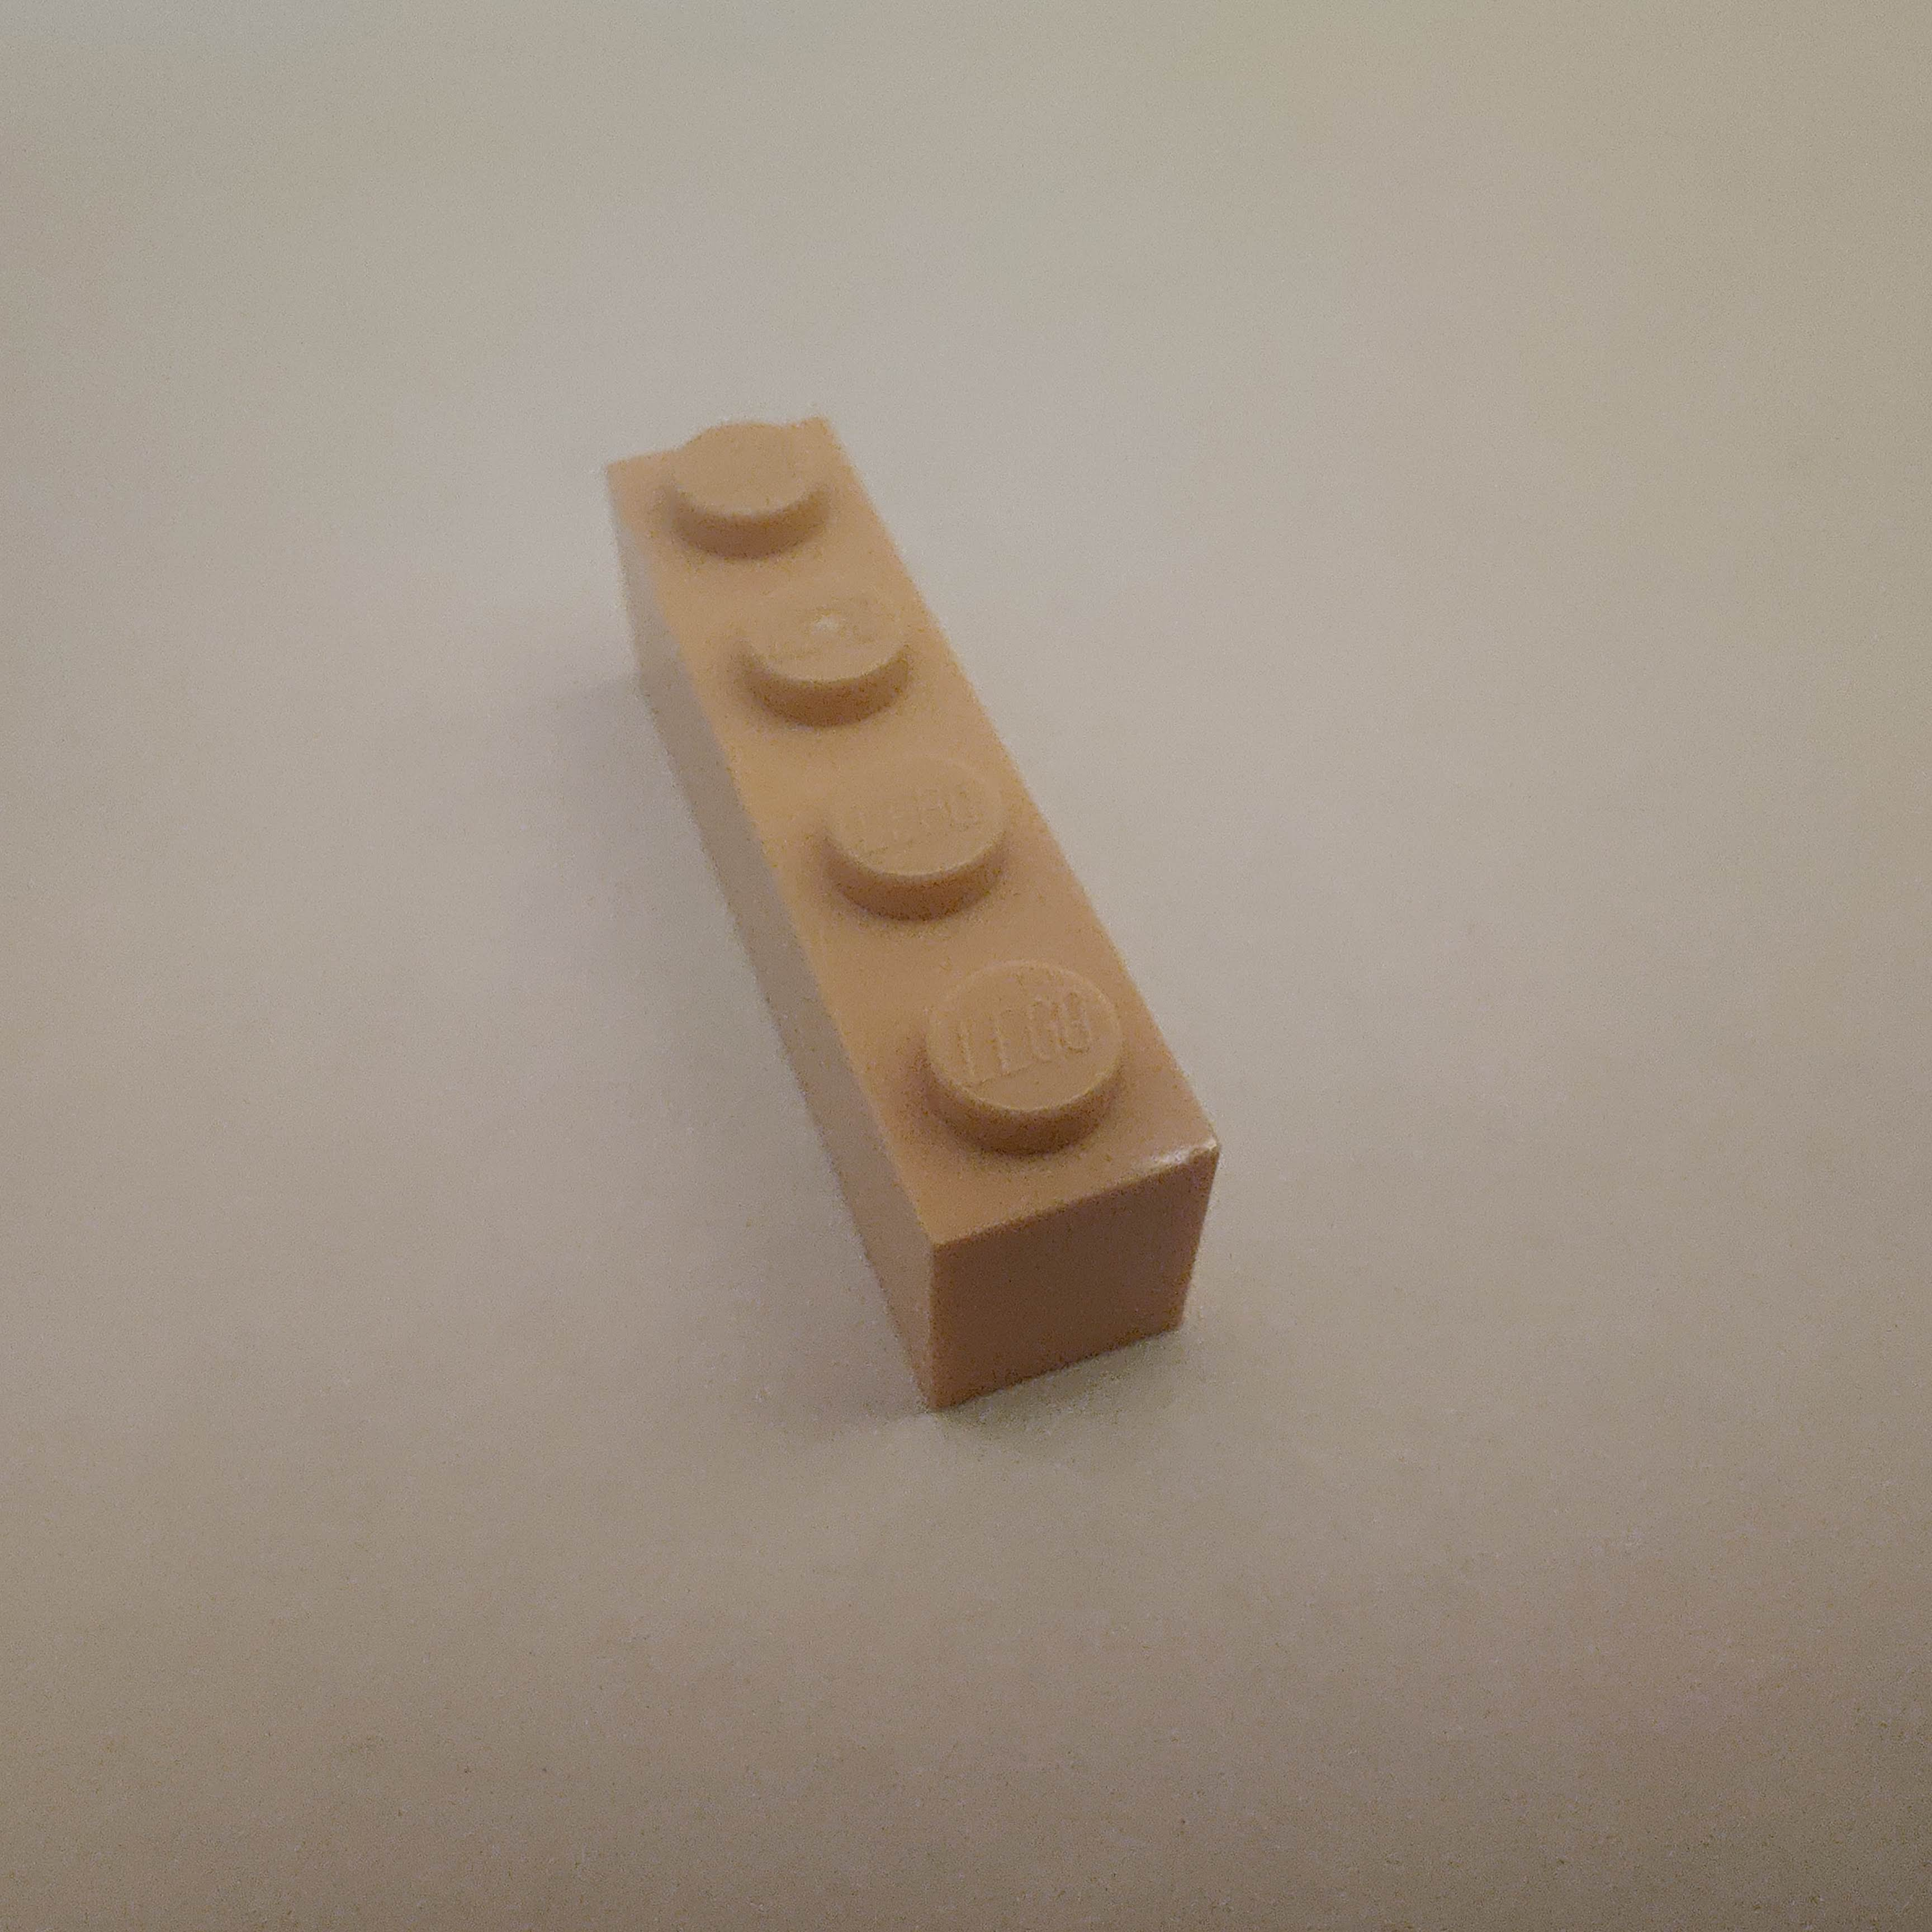
\includegraphics[width=\textwidth]{photographed images/12.jpg}
    \end{subfigure}
    \begin{subfigure}[b]{0.2\textwidth}
        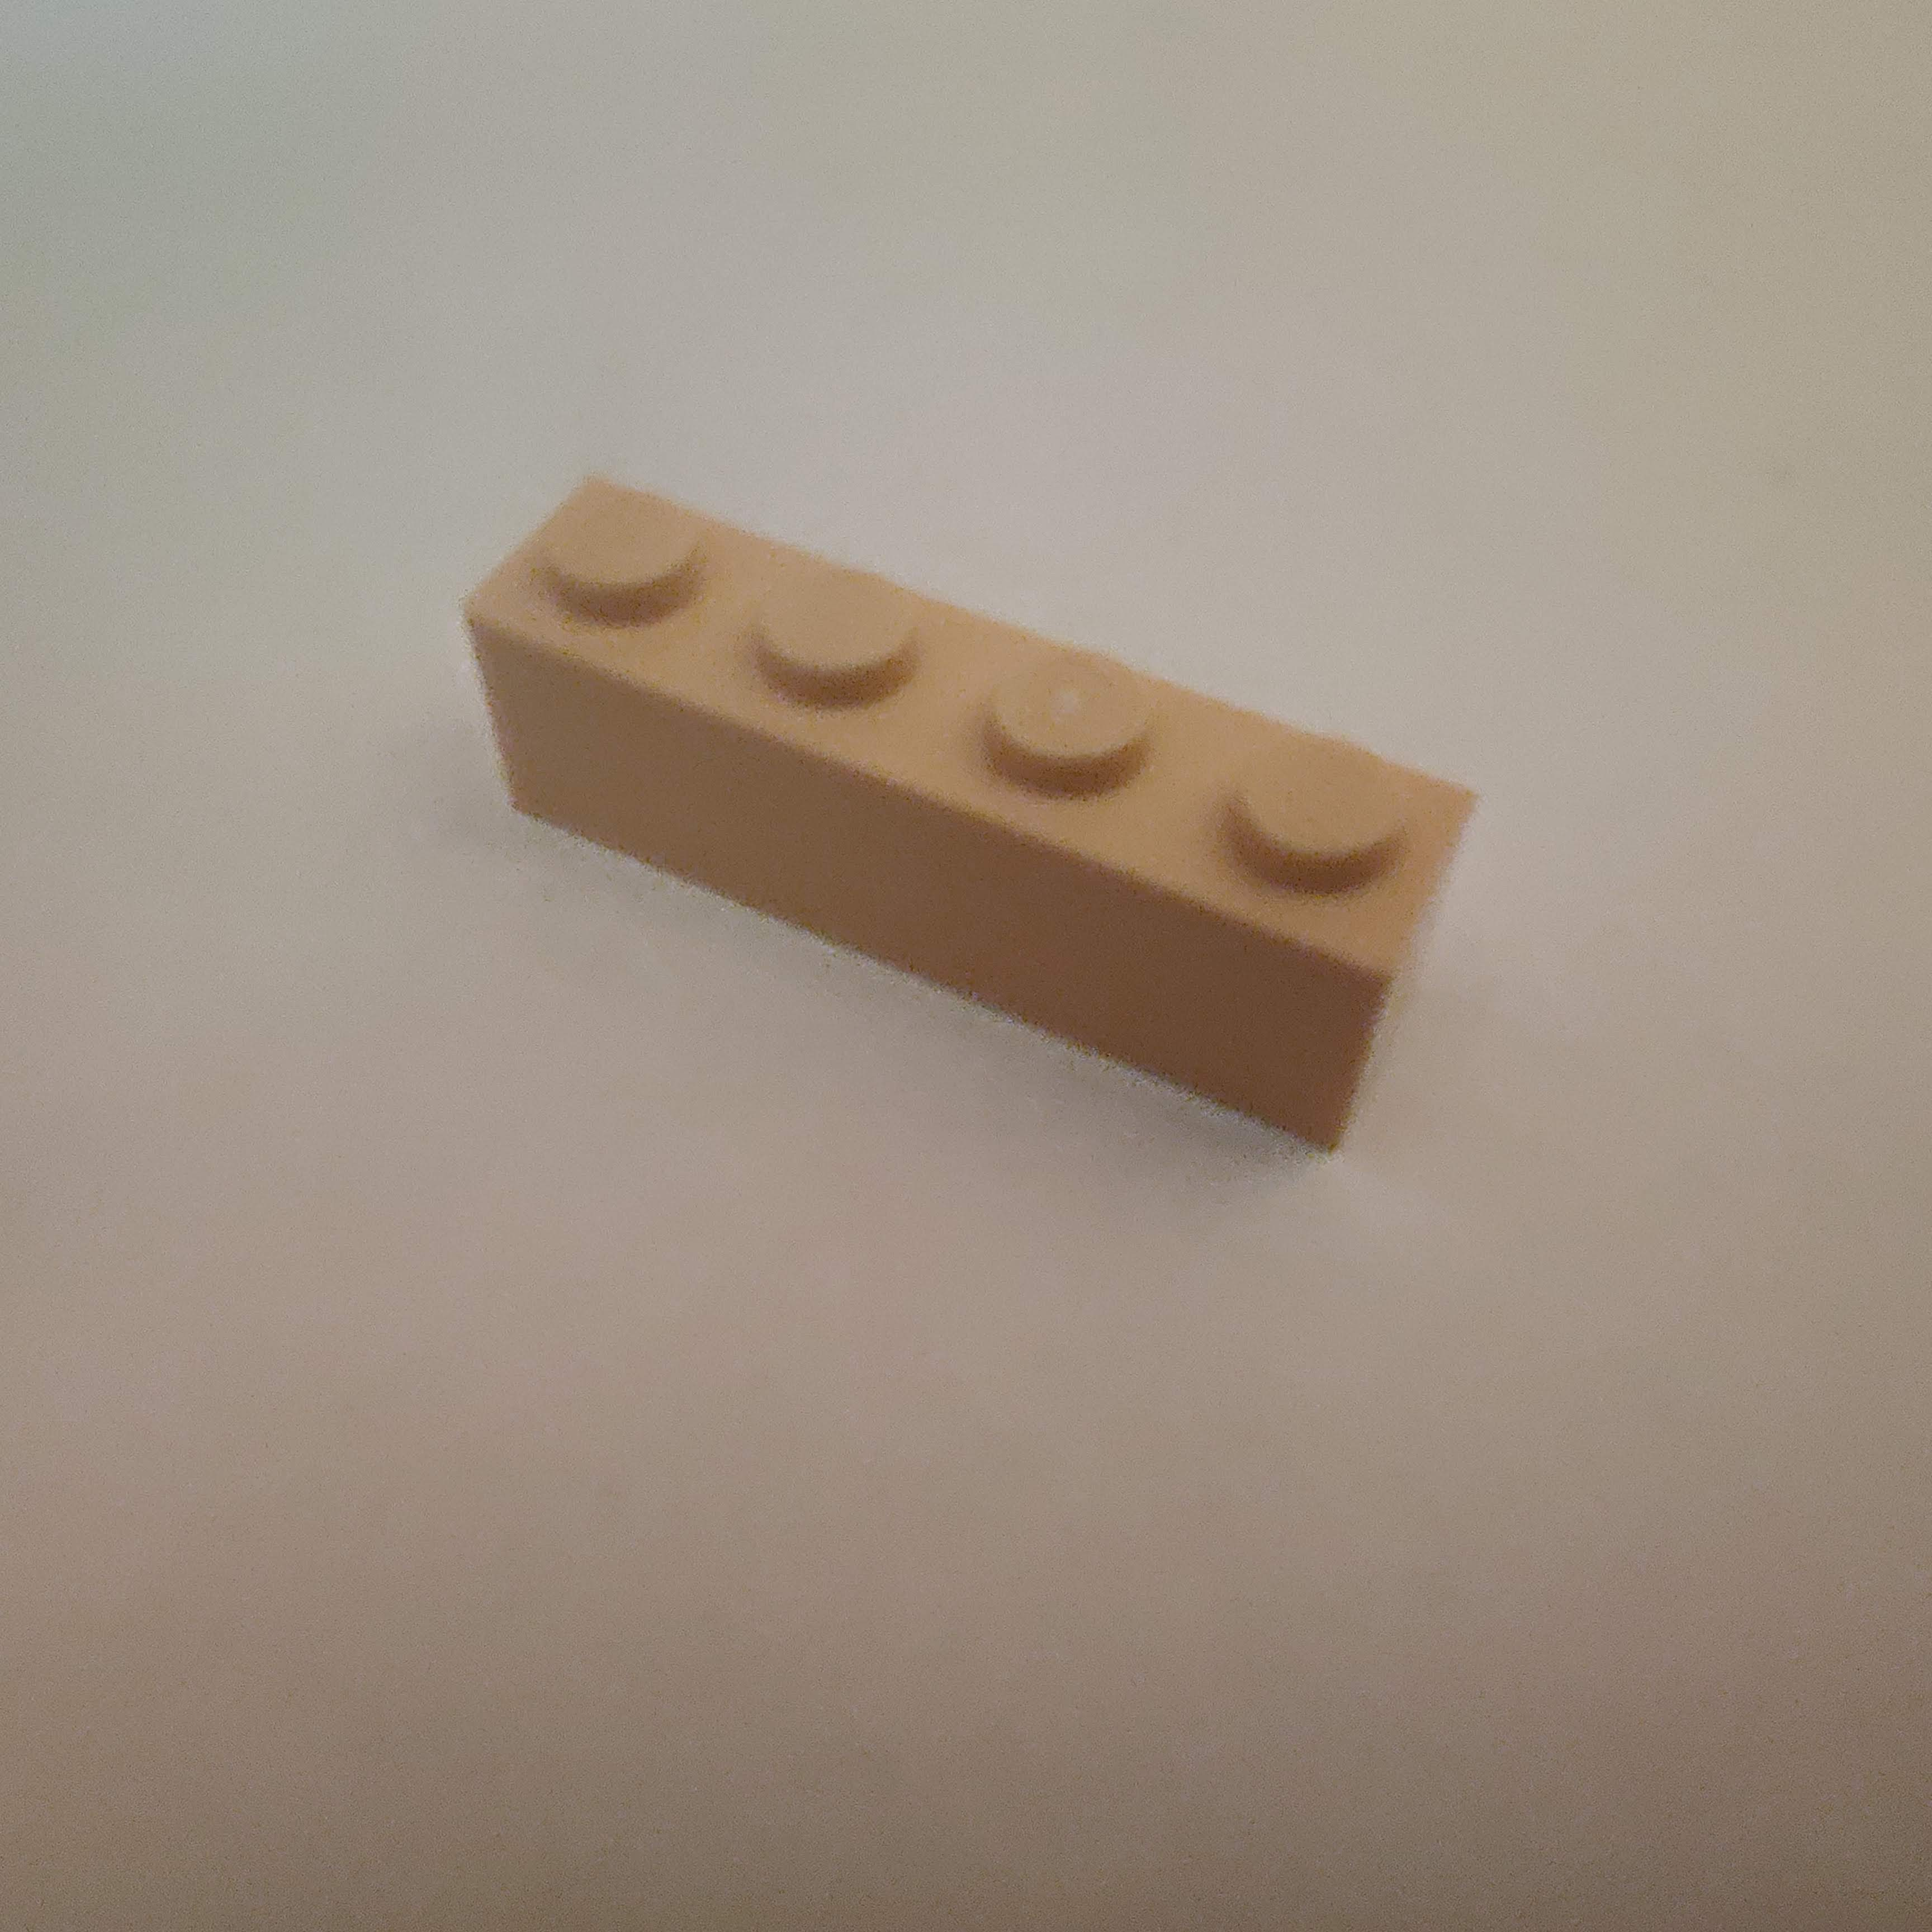
\includegraphics[width=\textwidth]{photographed images/13.jpg}
    \end{subfigure}
    \begin{subfigure}[b]{0.2\textwidth}
        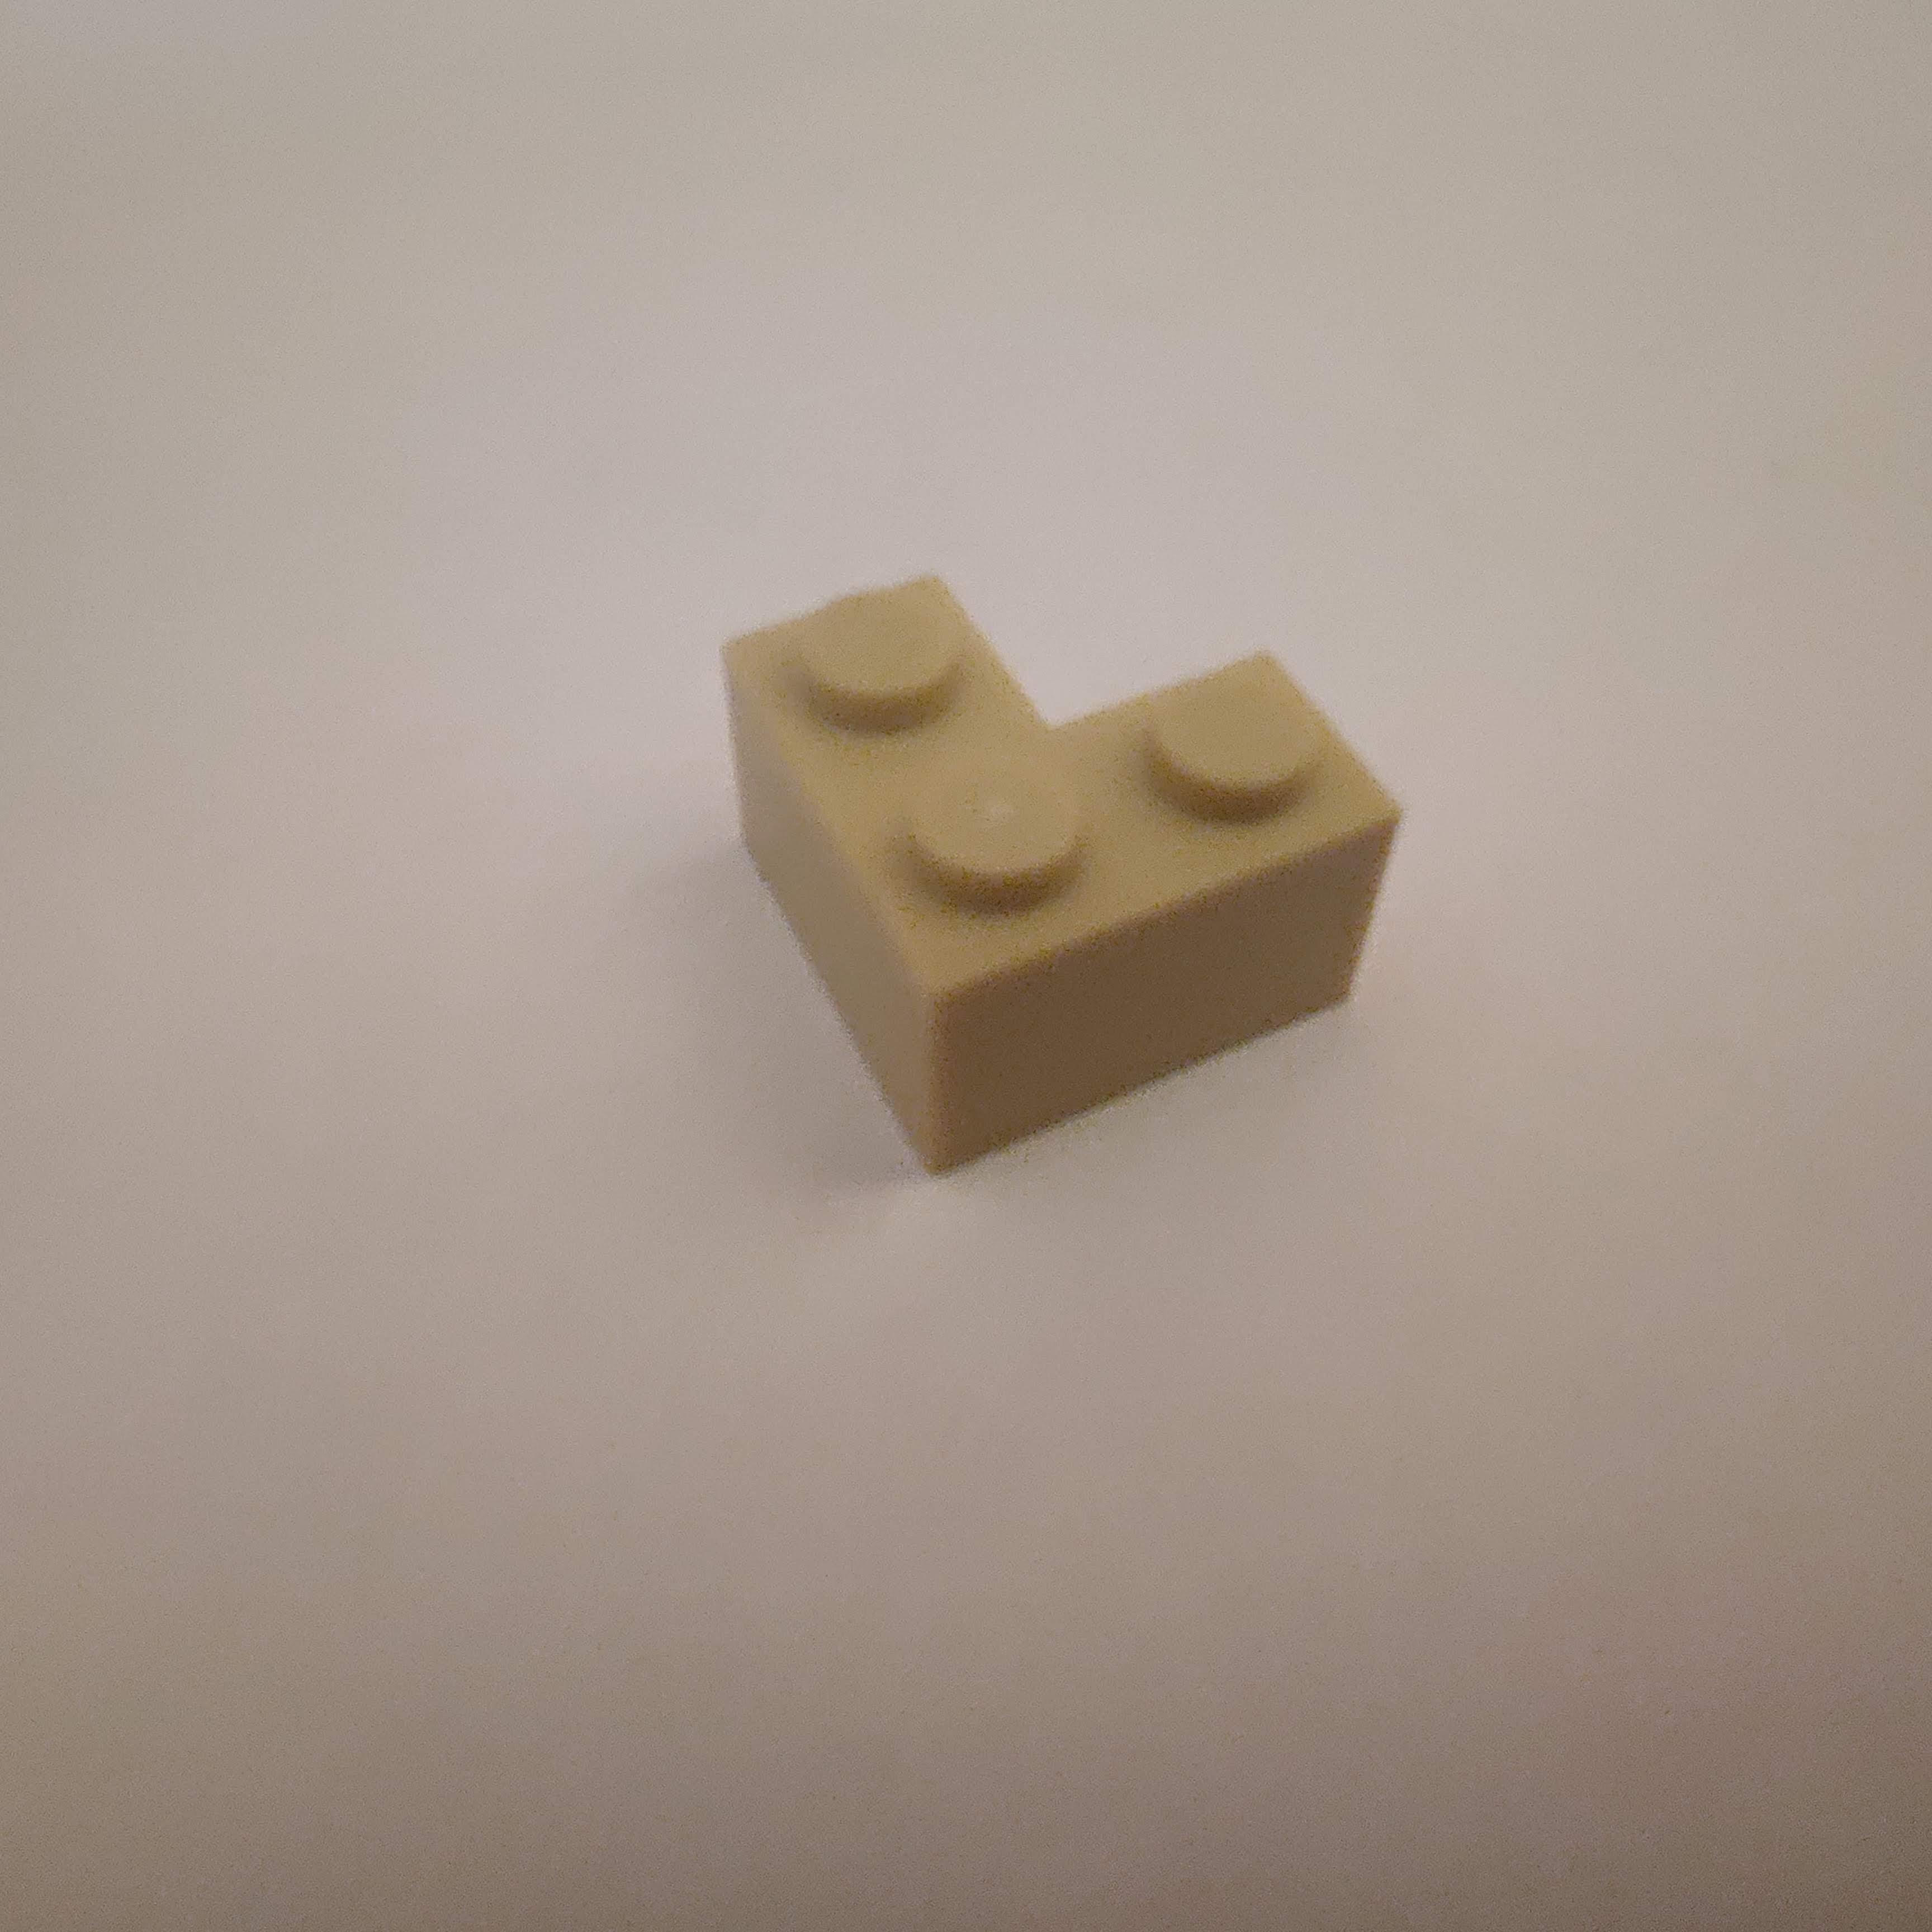
\includegraphics[width=\textwidth]{photographed images/14.jpg}
    \end{subfigure}
    \begin{subfigure}[b]{0.2\textwidth}
        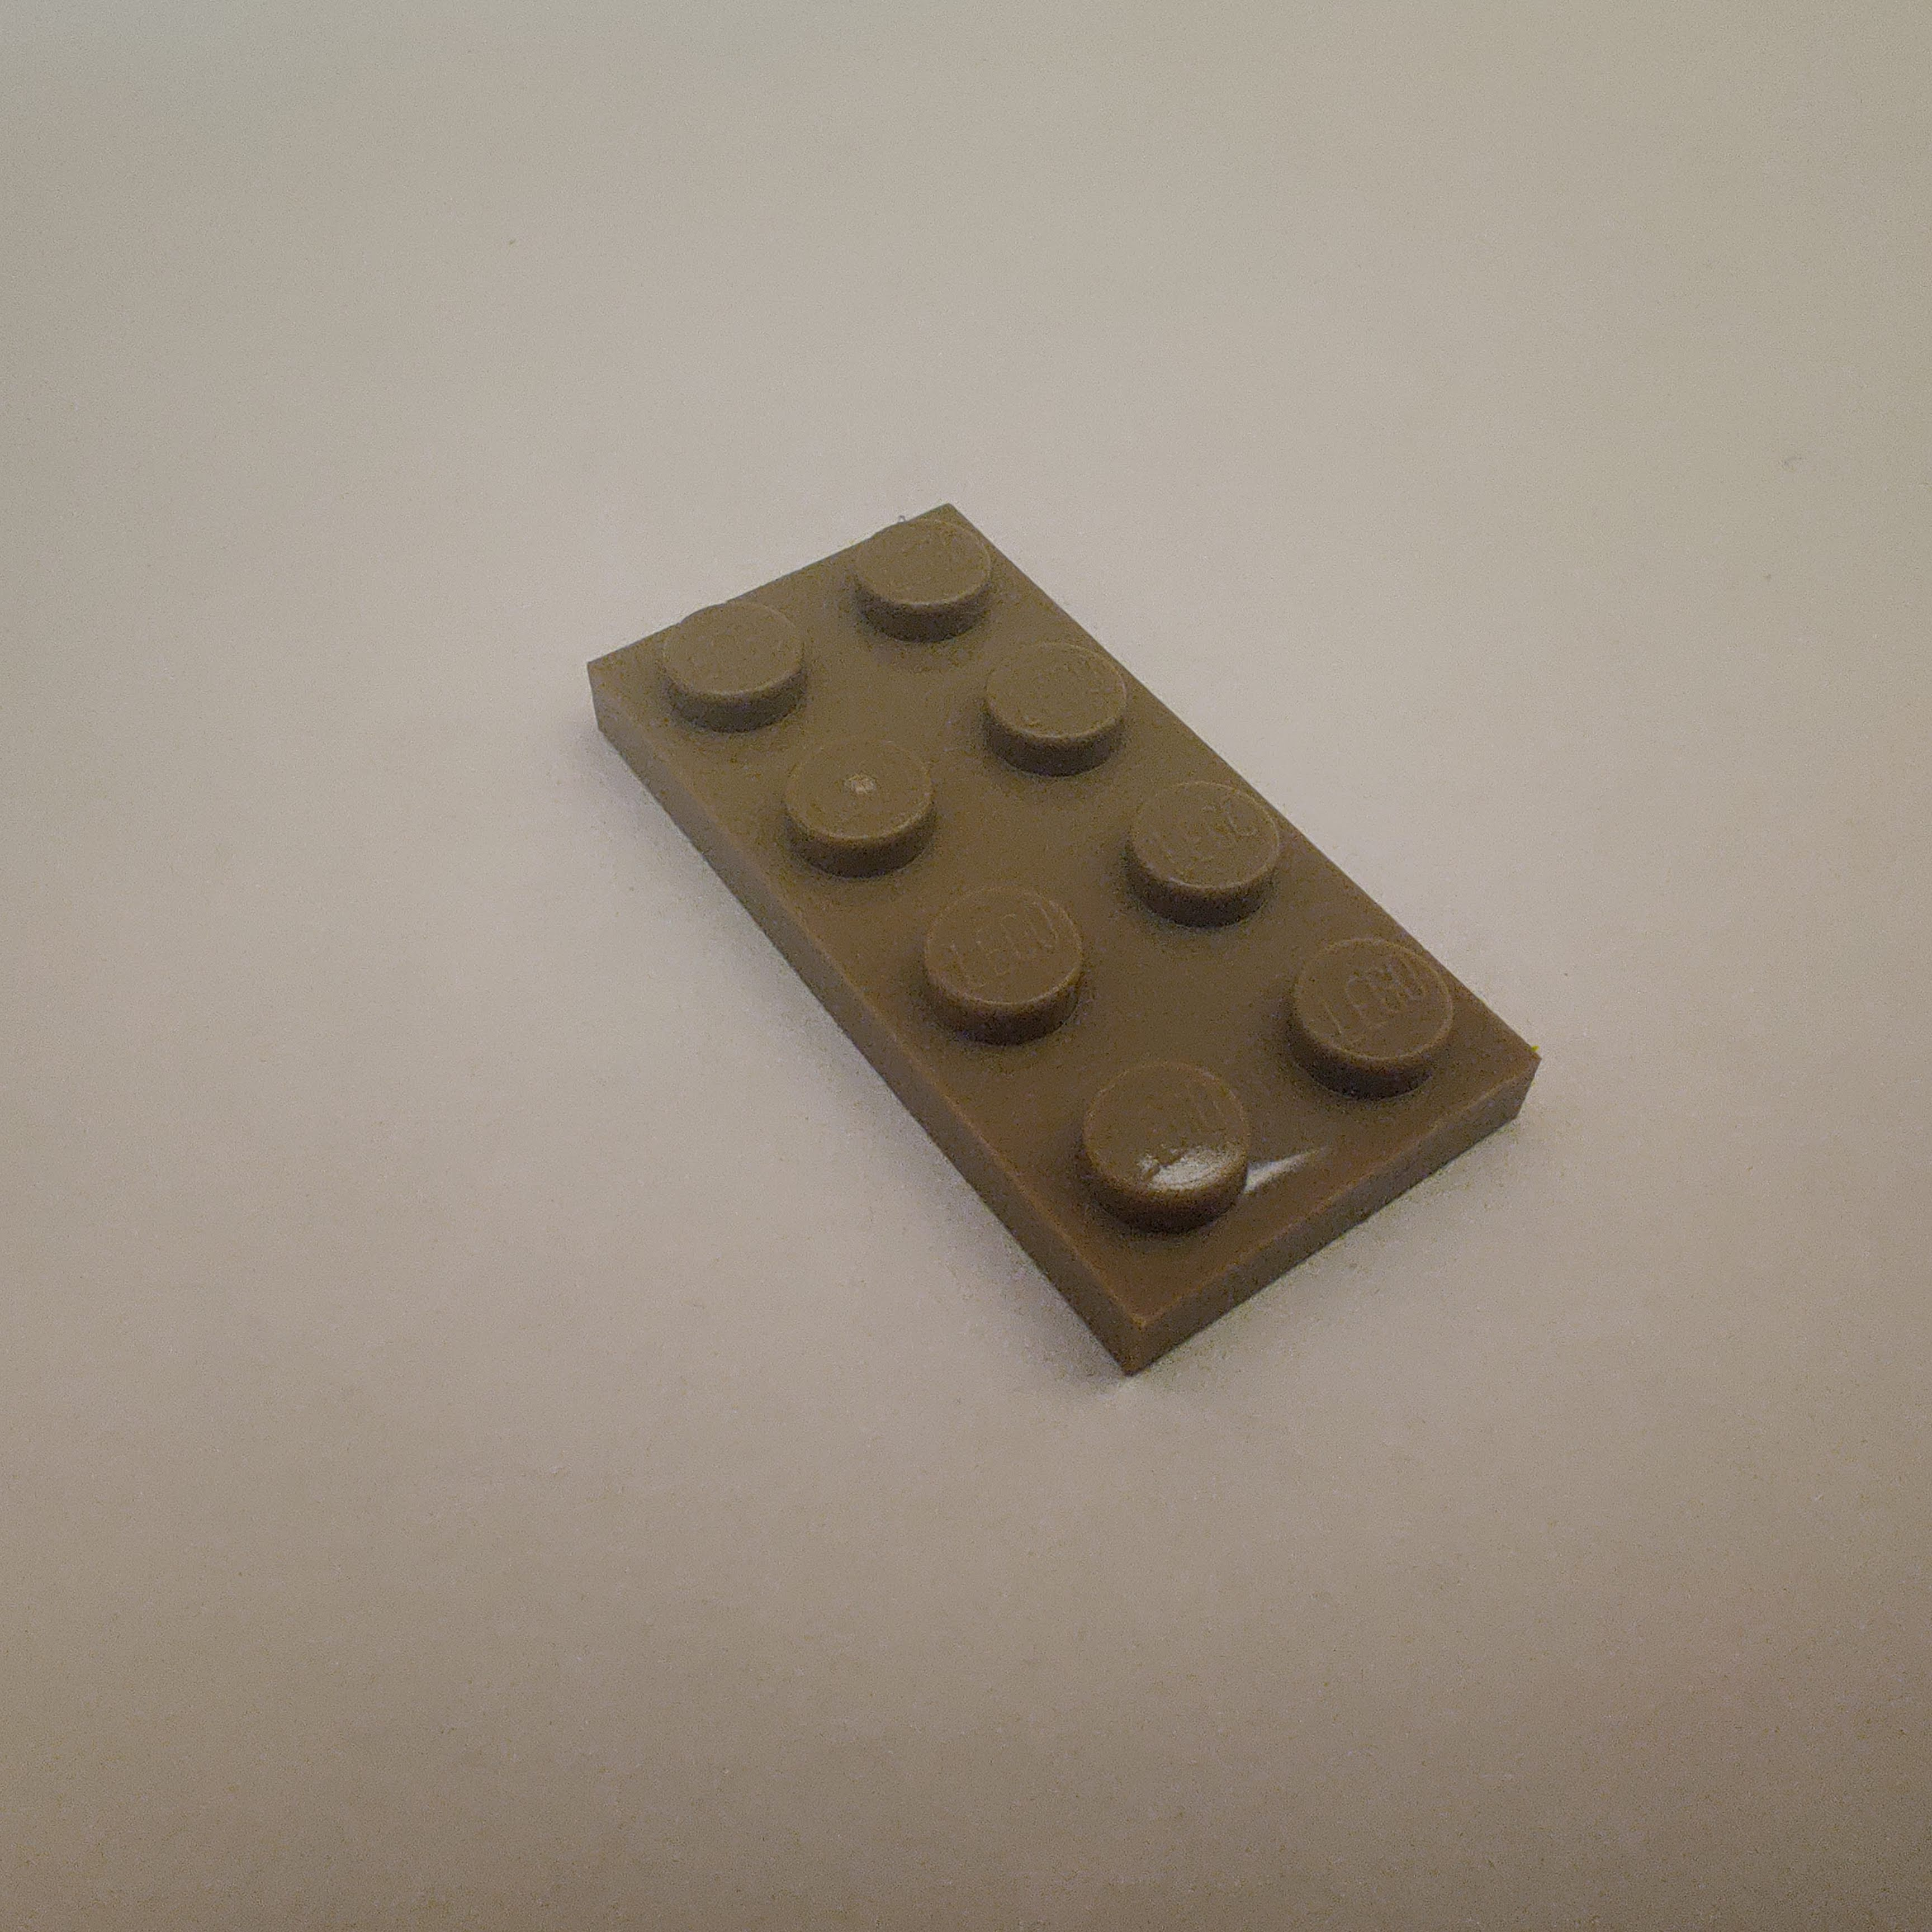
\includegraphics[width=\textwidth]{photographed images/15.jpg}
    \end{subfigure}
    \begin{subfigure}[b]{0.2\textwidth}
        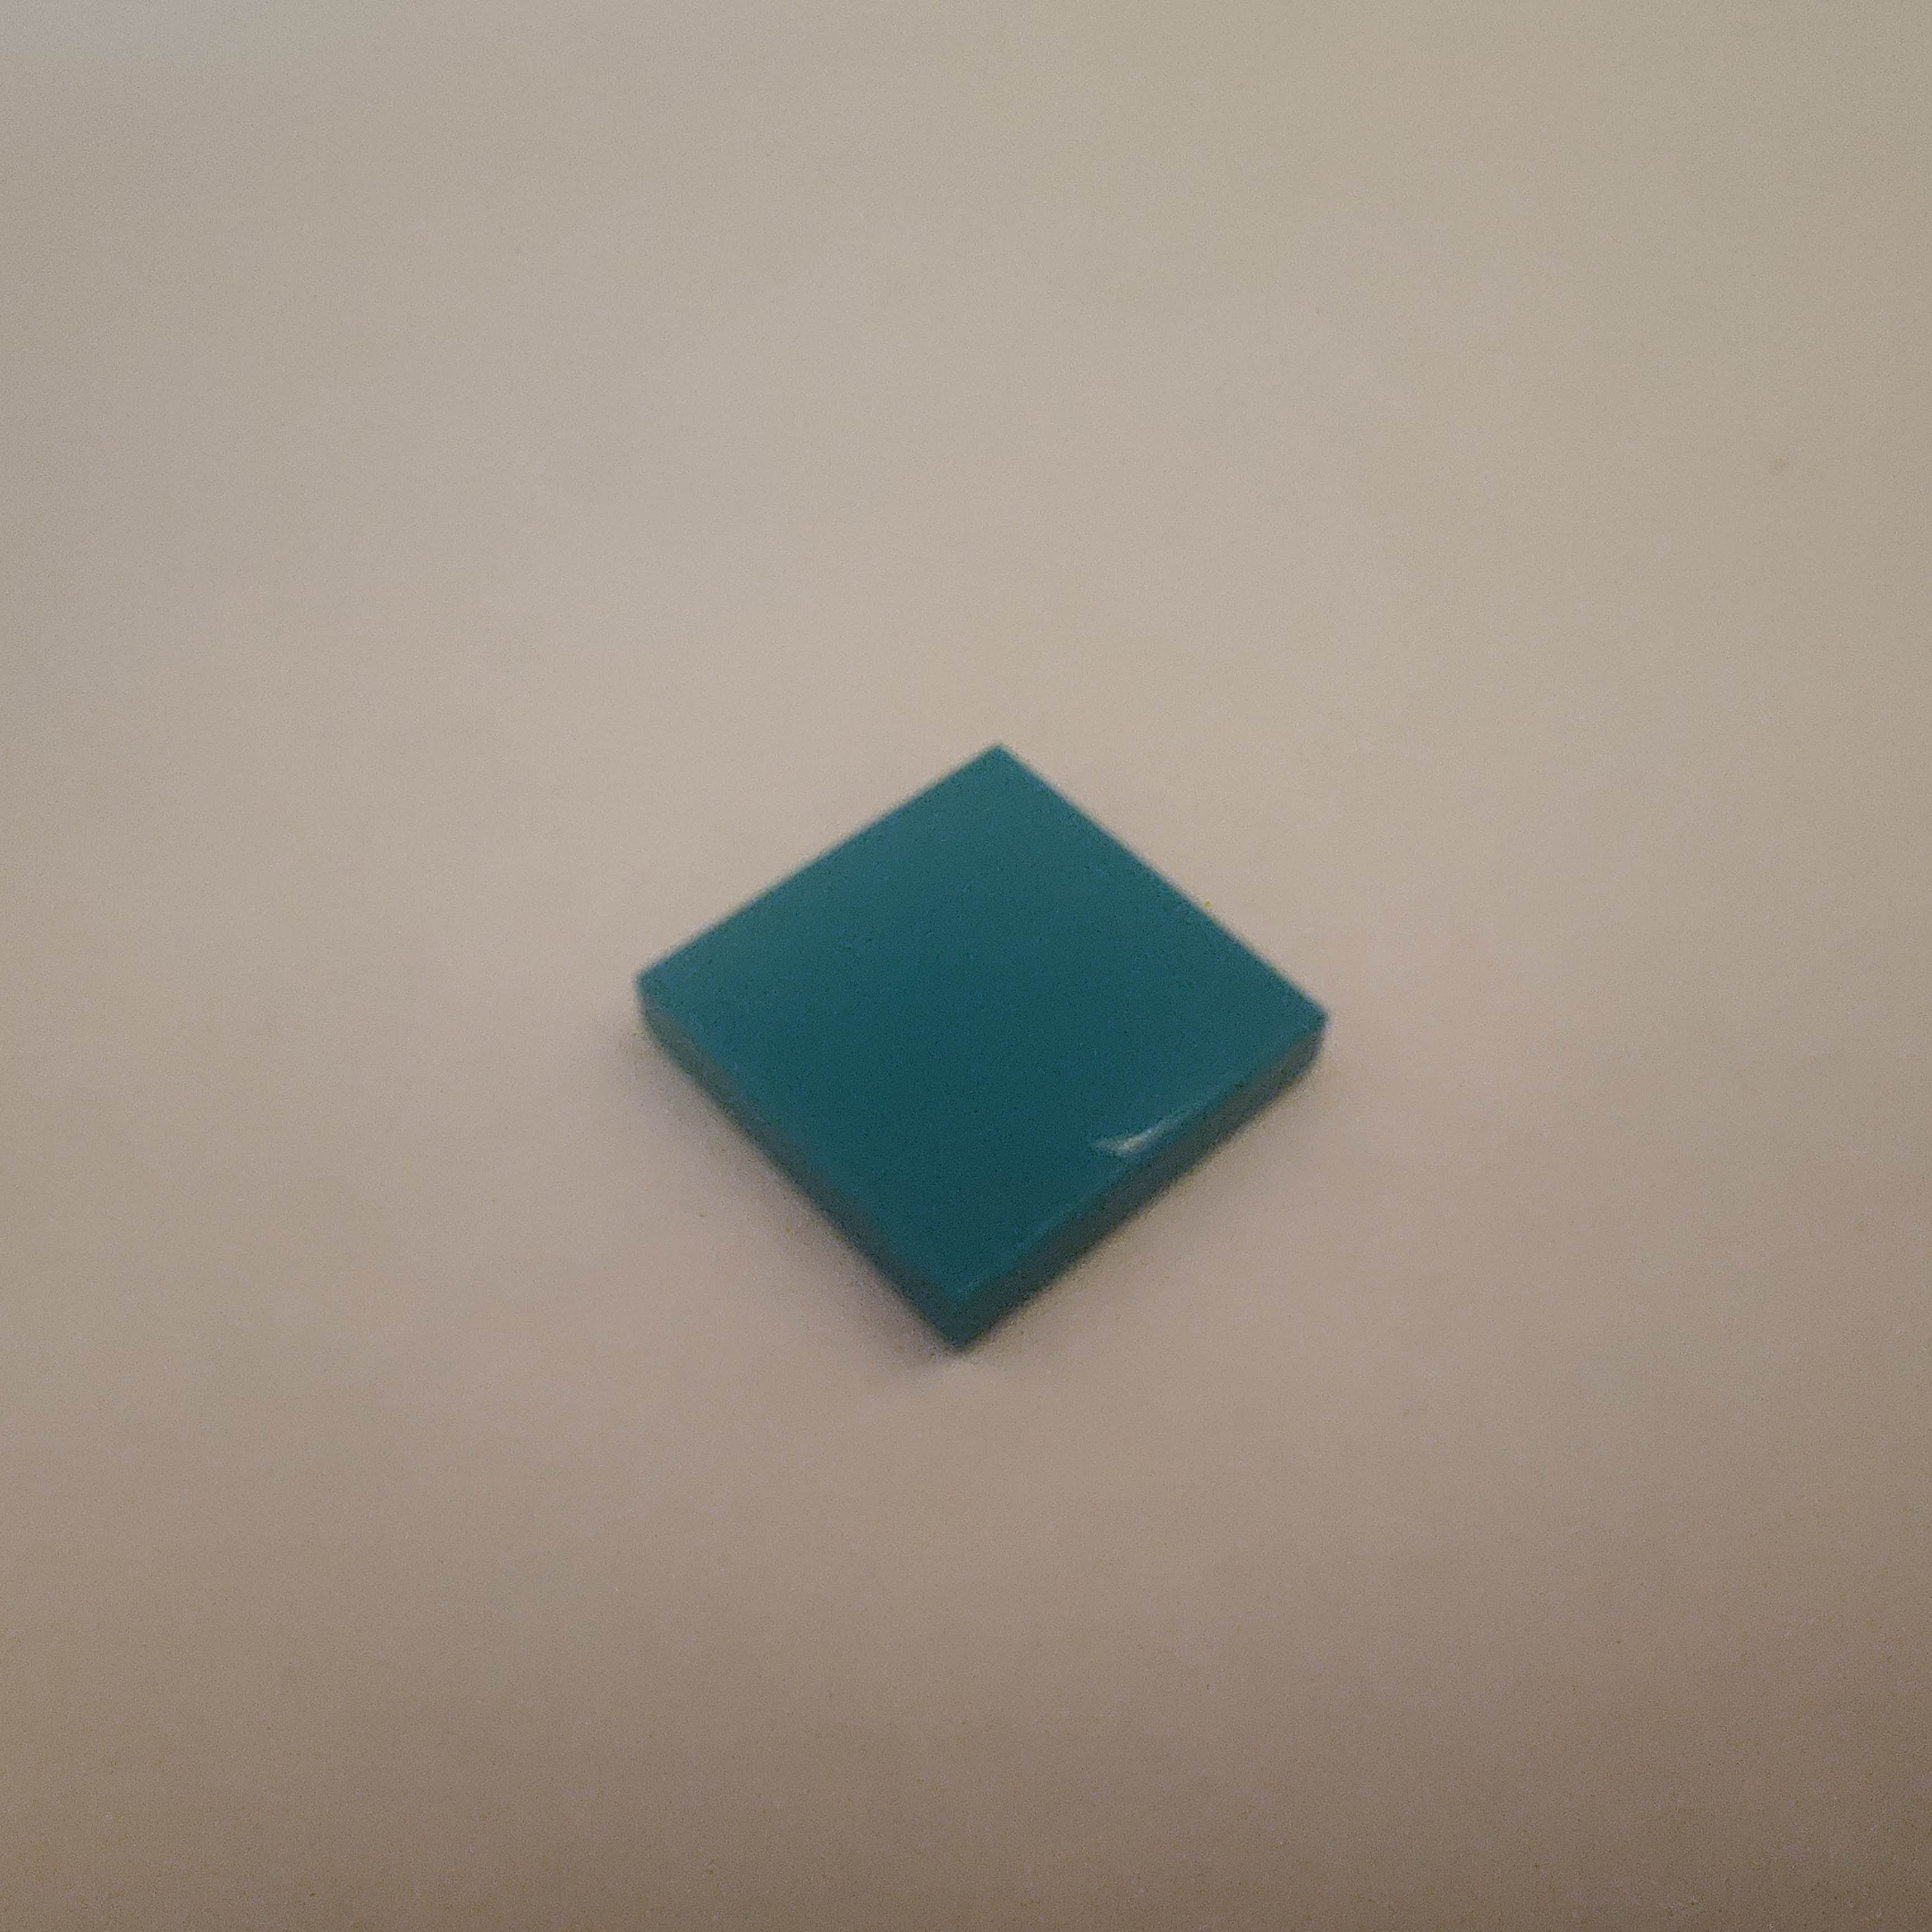
\includegraphics[width=\textwidth]{photographed images/16.jpg}
    \end{subfigure}
    \begin{subfigure}[b]{0.2\textwidth}
        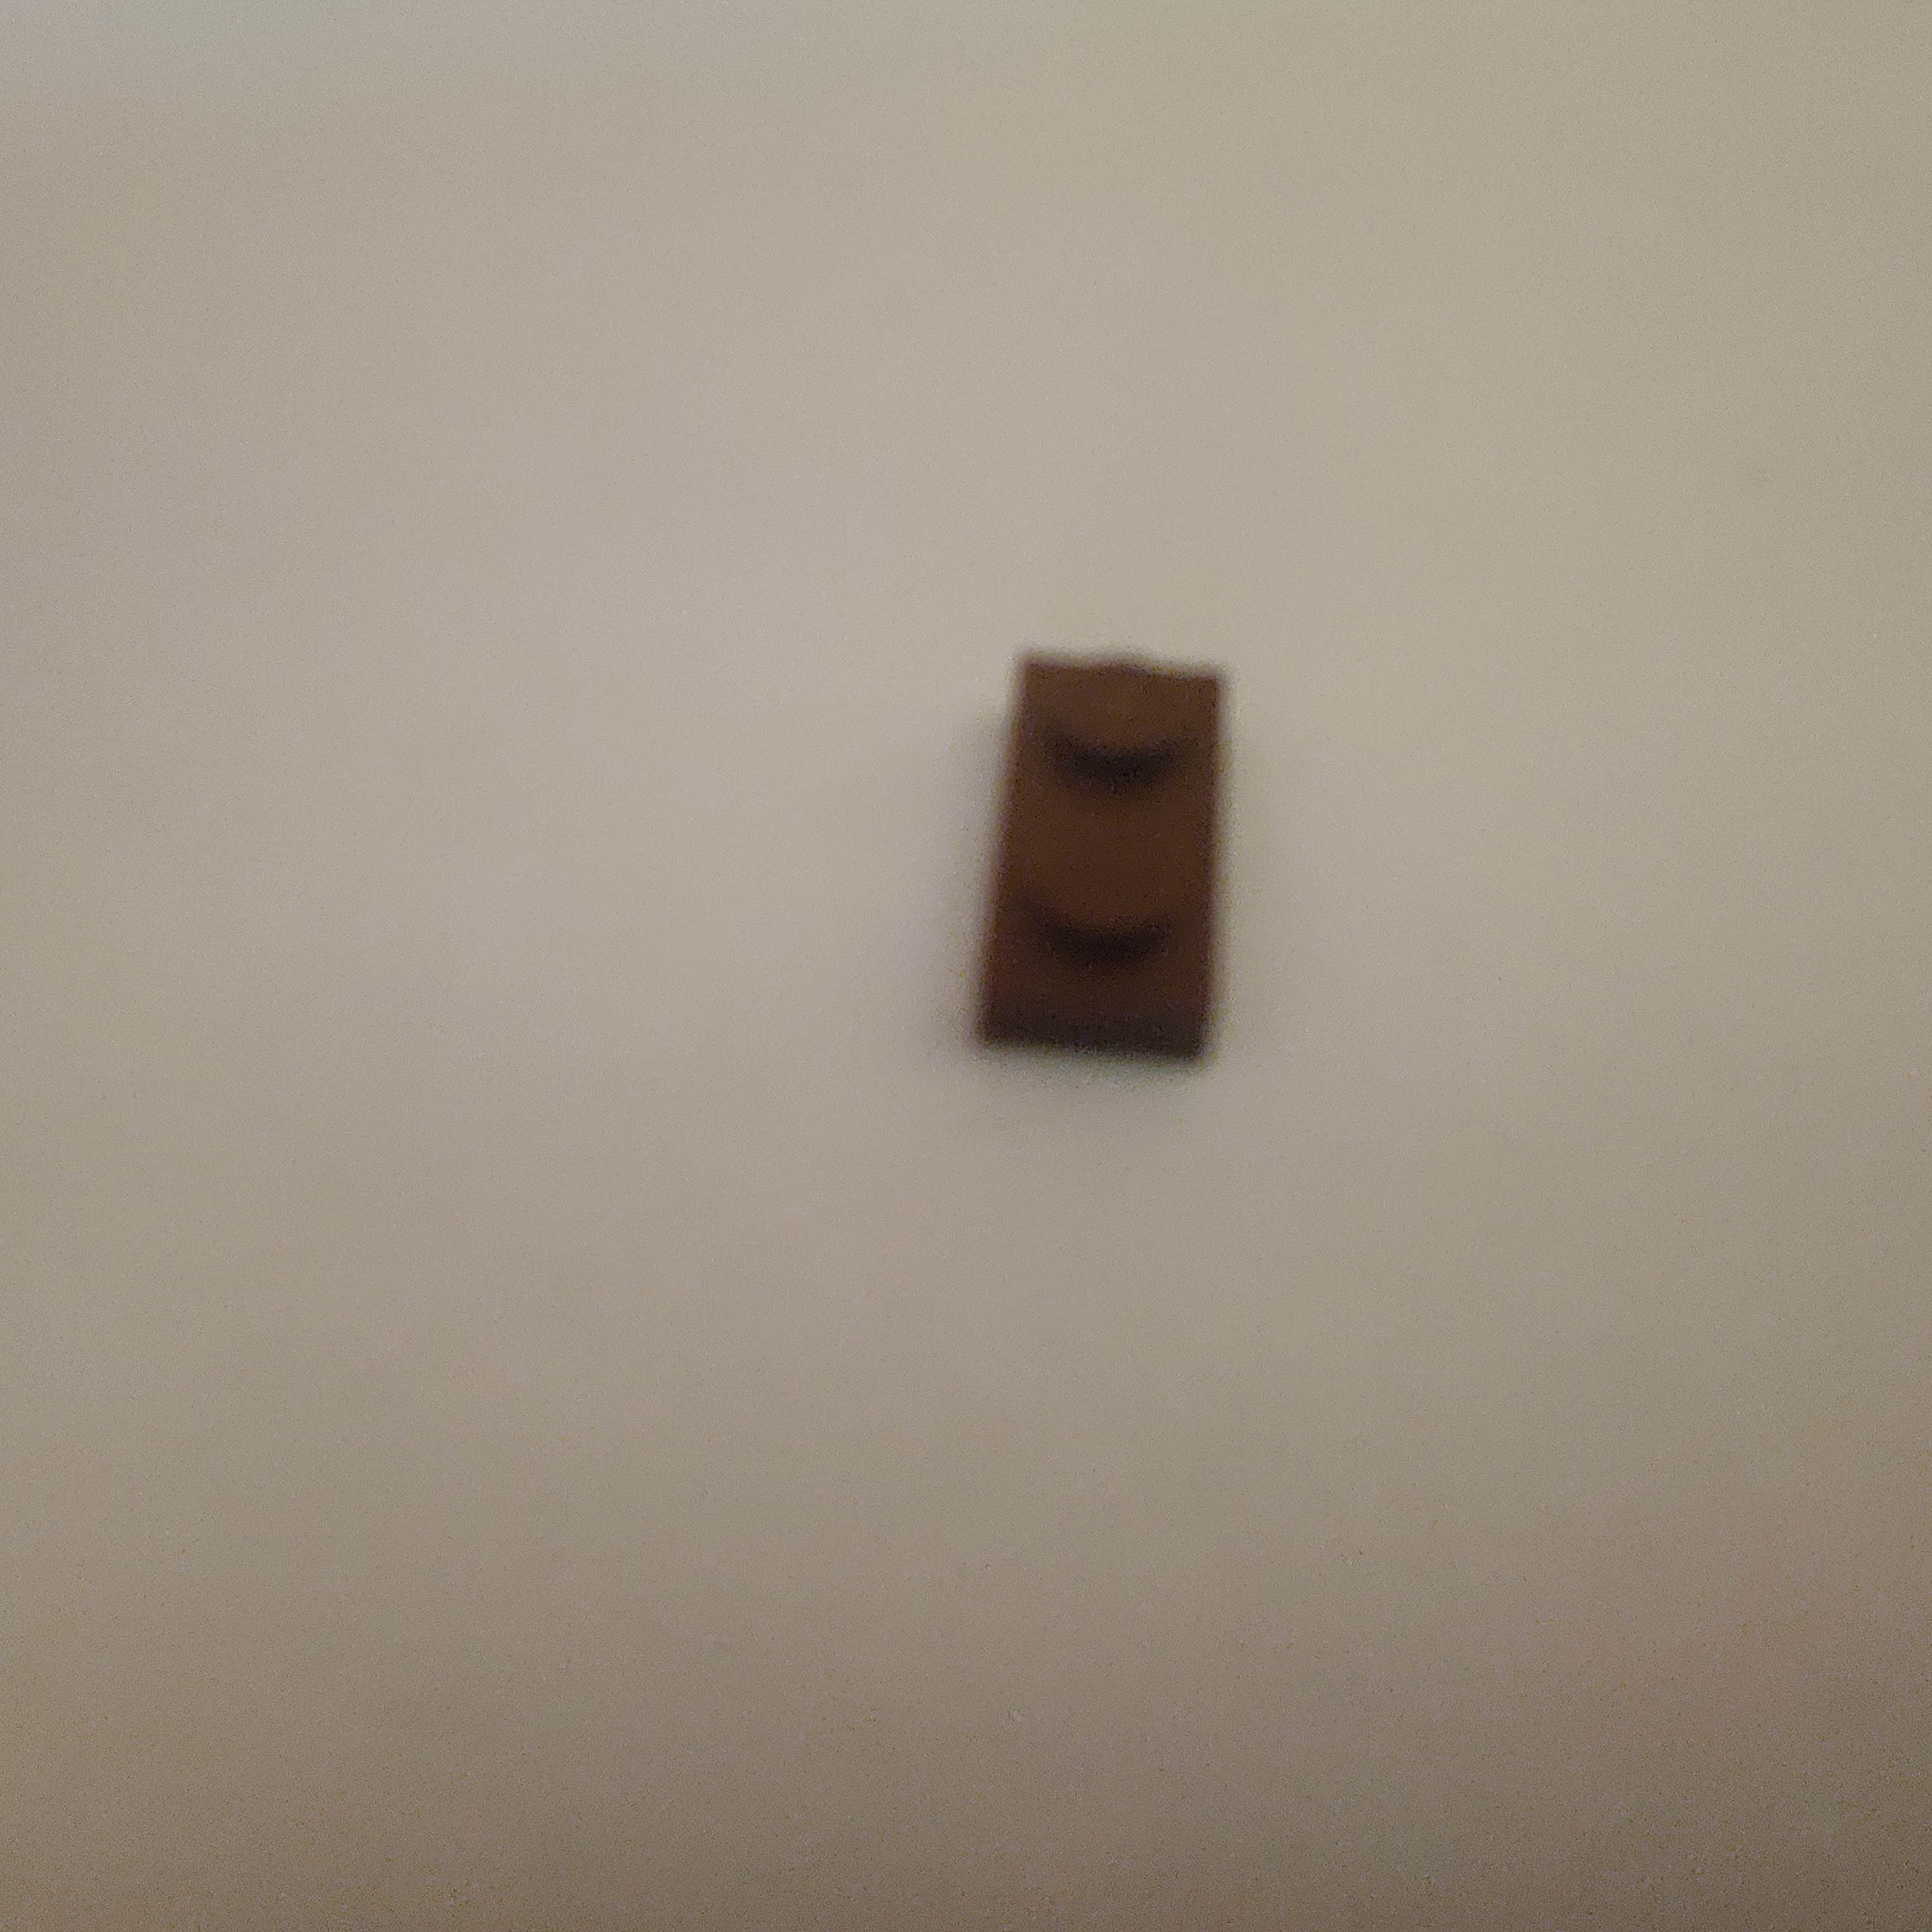
\includegraphics[width=\textwidth]{photographed images/17.jpg}
    \end{subfigure}
    \begin{subfigure}[b]{0.2\textwidth}
        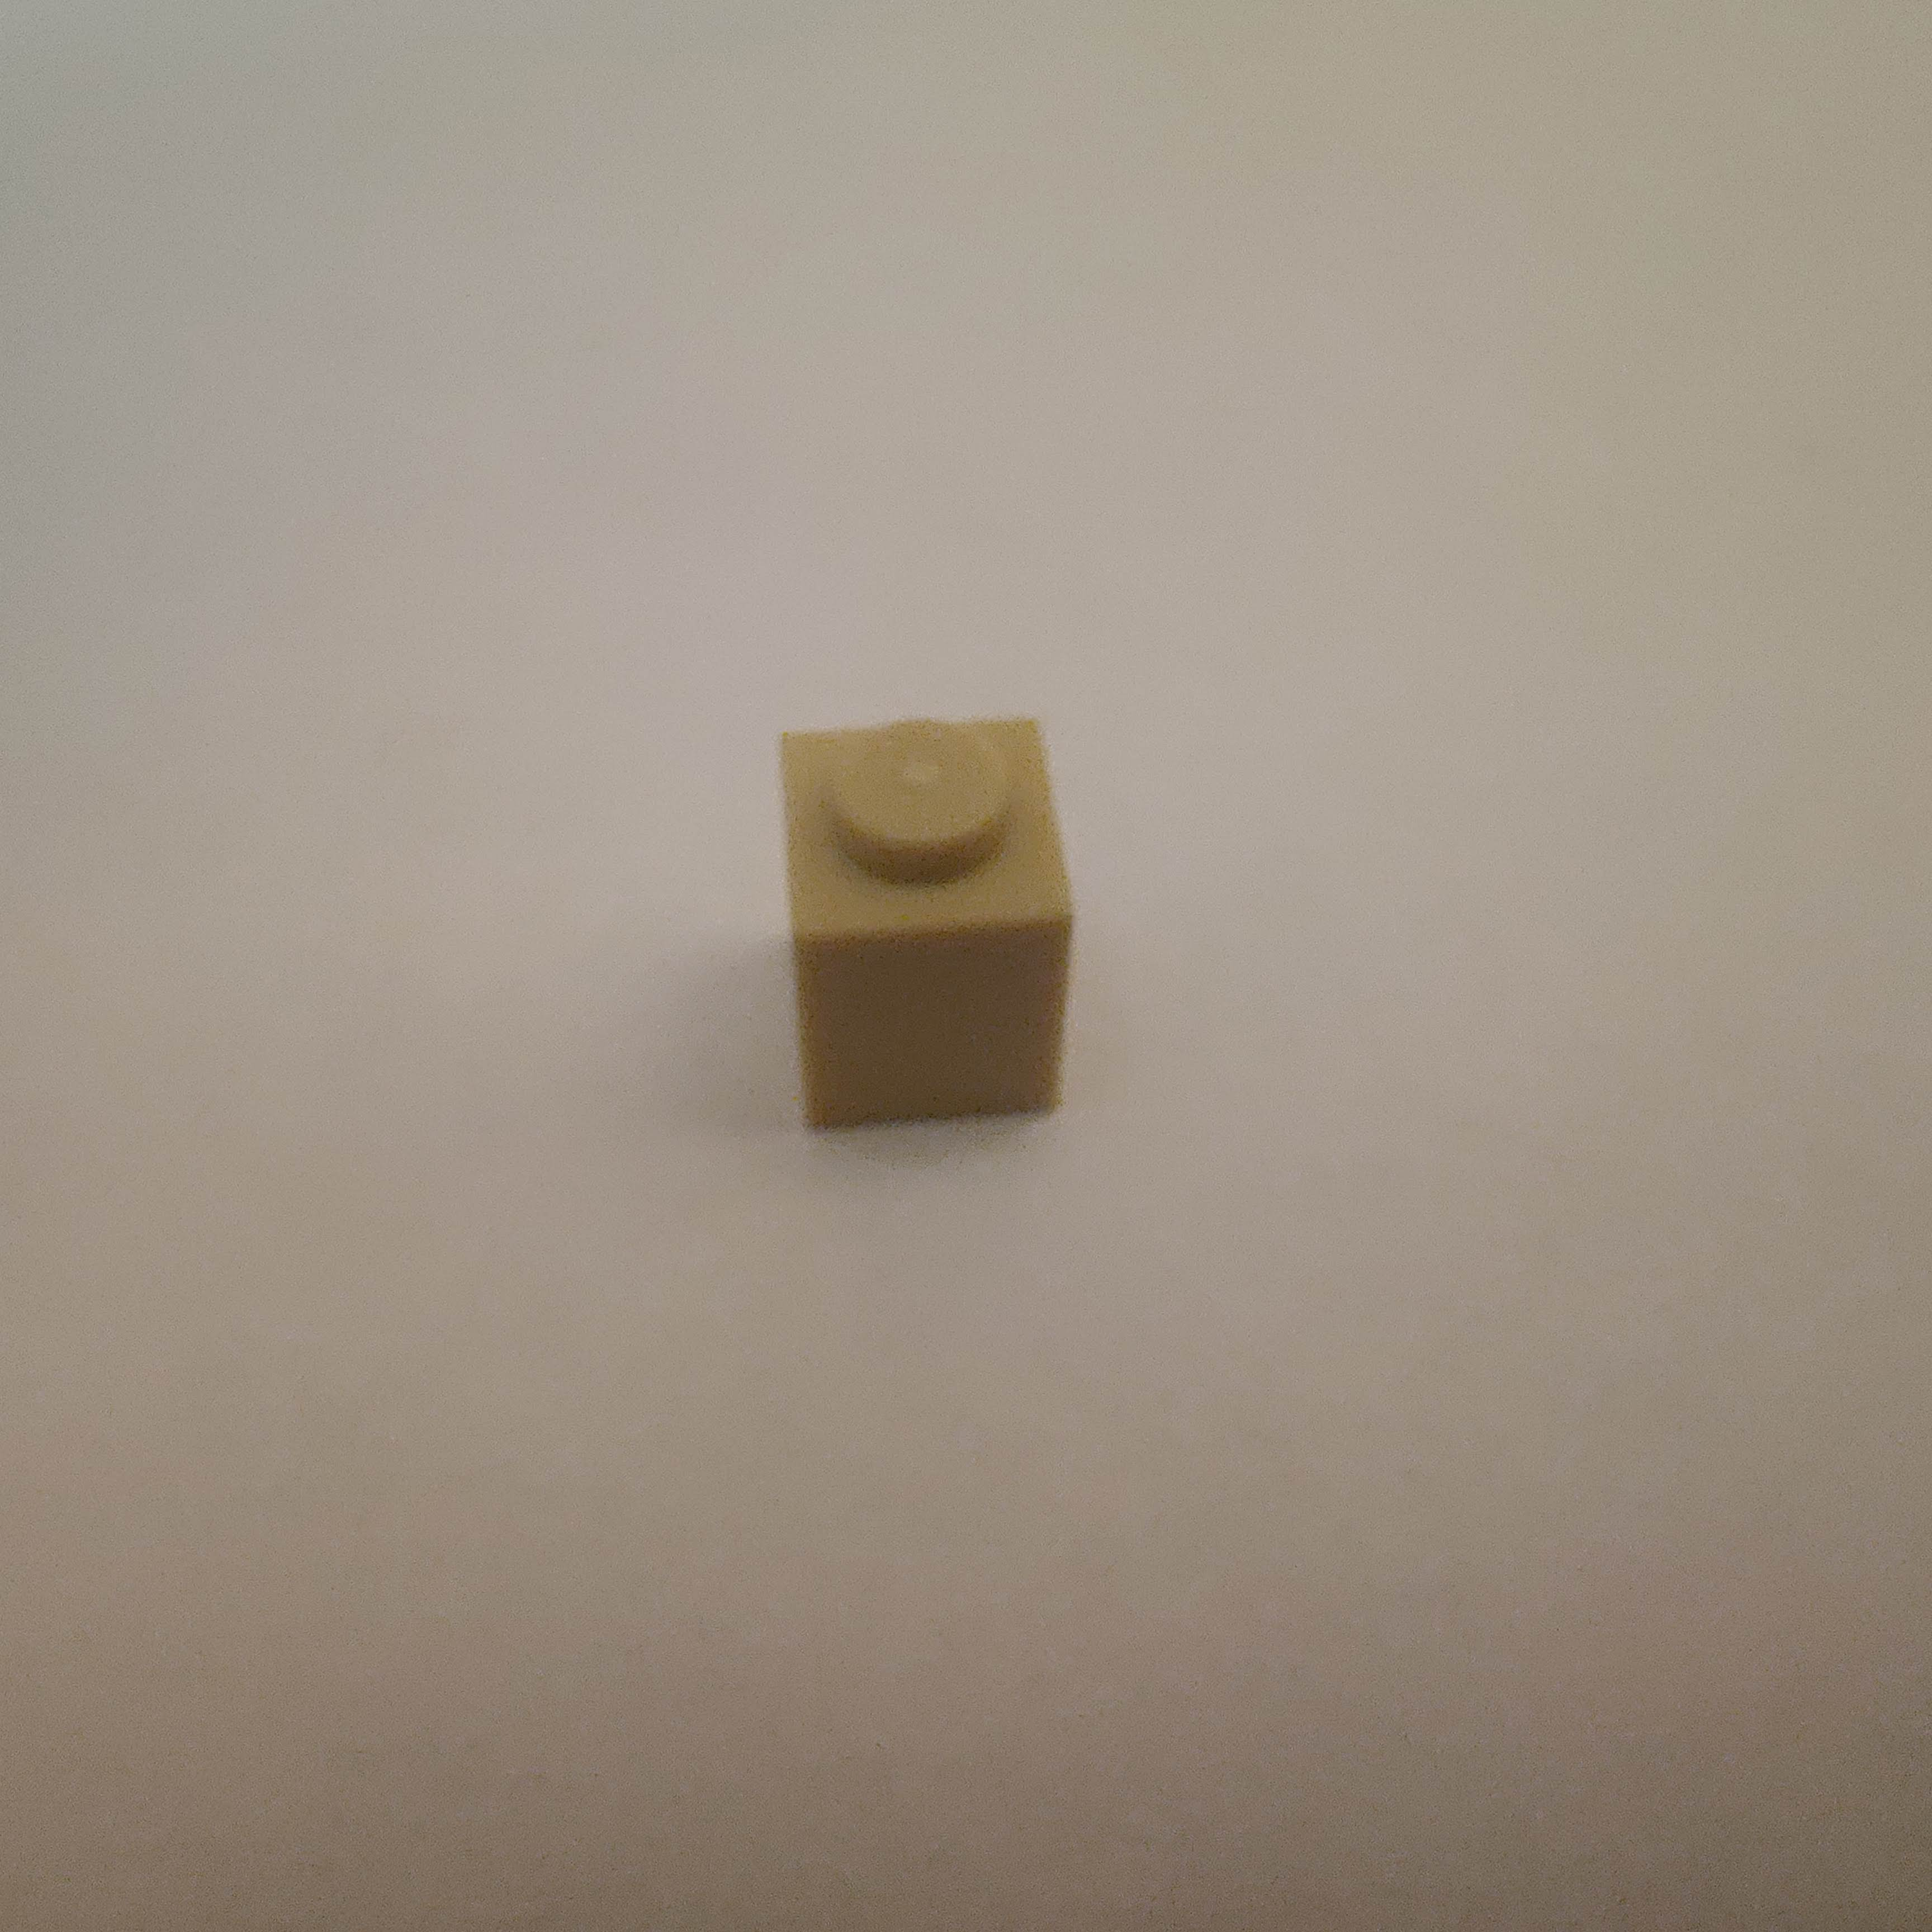
\includegraphics[width=\textwidth]{photographed images/18.jpg}
    \end{subfigure}
    \begin{subfigure}[b]{0.2\textwidth}
        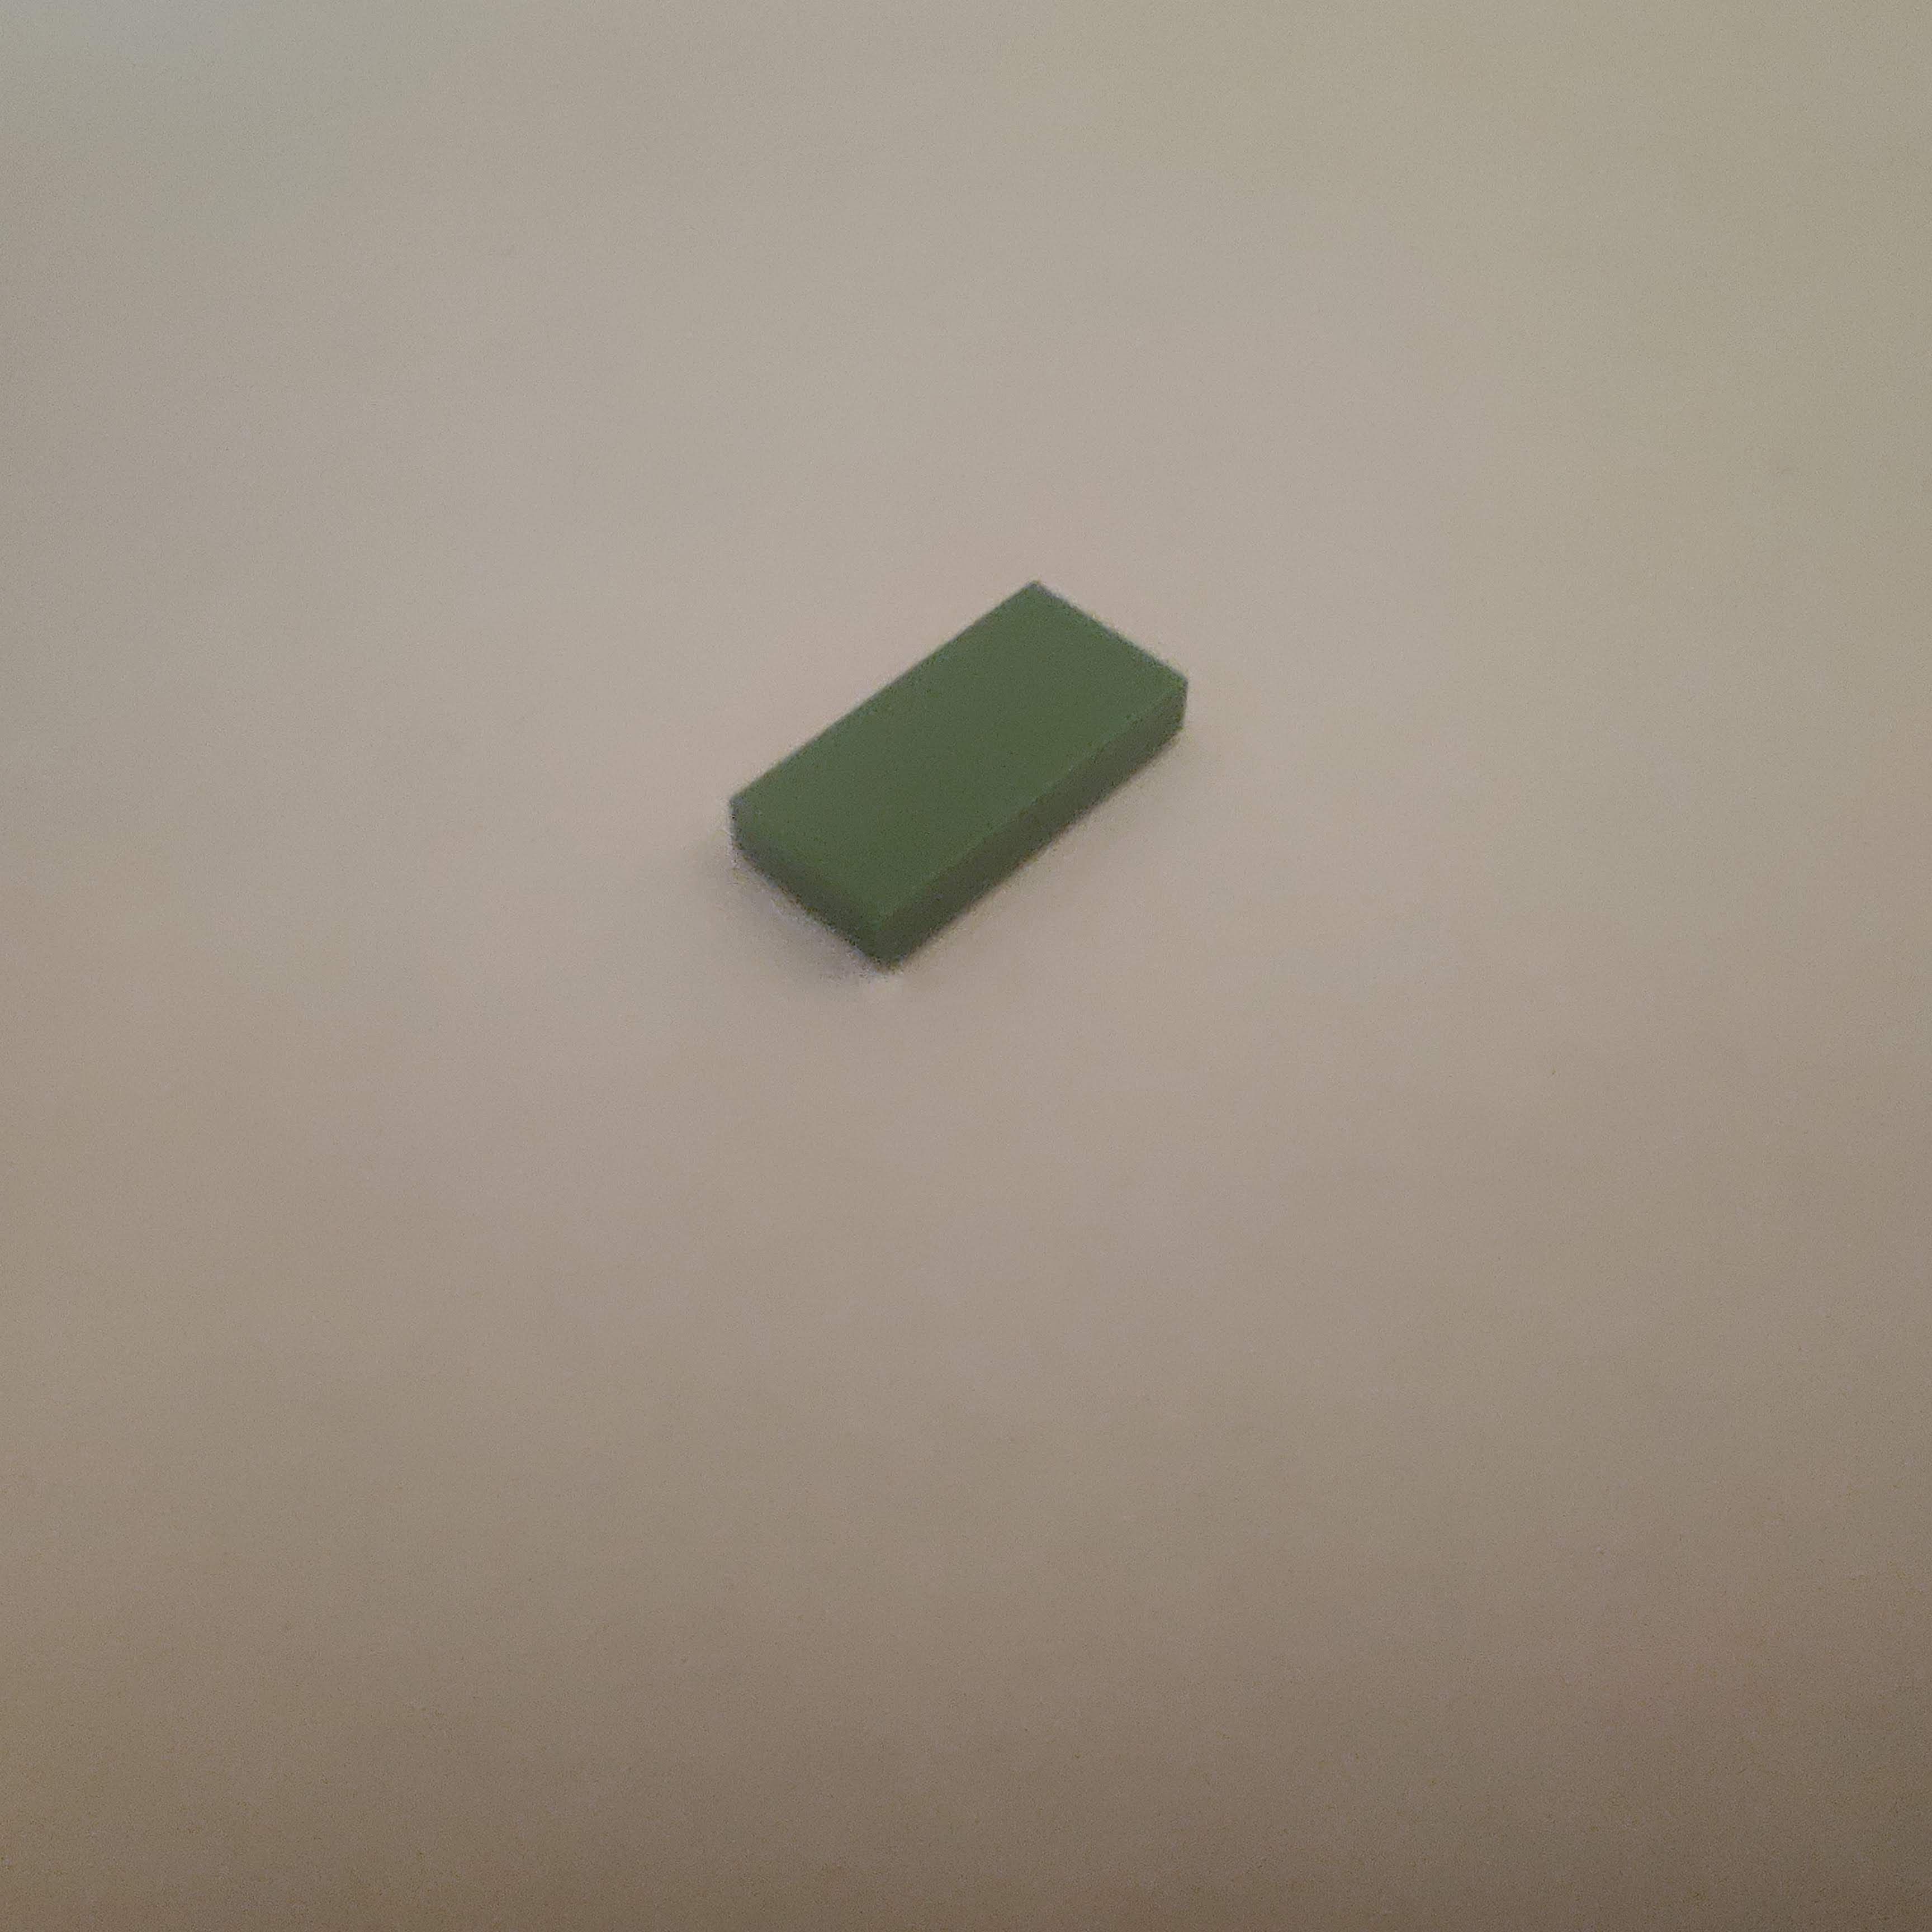
\includegraphics[width=\textwidth]{photographed images/19.jpg}
    \end{subfigure}
    \begin{subfigure}[b]{0.2\textwidth}
        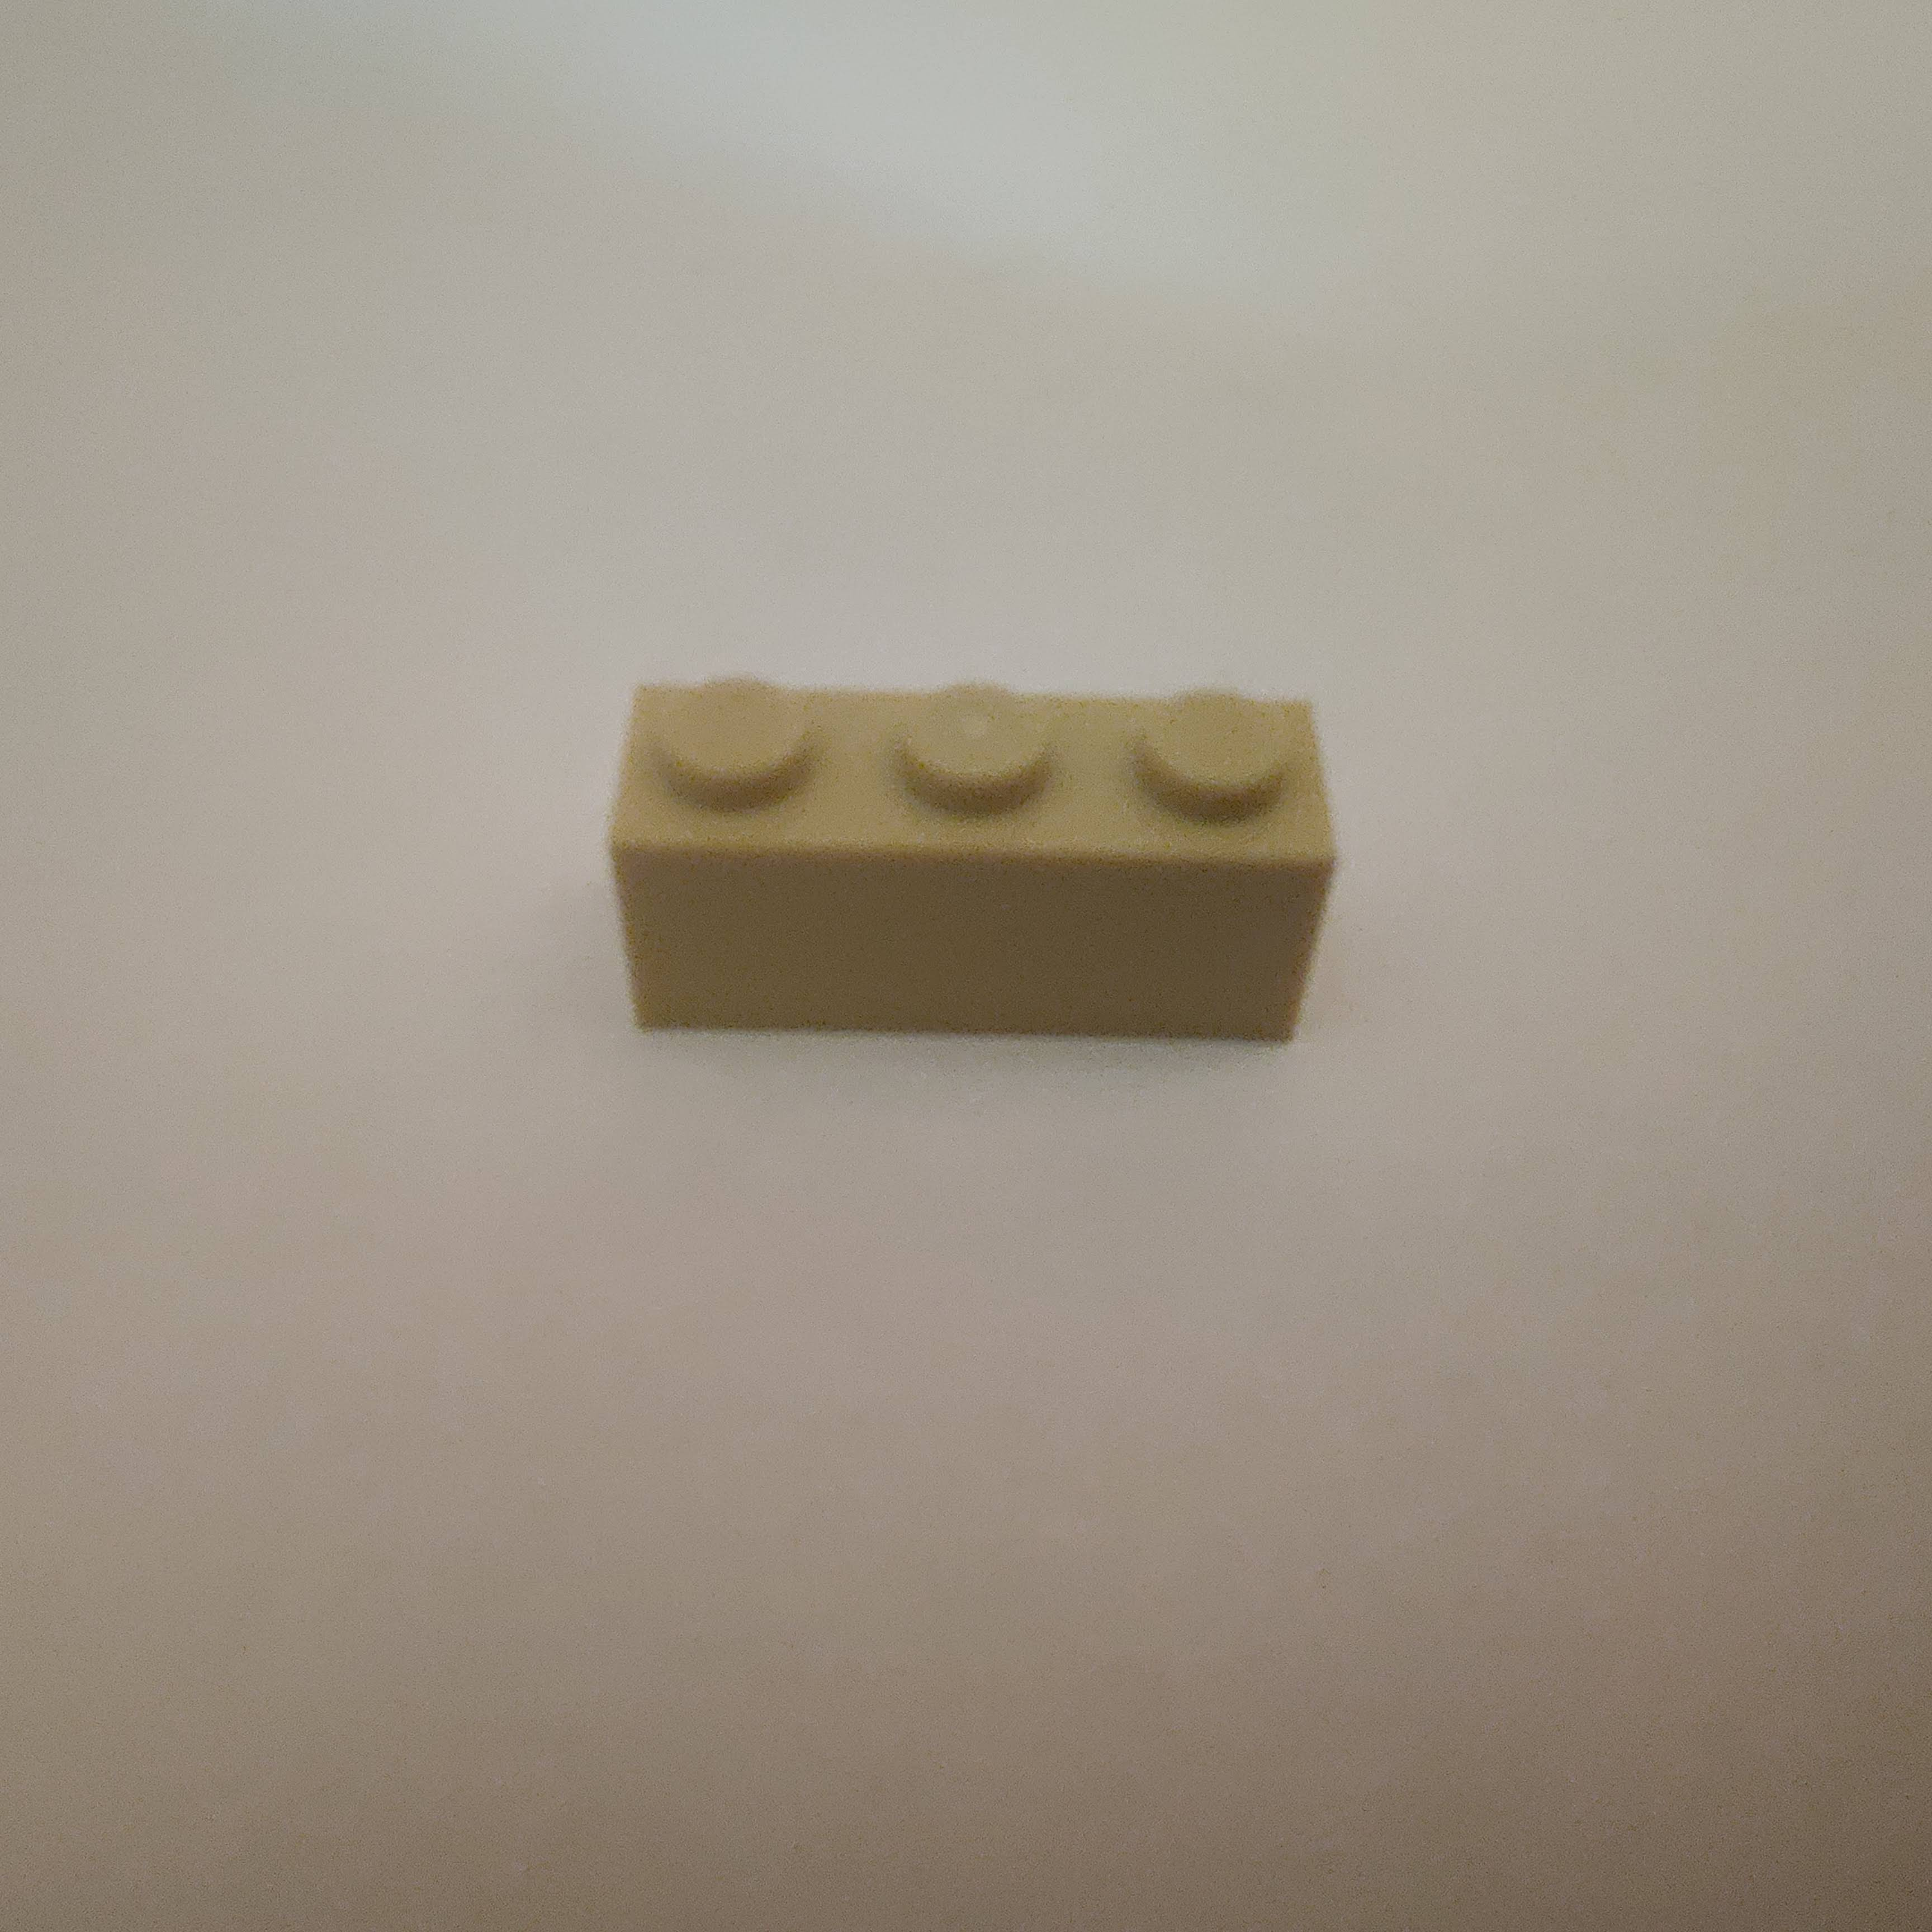
\includegraphics[width=\textwidth]{photographed images/20.jpg}
    \end{subfigure}
    \begin{subfigure}[b]{0.2\textwidth}
        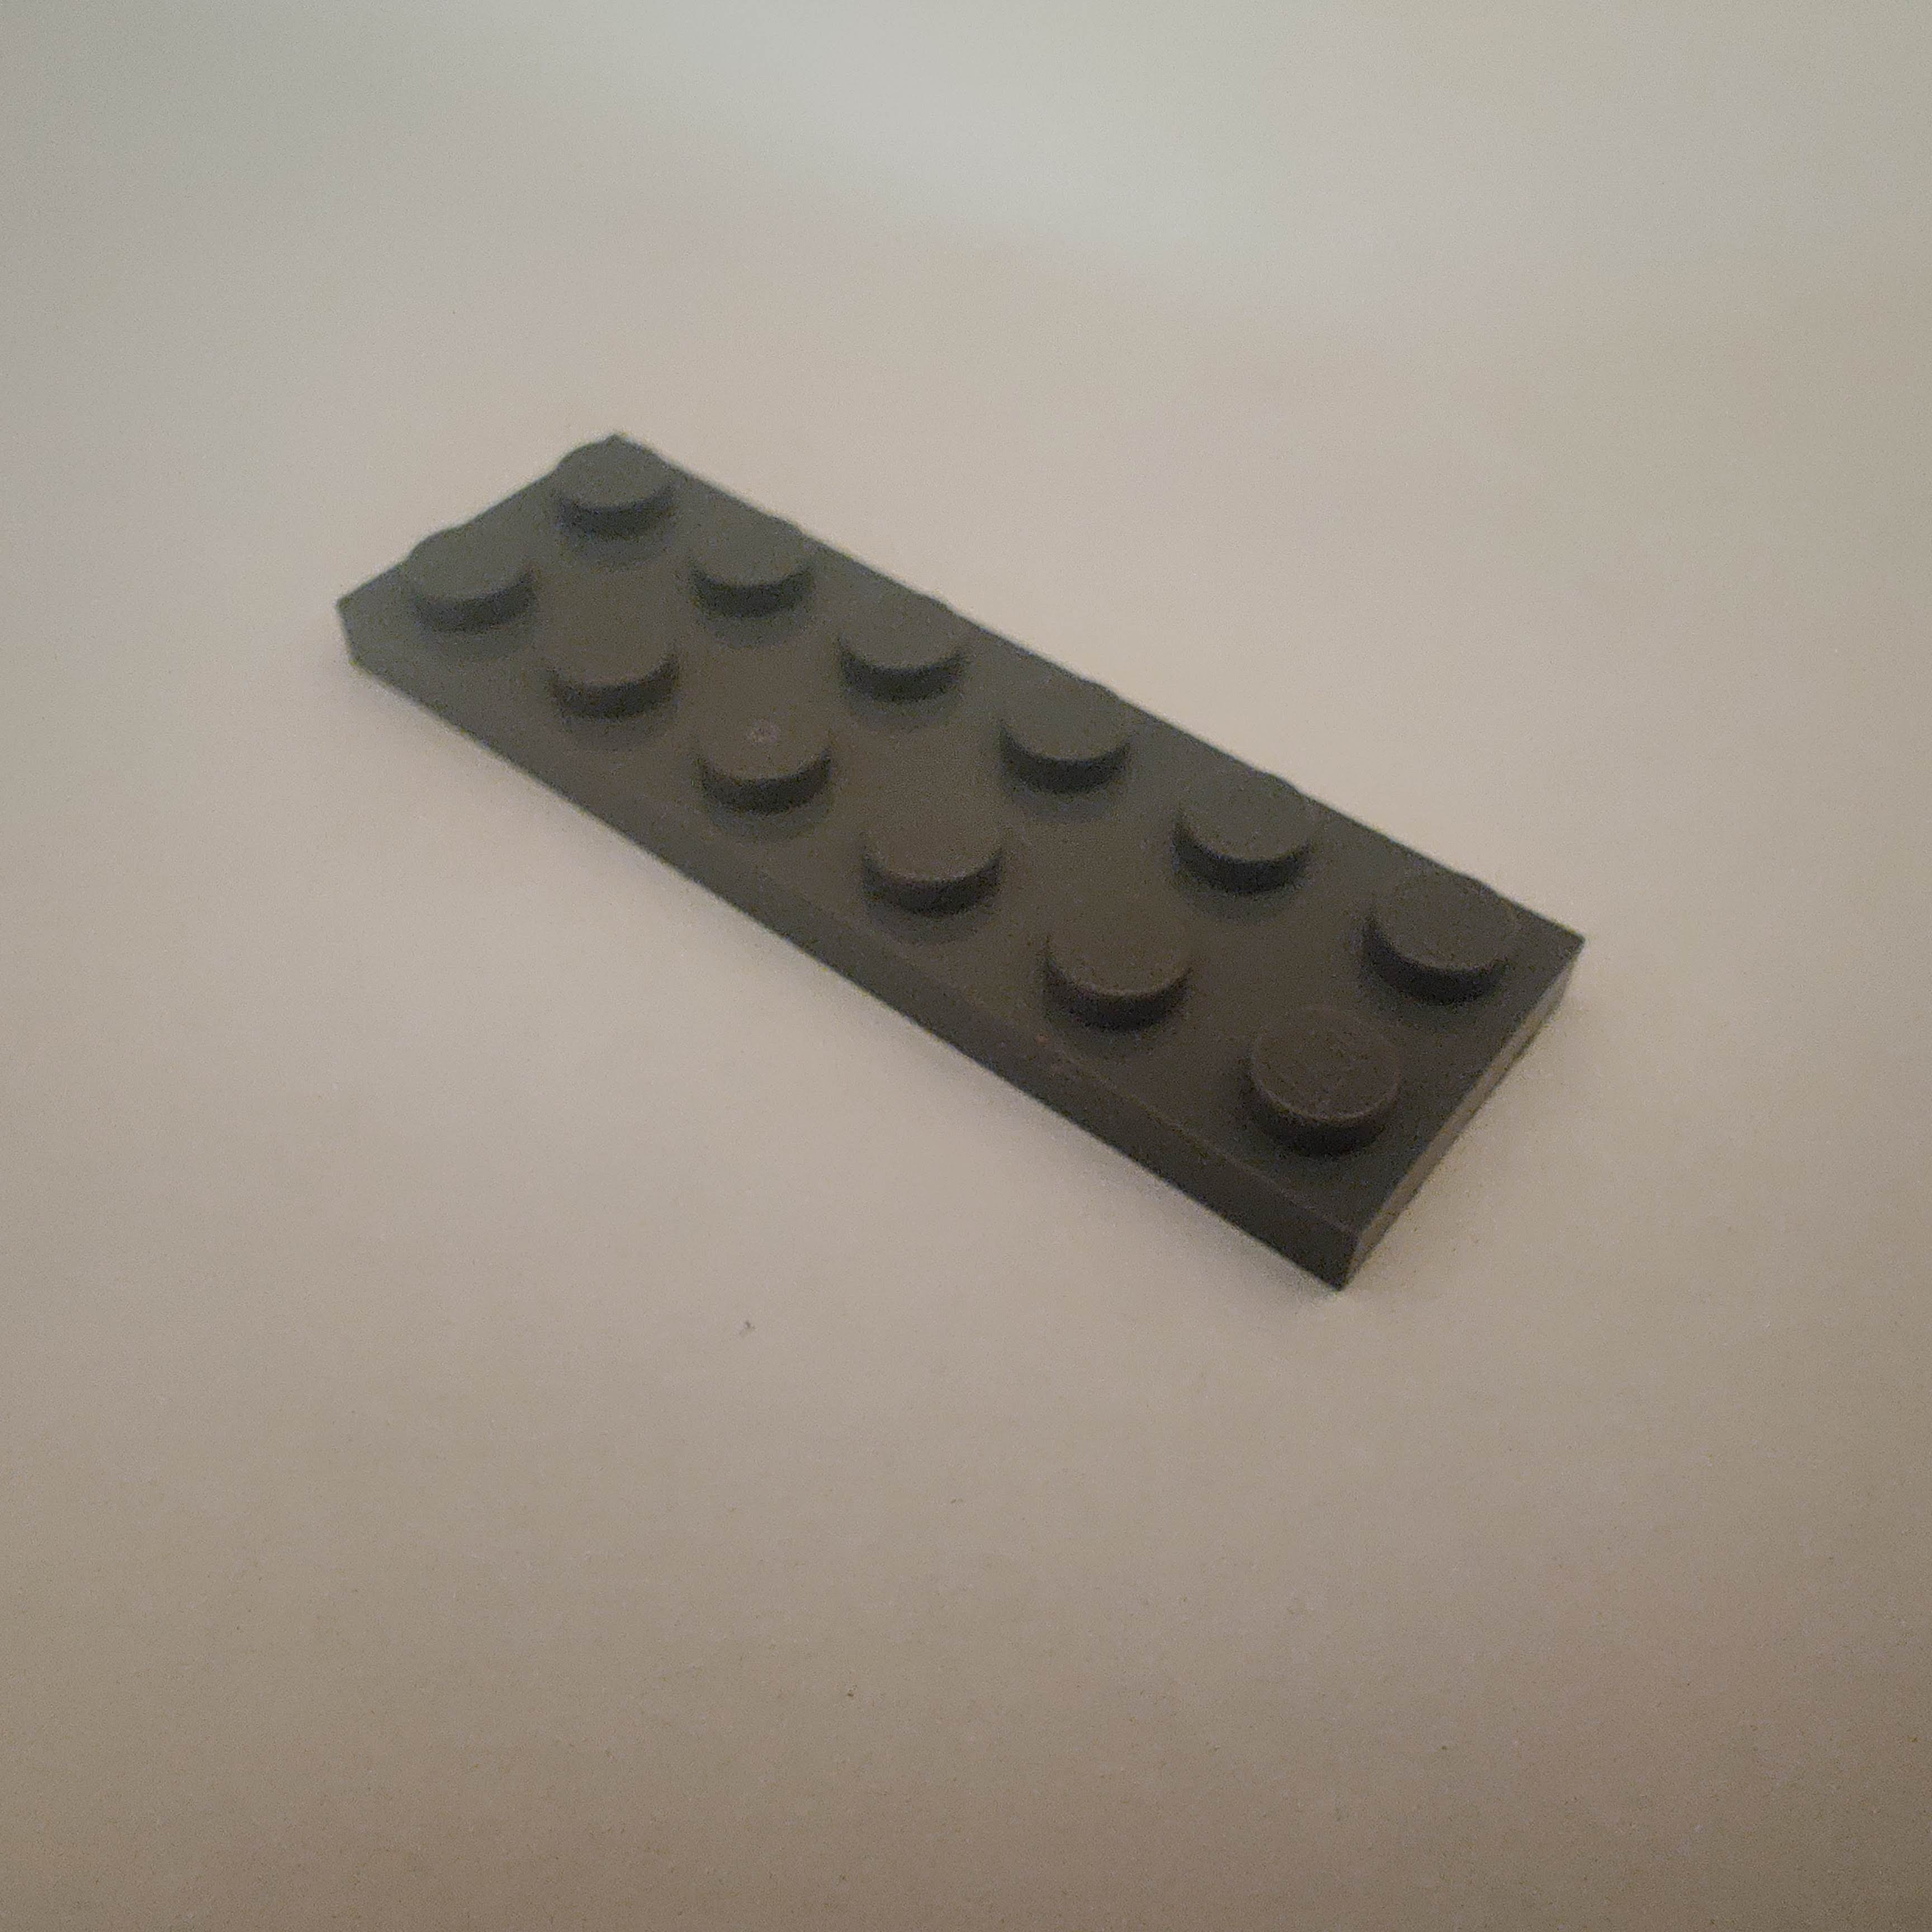
\includegraphics[width=\textwidth]{photographed images/21.jpg}
    \end{subfigure}
    \begin{subfigure}[b]{0.2\textwidth}
        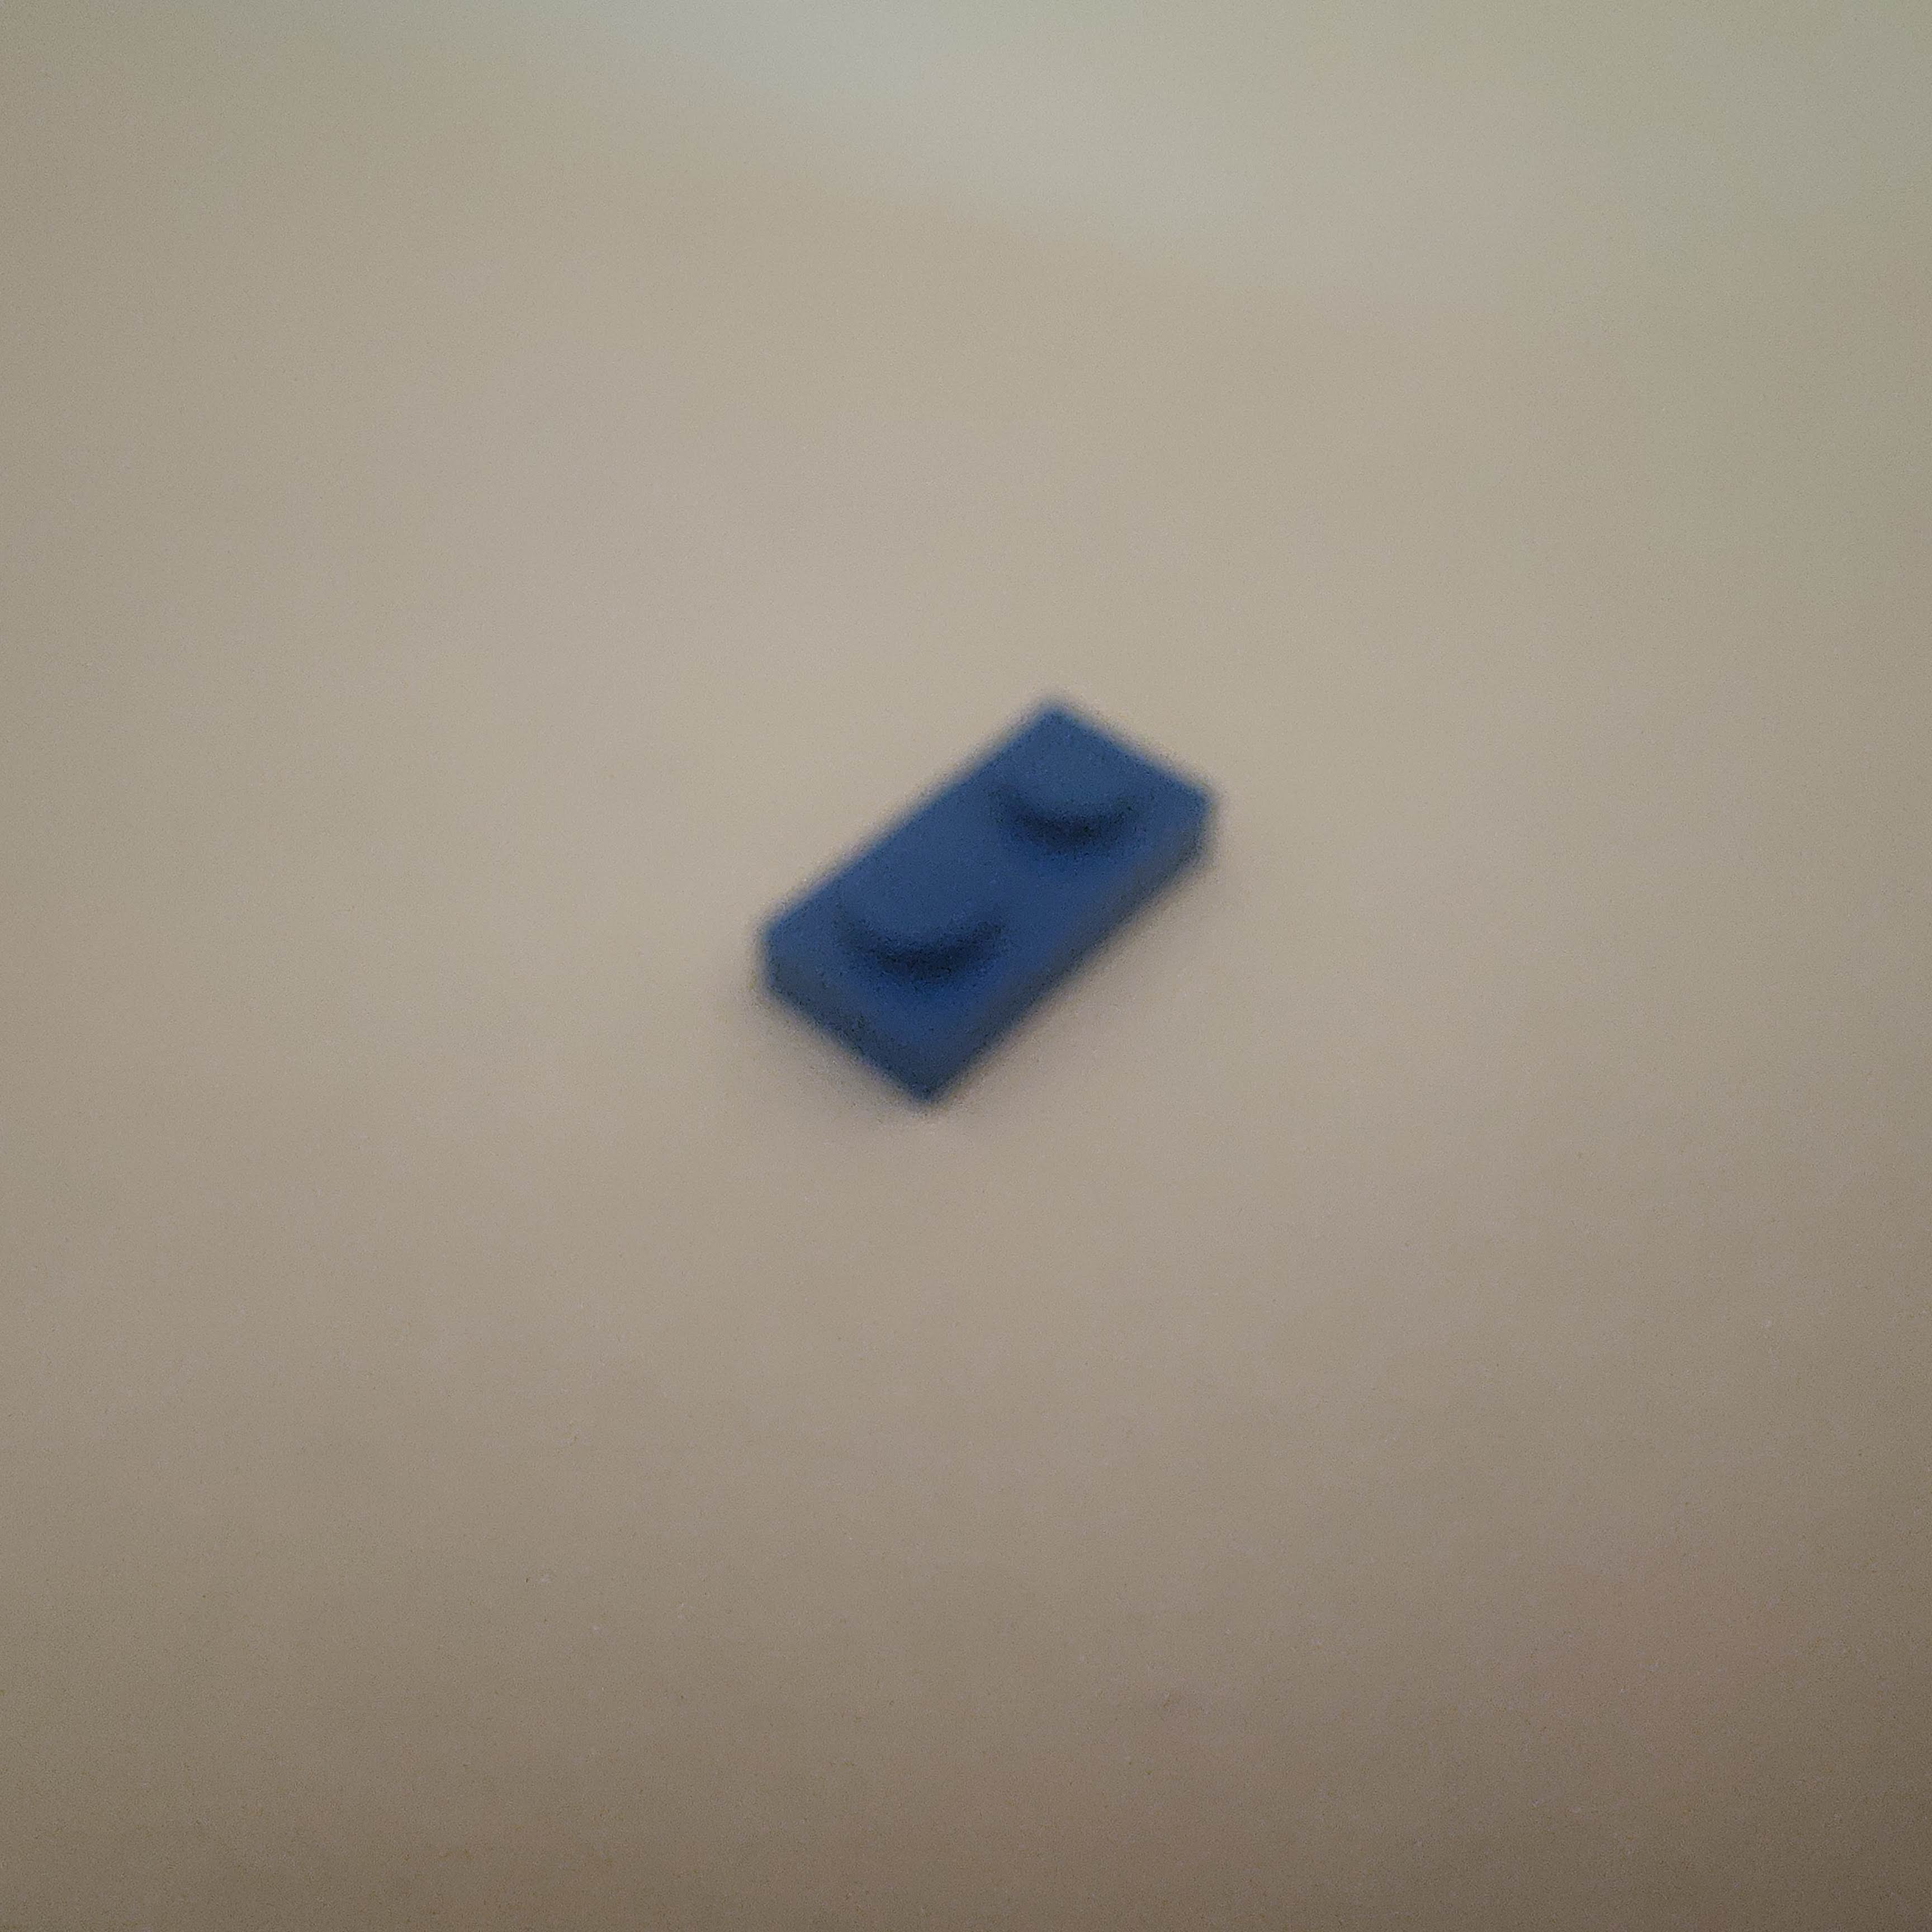
\includegraphics[width=\textwidth]{photographed images/22.jpg}
    \end{subfigure}
    \begin{subfigure}[b]{0.2\textwidth}
        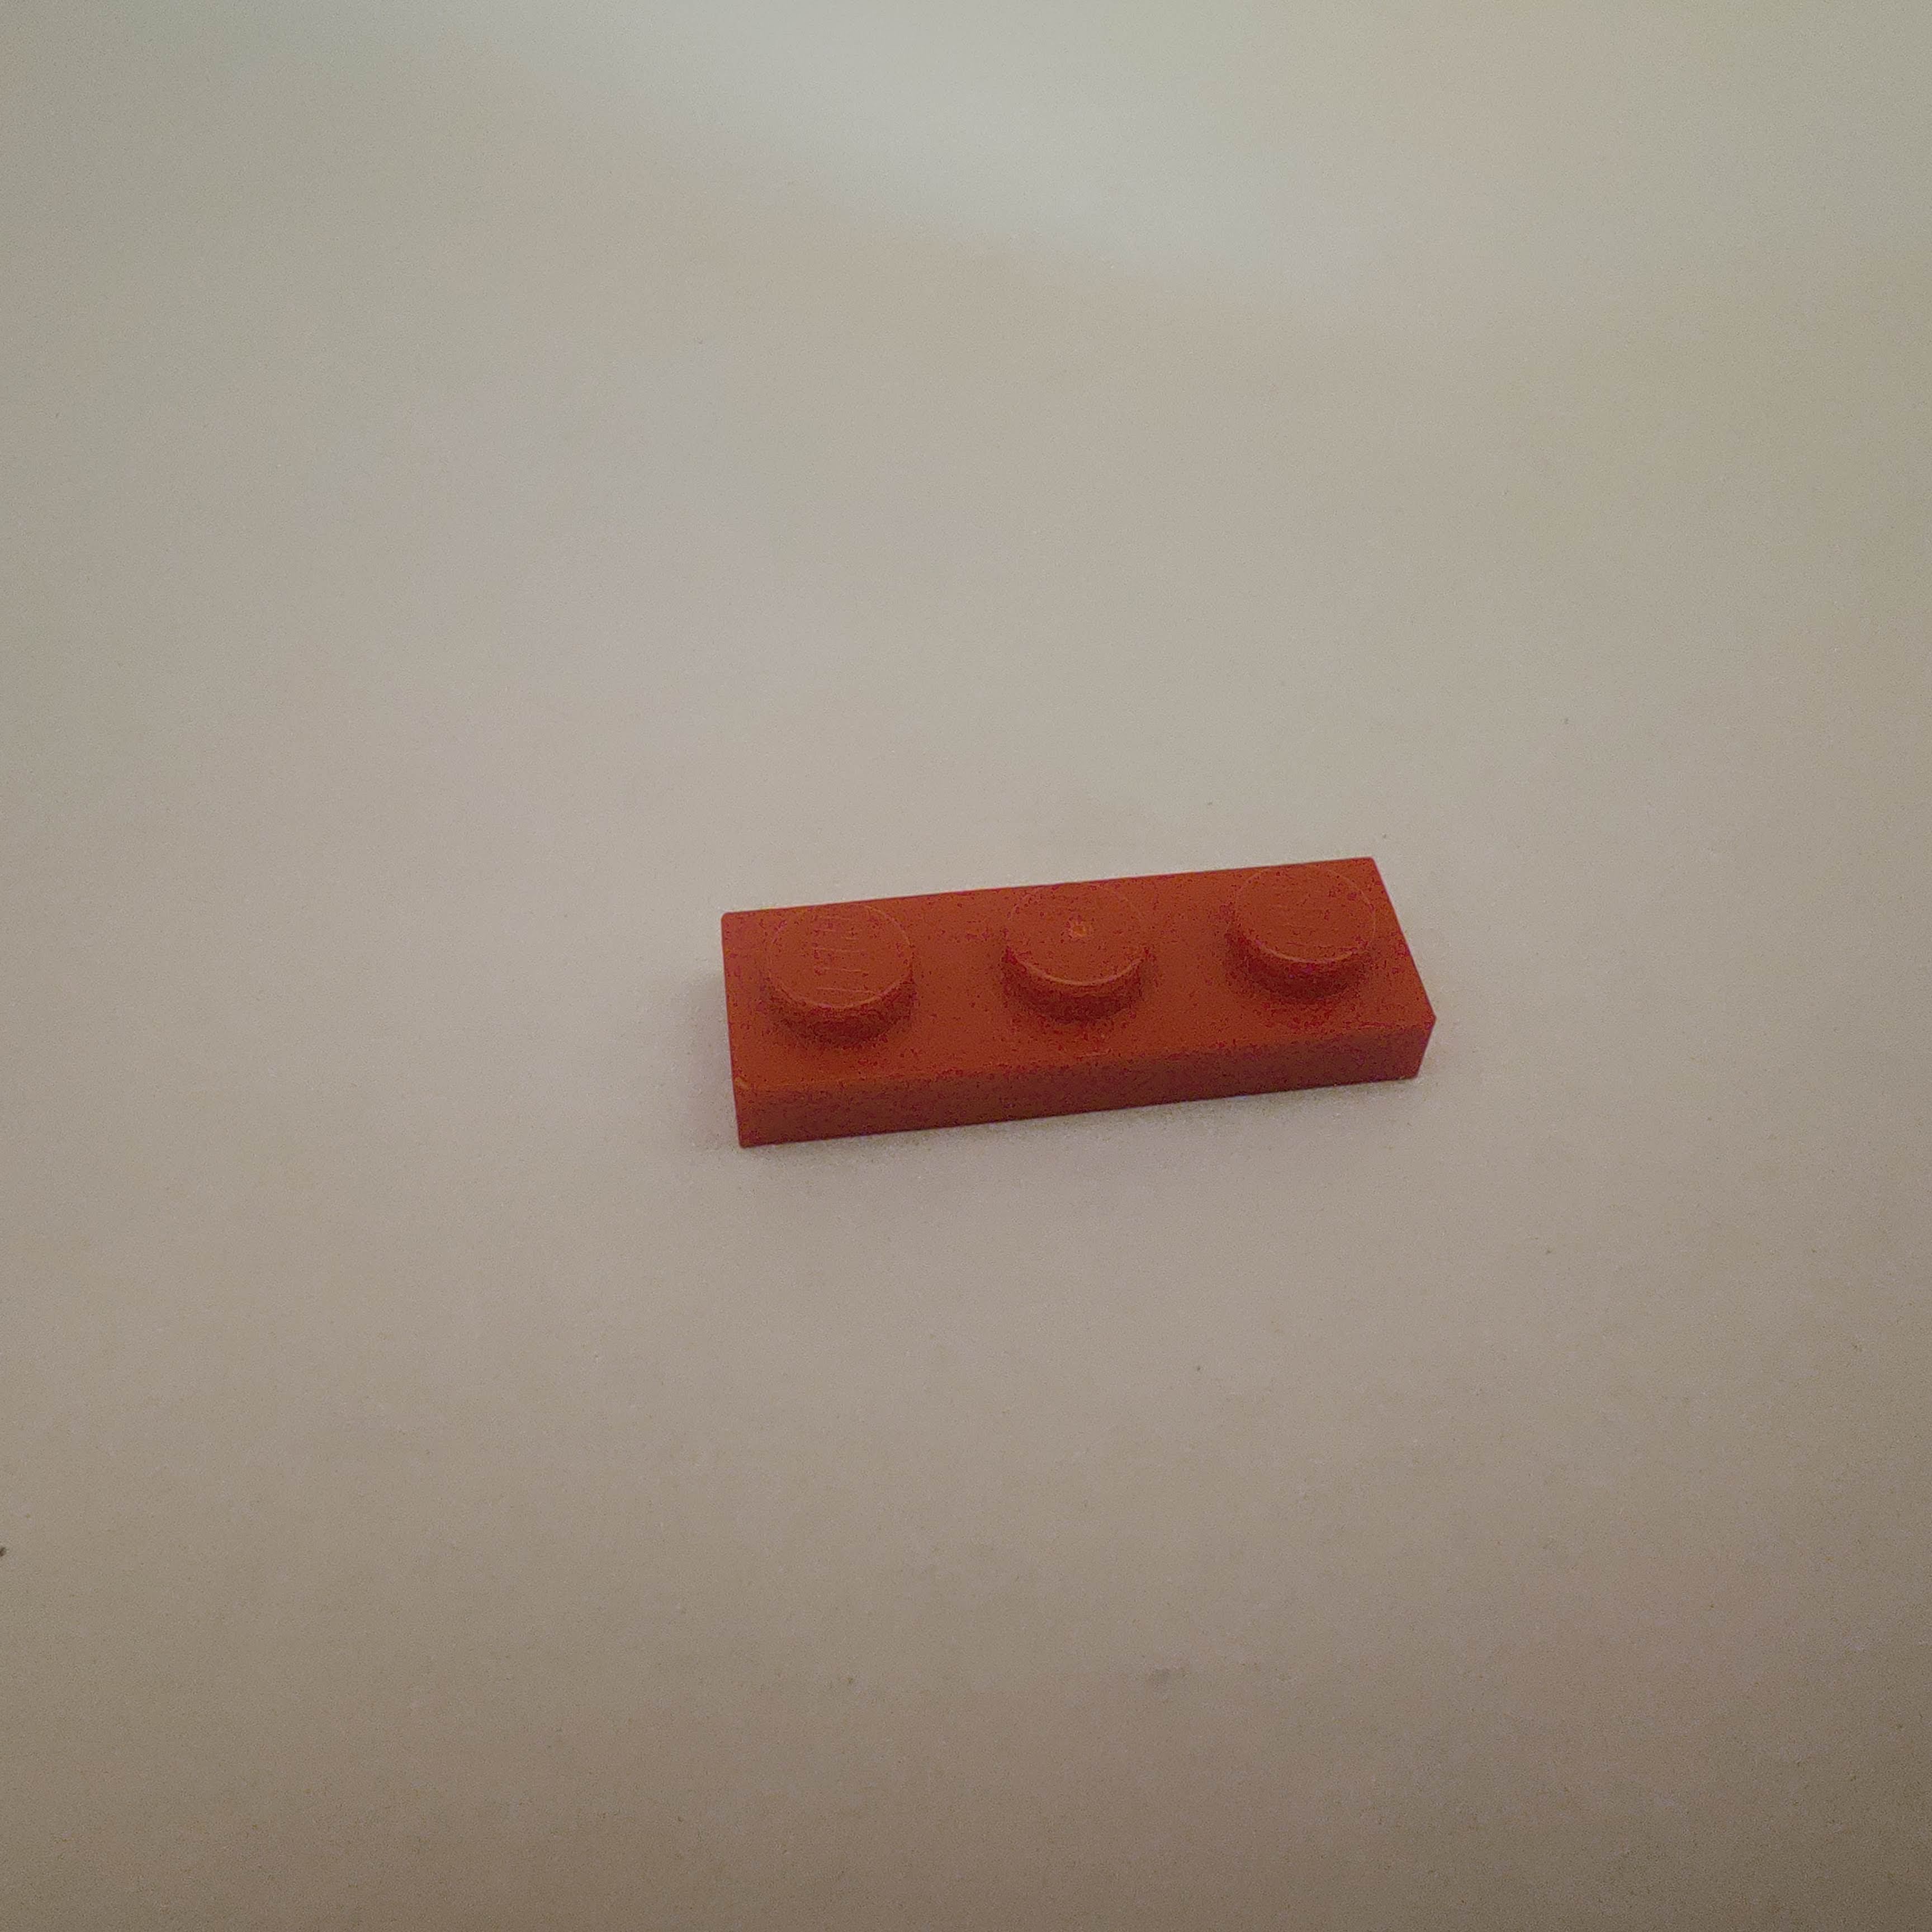
\includegraphics[width=\textwidth]{photographed images/23.jpg}
    \end{subfigure}
    \begin{subfigure}[b]{0.2\textwidth}
        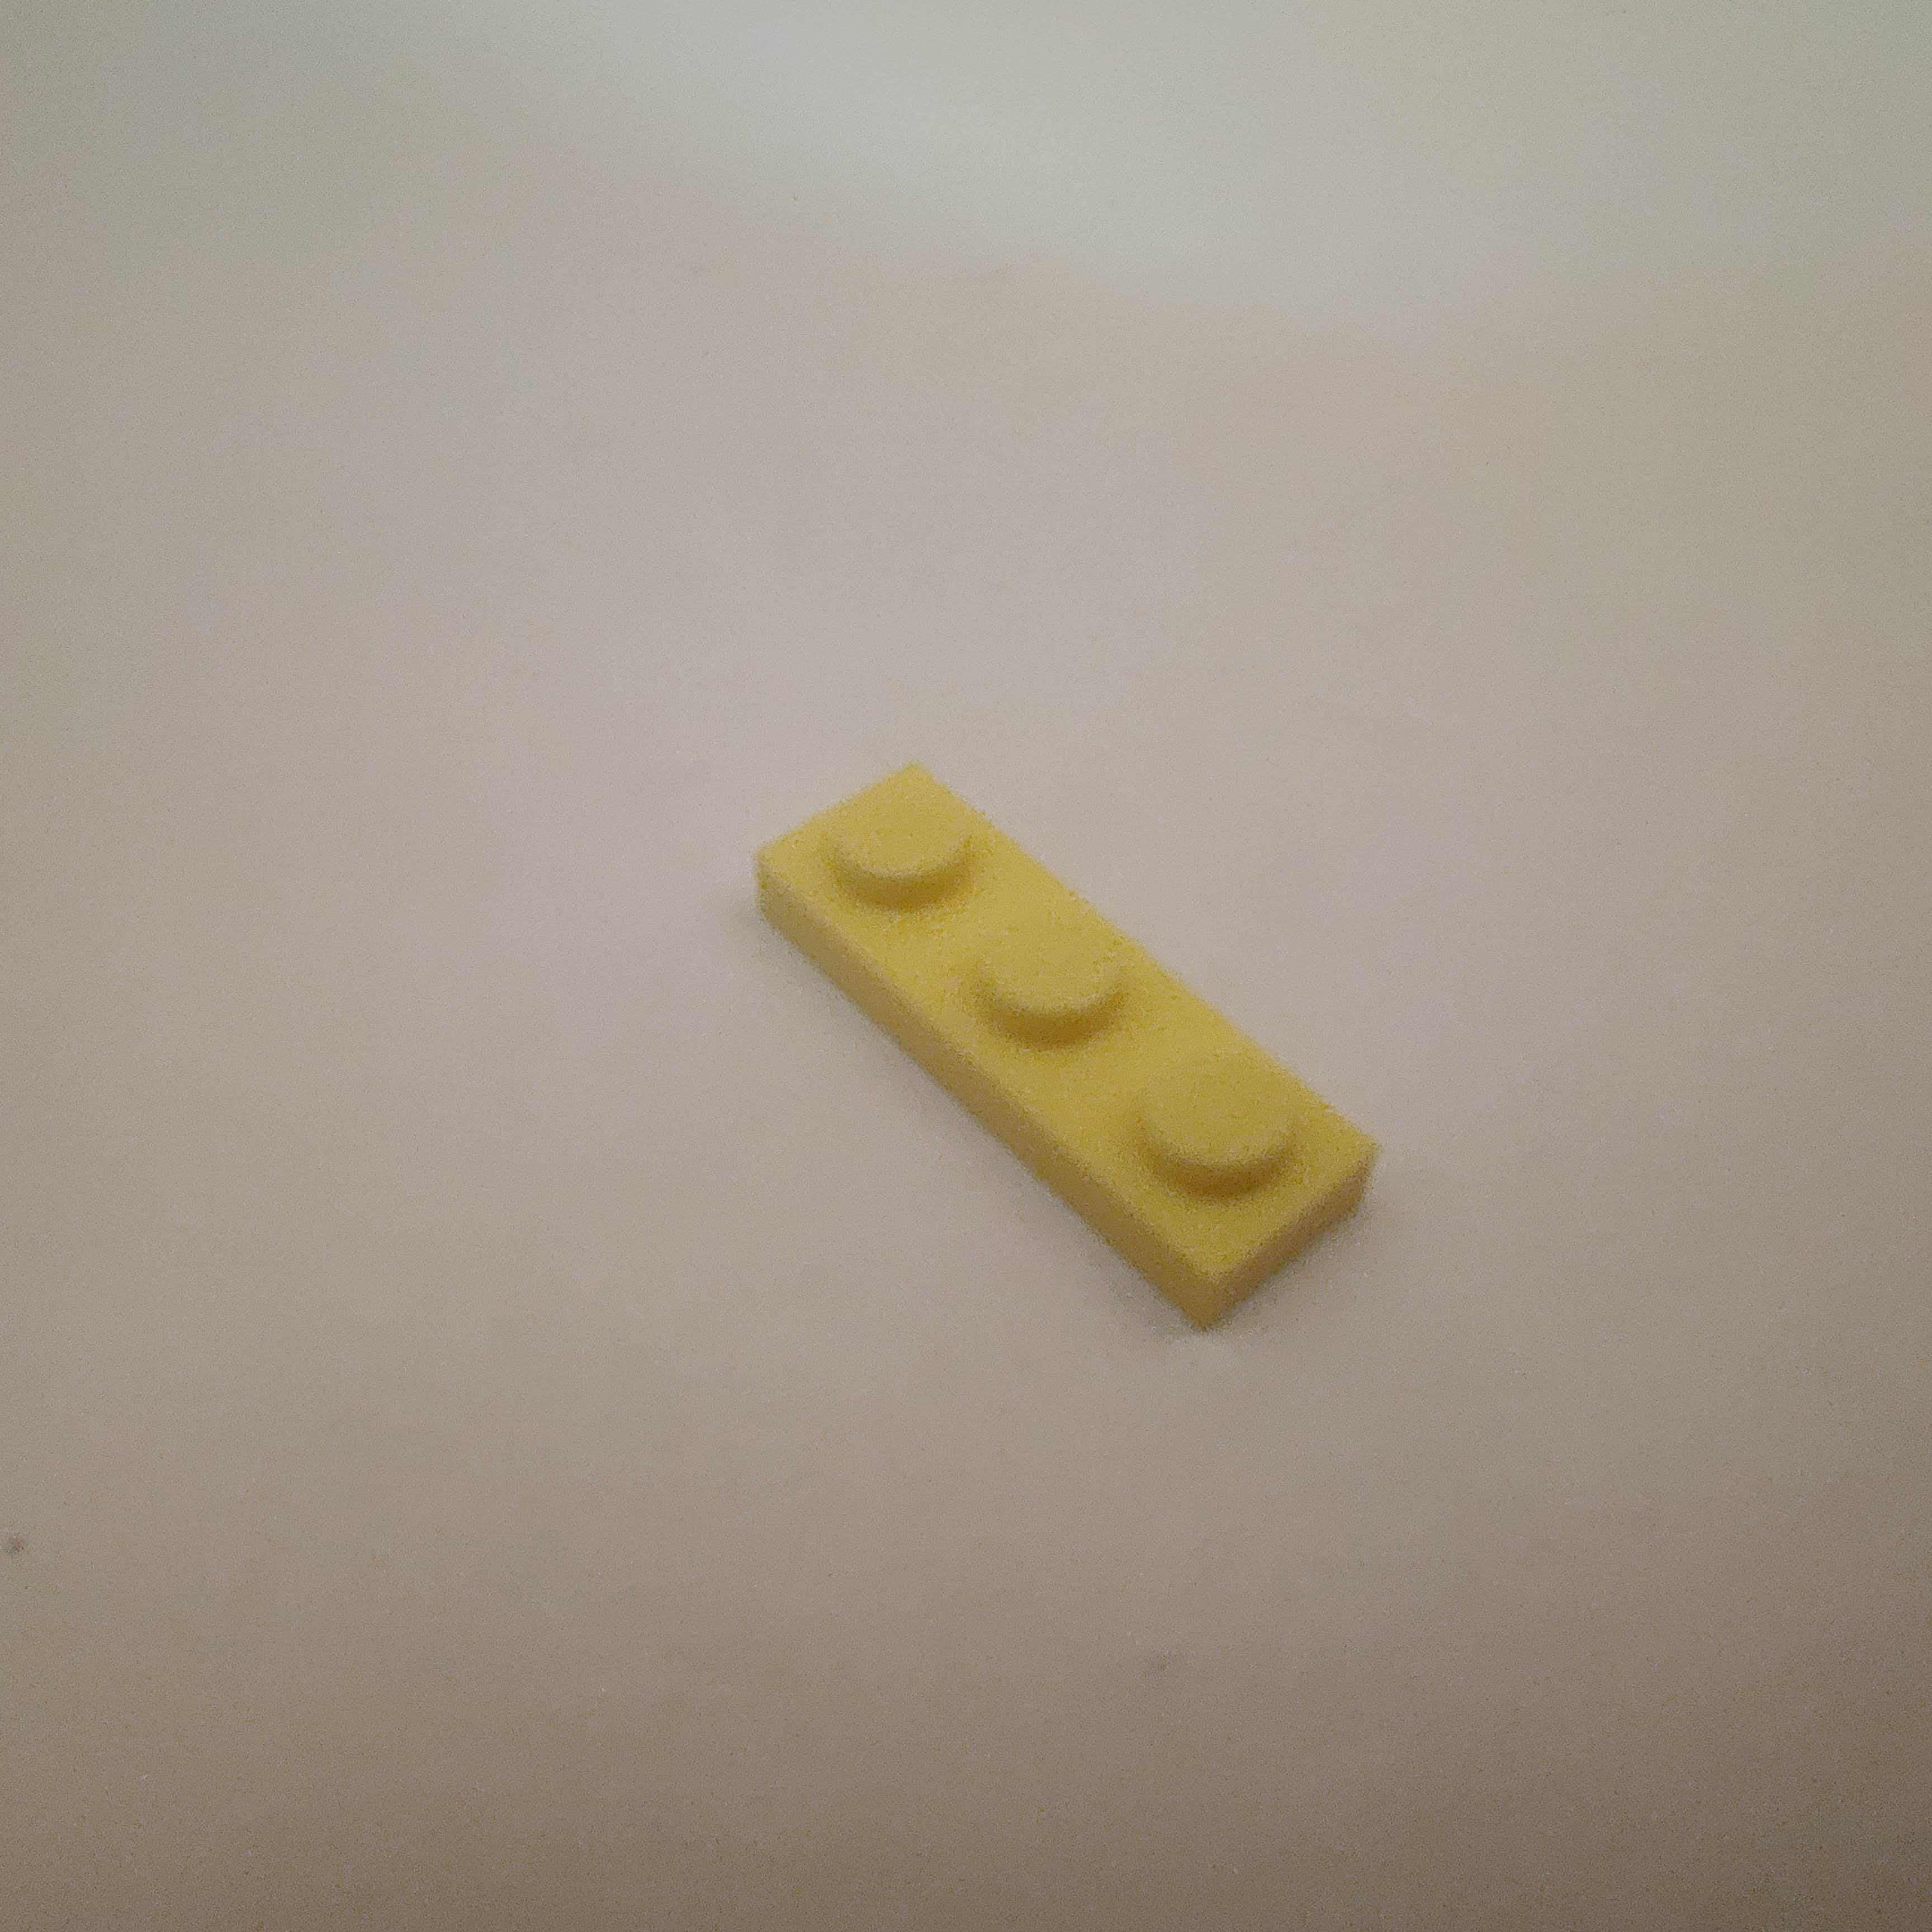
\includegraphics[width=\textwidth]{photographed images/24.jpg}
    \end{subfigure}
    \caption{Example of the photographed dataset}
\end{figure}

\clearpage

\section{VAE}
\subsection*{a.}
\begin{enumerate}
  \item The pipeline fore this project is:
        1024x1024 Images $\rightarrow$ Resize to 64x64 $\rightarrow$ Augment the data by adding mirrored
        images to the dataset $\rightarrow$ Train VAE $\rightarrow$ Plot the images across the latent
        space.
  \item Vanilla VAE
  \item 2D latent space was chosen since it is easy 
        to show the latent space and
        do latent space arithmetic or transformations.
  \item For the real life legos, converting and augmenting data takes 
        about 1 minute and training takes 14 seconds.
        For the rendered legos, 1.5 minutes and 1.7 minutes.
  \item I was unable to do 1024x1024 training since I didn't have enough vram for it,
        but for the repo that I cloned, the highest dimesion that was able to still
        be graphed was 64x64. So we had to lower the resolution and we decided on
        64x64 since it was still relatively fast to train and it was the biggest
        we can do.
  \item The biggest challenge was trying to get the dataset to actually
        work with the VAE that was found. What was really helpful was
        looking at the shapes of the numpy arrays if you get operation errors.
        In addition, I wasn't sure how to get the graphs working with colors
        so I decided to do only greyscale instead.
\end{enumerate}

\subsection*{b. Passing Original Images Through VAE (Real Legos)}
\begin{center}
  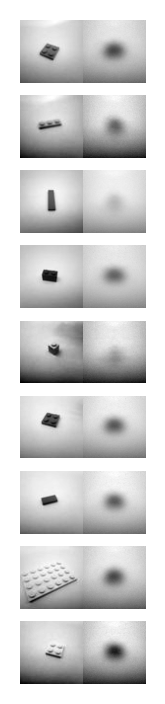
\includegraphics[scale=1]{10_original-lego-dataset}
\end{center}

The VAE managed to capture the color of the pieces,
however the shape of the pieces were lost.
There is one outlier which is the large float white piece;
that piece's color and shape were not captured.

\subsection*{c. Graphs of the Latent Space (Real Legos)}

Here is a plot of the dataset on the latent space:

\begin{center}
  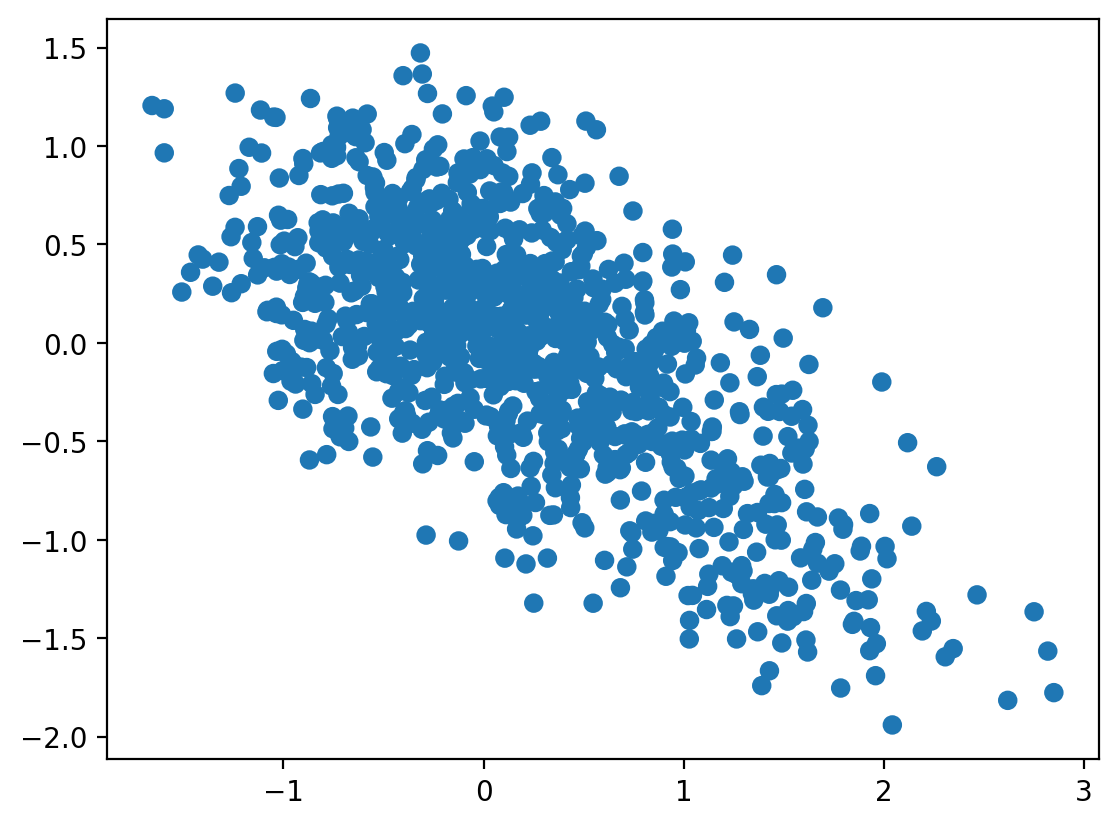
\includegraphics[scale=0.75]{latent_space-lego-dataset}
\end{center}

Here is a plot of images sampled across the latent space:

\begin{center}
  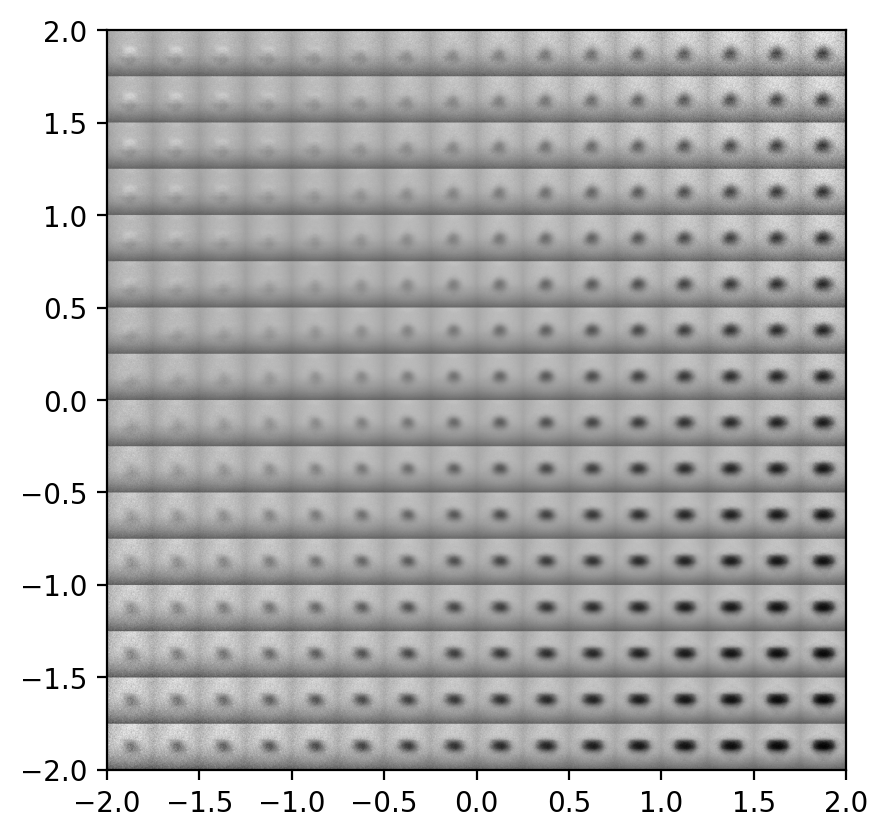
\includegraphics[scale=1]{latent_space_examples-lego-dataset}
\end{center}

The area nearby the origin in latent space is very blurry and hard
to distinguish between the lego and the background. The farther
out you go from the origin, the more the lego looks like but
there is more noise added to the image.

The two features that the VAE were able to pick up on were the color
of the lego and a very general shape or rotation of the piece.

I think the images are very reasonable given the data.

\subsection*{d. Interpolation of Two Places in Latent Space (Real Legos)}
\begin{center}
  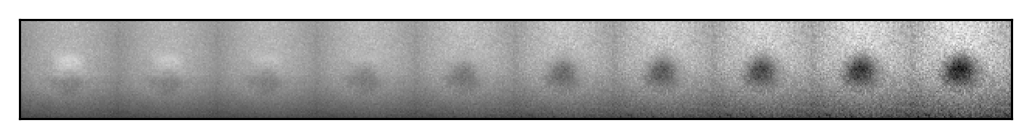
\includegraphics[scale=0.9]{interpolation-lego-dataset}
\end{center}

I took two points in the latent space (-2, 2) to (2, 2) and interpolated
the space between these points with the VAE.


\subsection*{b. Passing Original Images Through VAE (Rendered Legos)}
\begin{center}
  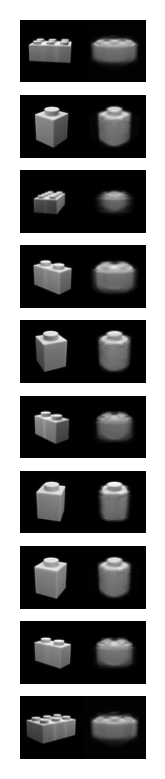
\includegraphics[scale=1]{10_original-lego-blender-4}
\end{center}

Compared to the real legos, the VAE managed to better capture
the overall shape of the legos. 
This is probably due to the more consistent framing of the legos
in the center of the image.
However, some of the legos when
look blurry as if it VAE were rotating the lego.

\subsection*{c. Graphs of the Latent Space (Rendered Legos)}

Here is a plot of the dataset on the latent space:

\begin{center}
  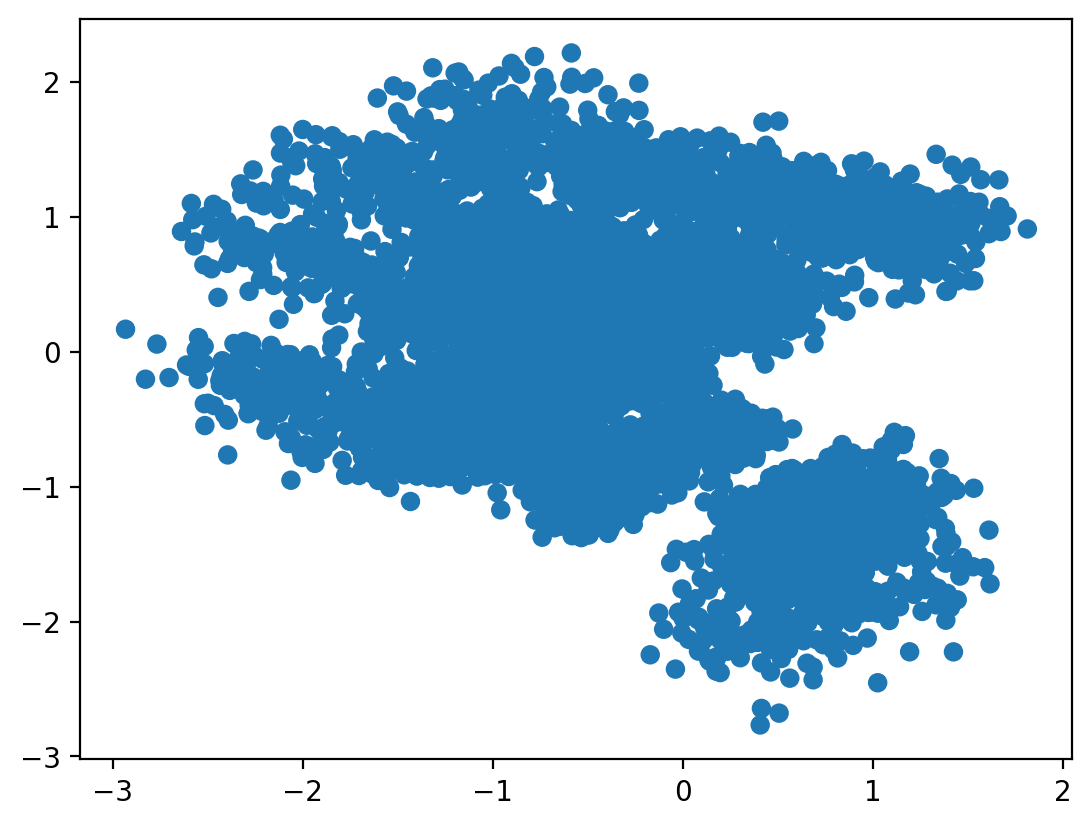
\includegraphics[scale=0.75]{latent_space-lego-blender-4}
\end{center}

Here is a plot of images sampled across the latent space:

\begin{center}
  \includegraphics[scale=1]{latent_space_examples-lego-blender-4}
\end{center}

Compared to the latent space of the real legos, there are clear
areas where different types of bricks are located in the latent space.
Like the other VAEs that were demonstrated in the classroom,
thee are regions in the space where the VAE is blending between two or
more different types of bricks.

The features that the VAE were able to pick up on were
the type of bricks (1x1, 2x2, 2x4, 2x4). Since there
wasn't very much in difference in the colors of the bricks,
they are all the same greyish color.

I think the images are very reasonable given the data.

\subsection*{d. Interpolation of Two Places in Latent Space (Rendered Legos)}
\begin{center}
  \includegraphics[scale=0.9]{interpolation-lego-blender-4}
\end{center}

I took two points in the latent space (-1, -1) to (1, 1) and interpolated
the space between these points with the VAE.
\newpage
\section{Project Proposal}
\begin{enumerate}[(a)]
    \item What are the effects that you hope to create in your project? How do you think the effects will support the narrative of the video? (that is, why are the effects you propose suitable to the context?)
    \begin{itemize}
        \item Our problems are object style transfer with captioning. Style transfer takes a content and a style, then transform the content due to that style. A "style" in this context refers to both the geometry of the input object and its textural data. Captioning takes a scene and generates a short text description based on all the content within the scene. Our project idea is to use a scene, which contains multiple 3D objects, and perform style transfer, texturing and captioning.
    \end{itemize}
    \item A storyboard that walks us through what we will see as the video progresses.
    \begin{itemize}
        \item Begin with an overview of the original scene, containing various objects inside of a room, such as desks, chairs, a bed, bookshelves, books, plushie, snacks, etc.
        \item Focus to specific parts and for each object within the scene:
        \begin{enumerate}
            \item Perform geometric style transfer.
            \item Apply textural style transfer.
        \end{enumerate}
        \item Repeat for multiple style inputs. The first cycle will showcase the fact that the program will apply the style transfer individually to each object, while latter cycles can simply show a before and after transformation process in quick succession.
        \item Caption the scene continuously as objects get transformed.
    \end{itemize}
    \item How are the effects related to one or more of the concepts in the book/course? What other related work is there from the technical or artistic literature that is related to your idea? (research papers, examples of similar effects in videos you’ve seen).
    \begin{itemize}
        \item The main concept for this is to experiment with the creative elements of augmentation. As we've seen in class, there are various ways for artists take an original concept, image, or model, and transform it to its own style. \newline \newline
        For instance, in class we referenced Hertzmann's Painterly Rendering, where images are taken and algorithms are used to transform that original image into a painting of that image. Therefore, we plan to do the same with 3D models, taking an original model and transform the style of that model to match whichever style we want it to look like. "Style" would constitute as the general shape of an object and micro-patterns found on the surface of the model.
        \item For style transferring on the 3D models, we will primarily use the 3DSNet research paper. For transferring of textures, we will use StyleRF. For generating captions, we will use ObjectNet3D as part of the pipeline to recognize objects within the scene. 
    \end{itemize} 
    \item Where will you collect your raw image/video/audio data from?
    \begin{itemize}
        \item We will generate our own models by creating scenes in blender. We will then convert the mesh into a point cloud format so that we can have it as an input to the ML models.
    \end{itemize}
    \item What software do you anticipate using to accomplish your goals? What type of coding will need to be done to accomplish the effect?
    \begin{itemize}
        \item We will be studying 3DSNet for style transfer and ObjectNet3D for object classification and using provided code in combination with custom code to produce the models. We will train these models on the ModelNet dataset and our custom datasets.
    \end{itemize} \newpage
    \item What is your strategy/plan of action for realizing your conceptual idea? That is, what tasks need to be performed? What is the rough schedule for these tasks?
    \begin{itemize}
        \item Reproduce the 3DSNet paper.
        \item Fine tune on our custom dataset and perform testing.
        \item Write model for converting scene into point cloud, performing clustering and object identification.
        \item Perform style transfer on each object within the scene.
        \item Use StyleRF to add texturing to objects. 
        \item Generate captions on completed scenes with ObjectNet3D and other relevant tools.
    \end{itemize}
\end{enumerate}

\end{document}  